
% Load basic XeLaTeX style
\documentclass[a4paper,10pt]{article}
\usepackage[top=1.1in, bottom=1.5in, left=1in, right=1in]{geometry}
\usepackage{fontspec}
\usepackage{xunicode}

% Use english
\usepackage{polyglossia}
\setdefaultlanguage{english}

% Load math symbols
\usepackage{amsfonts}
\usepackage{amsmath}
\usepackage{amssymb}

% Define theme colors
\usepackage{xcolor}
\definecolor{mylinkcolor}{RGB}{64,64,128}
\definecolor{mylightcolor}{RGB}{128,128,128}
\definecolor{mydarkcolor}{RGB}{64,64,64}

% Load graphics libraries
\usepackage{tikz}
\usetikzlibrary{positioning, angles, quotes}

% Set paragraph spacing and indent
\setlength{\parindent}{0cm}
\setlength{\parskip}{10pt}
\hyphenpenalty=750
\exhyphenpenalty=750
\usepackage{enumitem}
\setlist[itemize]{topsep=0pt}
\setlist[enumerate]{topsep=0pt}

% Define header and footer
\usepackage{fancyhdr}
\pagestyle{fancy}
\fancyhf{}
\renewcommand{\headrulewidth}{0pt}
\renewcommand{\footrulewidth}{0pt}
\cfoot{\color{mylightcolor}\thepage}

% Define multiple columns
\usepackage{multicol, float}
\setlength{\columnsep}{0.25in}

% Define section style
\usepackage{titlesec}
\titleformat{\section}{\normalfont\bfseries}{\thesection}{1em}{}
\titlespacing{\section}{0pt}{0pt plus 4pt minus 2pt}{-5pt}
\titleformat{\subsection}{\normalfont\bfseries}{\thesubsection}{1em}{}
\titlespacing{\subsection}{0pt}{0pt plus 4pt minus 2pt}{-5pt}
\titleformat{\subsubsection}{\normalfont\bfseries}{\thesubsubsection}{1em}{}
\titlespacing{\subsubsection}{0pt}{0pt plus 4pt minus 2pt}{-5pt}
\usepackage[labelfont={bf},textfont={it}]{caption}

% Debug
\usepackage{todonotes}
\usepackage{marginnote} 
\let\marginpar\marginnote

% Prepare code listings
\usepackage{listings}
\lstset{
  commentstyle=\color{mylightcolor},
  keywordstyle=\color{mylinkcolor},
  basicstyle={\ttfamily},
  stringstyle=\color{mydarkcolor},
  language=Java,
  tabsize=2,
  showstringspaces=false
  aboveskip=5mm,
  %belowskip=3mm,
  columns=fixed,
  %xleftmargin=5mm,
  %framexleftmargin=4mm,
  %numbers=left,
  %numbersep=3pt,
  %numberstyle=\small\color{darkgray},
  stringstyle=\em,
  %frame=single,
  breaklines=true,
  breakatwhitespace=true
}

% Setup Hyperref
\usepackage[
  xetex,
  unicode,
  breaklinks,
  hyperfootnotes,
  hyperindex,
  bookmarks,
  bookmarksnumbered,
  pdfusetitle,
  colorlinks,
  linkcolor=mylinkcolor,
  citecolor=mylinkcolor,
  filecolor=mylinkcolor,
  urlcolor=mylinkcolor
]{hyperref}

% Setup bibliography
\usepackage[hyperref=true, backend=bibtex%, style=alphabetic
]{biblatex}
\bibliography{report}
\nocite{*}

% Define some helpers
% see http://tex.stackexchange.com/questions/22100/the-bar-and-overline-commands
\newcommand{\overbar}[1]{\mkern 1.5mu\overline{\mkern-1.5mu#1\mkern-1.5mu}\mkern 1.5mu}

% Let's do it
\begin{document}

% Define document properties
\title{Implicit Skinning}
\author{Johan Berdat and Laurent Valette}

% Title
\begin{center}
{\huge\bfseries Implicit Skinning}
\end{center}
\vspace{10pt}

% Authors
\begin{center}
Johan Berdat \hspace{0.2in} Laurent Valette \hspace{0.2in} Anastasia Tkach \hspace{0.2in} Mark Pauly
\vspace{5pt}

{\small Computer Graphics and Geometry Laboratory\\
École Polytechnique Fédérale de Lausanne, Switzerland}
\end{center}
\vspace{10pt}

\begin{center}
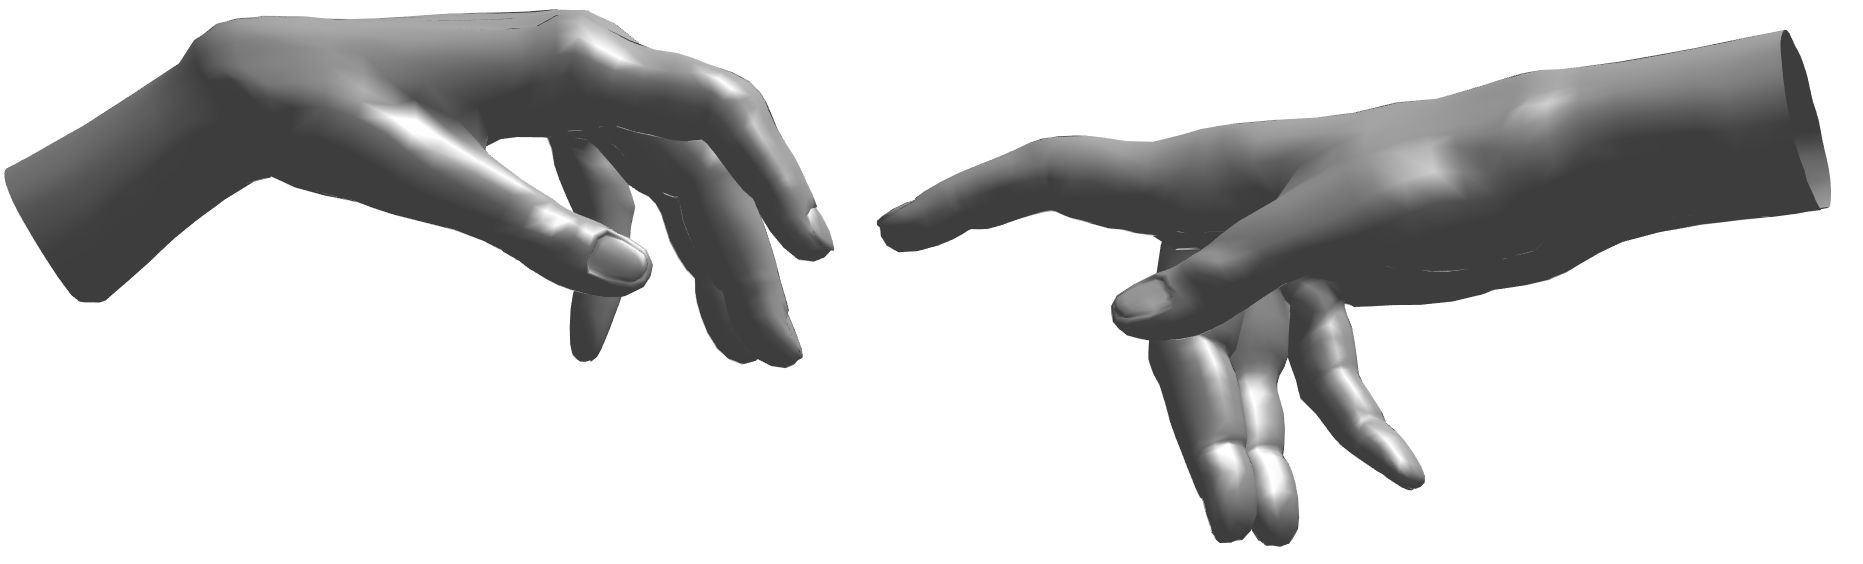
\includegraphics[width=\textwidth]{figs/title}
\end{center}

% Abstract
\rule{\linewidth}{0.4pt}
\begin{center}
\begin{minipage}{0.9\linewidth}
\textbf{Abstract} \\
\emph{%
  Mesh deformation is a common problem in 3D rendering and animation.
  While standard approaches like linear blending or dual quaternion skinning provide high performances, they fail to mimic realistic behaviors.
  On the other hand, physics-based simulations are not suited for real-time tasks, despite giving high quality results.
  Rodolphe Vaillant proposes in his thesis a novel way to adjust errors introduced by approximations during the skinning process.
  Using signed distance functions, his implicit skinning technique fixes and improves bulges.
  This method is well suited for body animation, hand and fingers in particular.
  We have studied and implemented his paper in MatLab and C++ to provide real-time animation for hand-tracking.
}
\end{minipage}
\end{center}
\rule{\linewidth}{0.4pt}

\begin{multicols}{2}


\section{Introduction}

Animation heavily relies on mesh manipulation and transformation.
As always in engineering, time and quality is a matter of trade-off.
Skeletal animation is a popular solution where the mesh surface is attached to a set of interconnected bones.
By transforming the skeleton into different poses, the animator is able to deform a mesh in an intuitive way.

Each vertex is associated to one or more bones, according to weights defined by the designer.
Traditional skinning techniques combine the rigid transformations of bones to update individual vertices.
As such, vertices locations are independent from each others.
While this independence allows highly parallelized implementation, the global shape may be affected, resulting in unrealistic configurations.
On the other hand, physics-based simulations that are used in offline rendering are computationally too expensive in real-time scenarios.
Many solutions were proposed, involving different interpolation strategies and mesh representations.
They exhibit some limitations that Vaillant resolves with \emph{implicit skinning} \cite{Vaillant:2013}.

The first issue, known as the \emph{candy wrapper effect} due to its twisted shrinkage, is induced by bone rotations.
Similarly, bone bending also introduces volume losses.
While the former is only present in \emph{linear blend skinning}, \emph{dual quaternion skinning} \cite{Kavan:2008} also fails to solve the latter.

\begin{figure}[H]
\centering
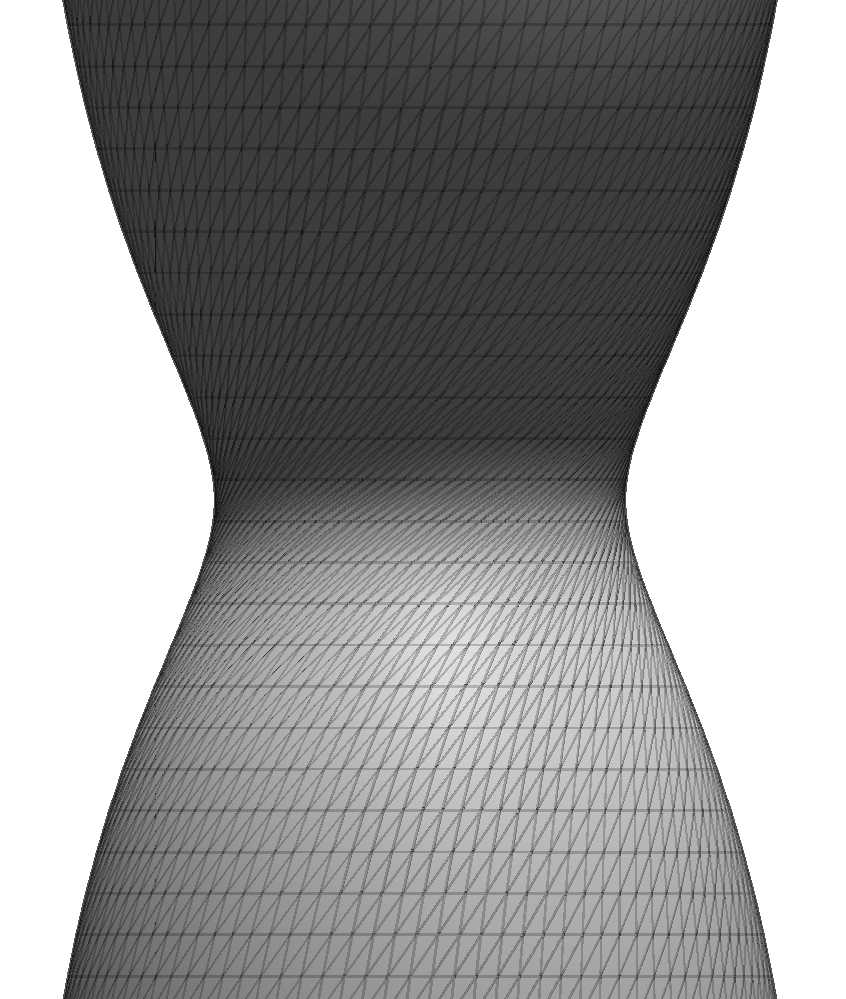
\includegraphics[height=0.15\textheight]{figs/twisted_linear}
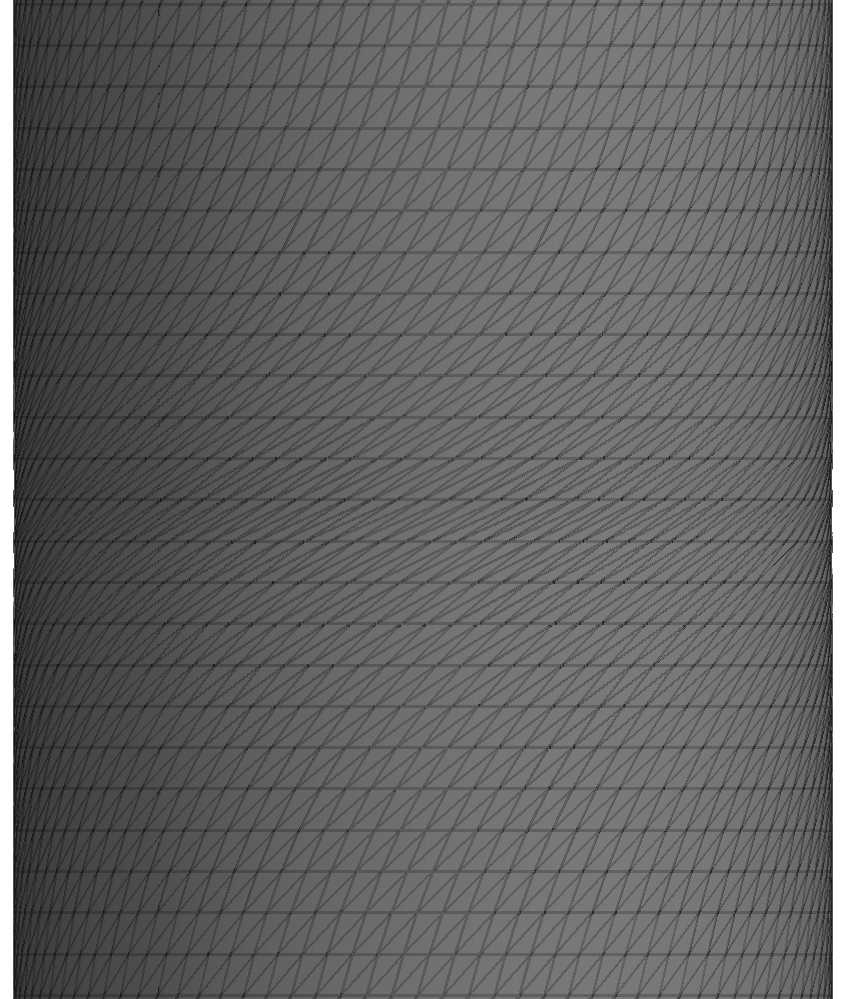
\includegraphics[height=0.15\textheight]{figs/twisted_implicit}
\caption{Illustration of the candy wrapper effect on a twisted cylinder.
Dual quaternion and implicit skinning produce the same transformation (right).}
\end{figure}

\begin{figure}[H]
\centering
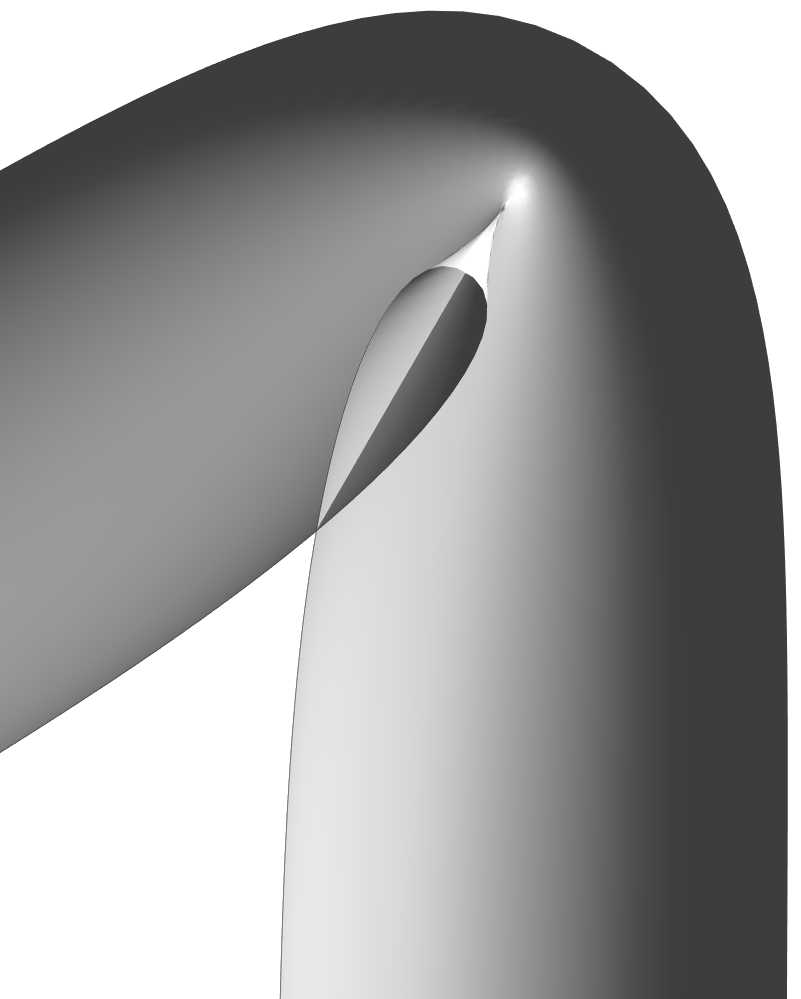
\includegraphics[width=0.15\textwidth]{figs/cylinder_linear}
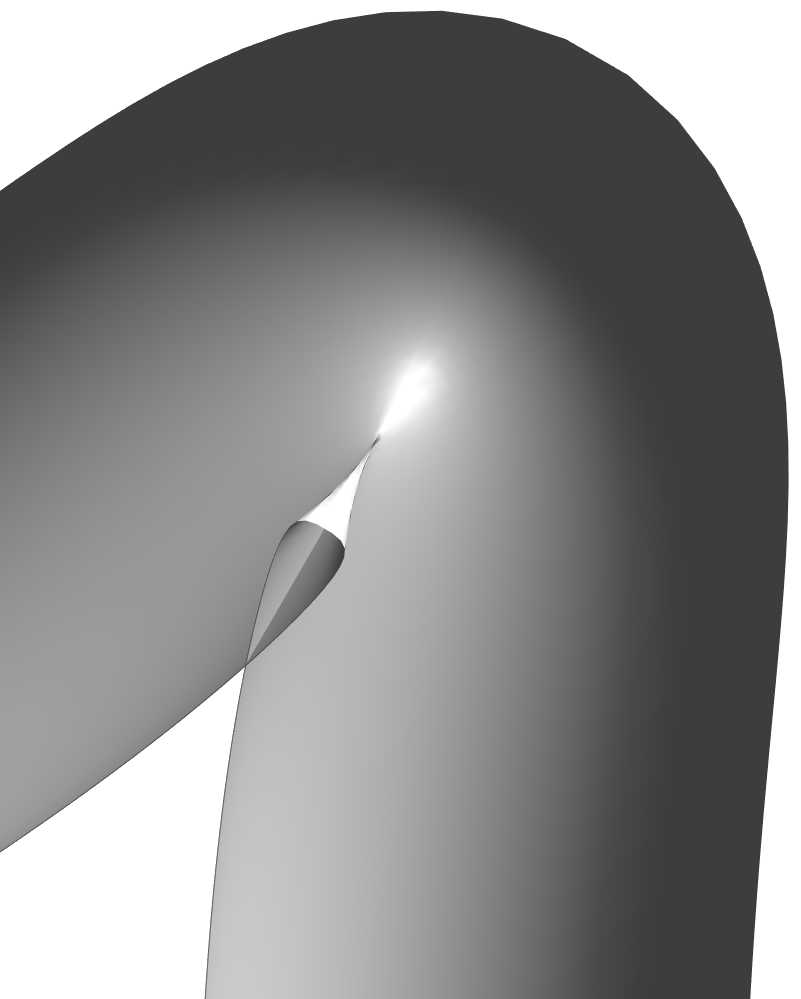
\includegraphics[width=0.15\textwidth]{figs/cylinder_dualquat}
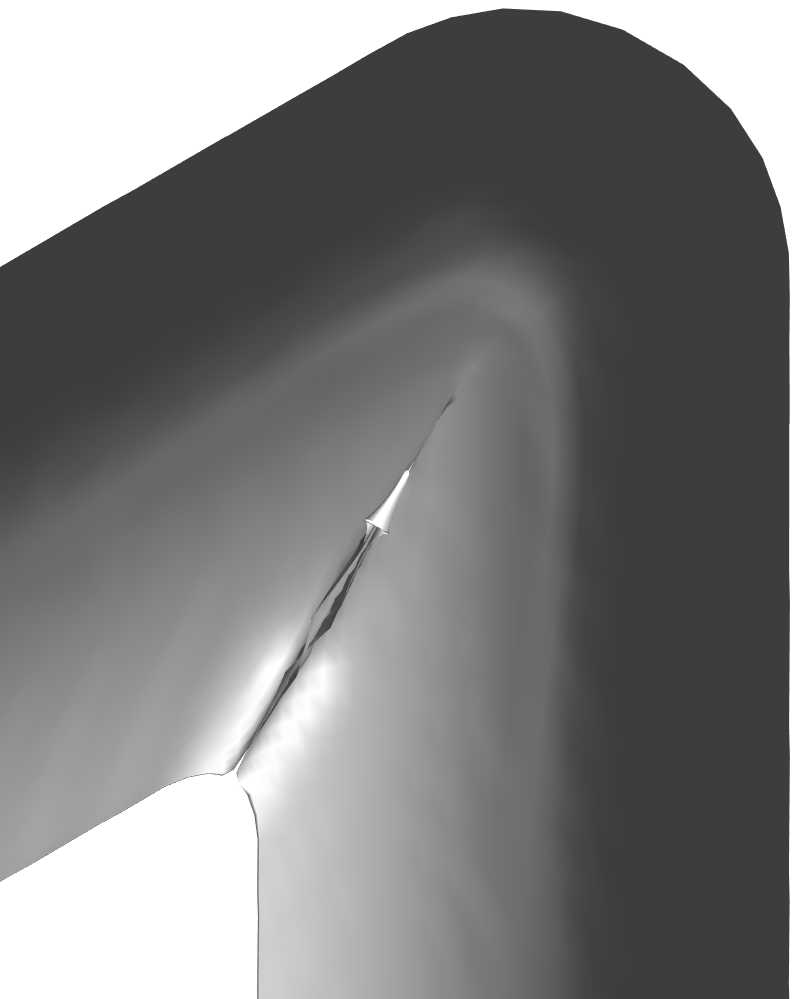
\includegraphics[width=0.15\textwidth]{figs/cylinder_implicit}
\caption{Illustration of the self-intersection problem on a section of a bended cylinder.
Implicit skinning (right) correctly generates a contact region while linear blend skinning (left) and dual quaternion (middle) smoothly fold the mesh.
We can also remark the loss of volume that affects linear blending.}
\end{figure}

Moreover, these methods are unaware of self-intersections.
High deformations, in a realistic scenario, should produce contact regions between skin parts.
By nature, these traditional skinning techniques ignore such a behaviour and produce interleaved surfaces.

Another characteristic of implicit skinning is the ability to produce subtle organic effects.
In particular, we are interested in generating muscular bulges that appear on the skin when fingers bend.
This effect can be seen in figure \ref{fig:compare_skinning} and generate more plausible deformations around joints.

\begin{figure}[H]
\centering
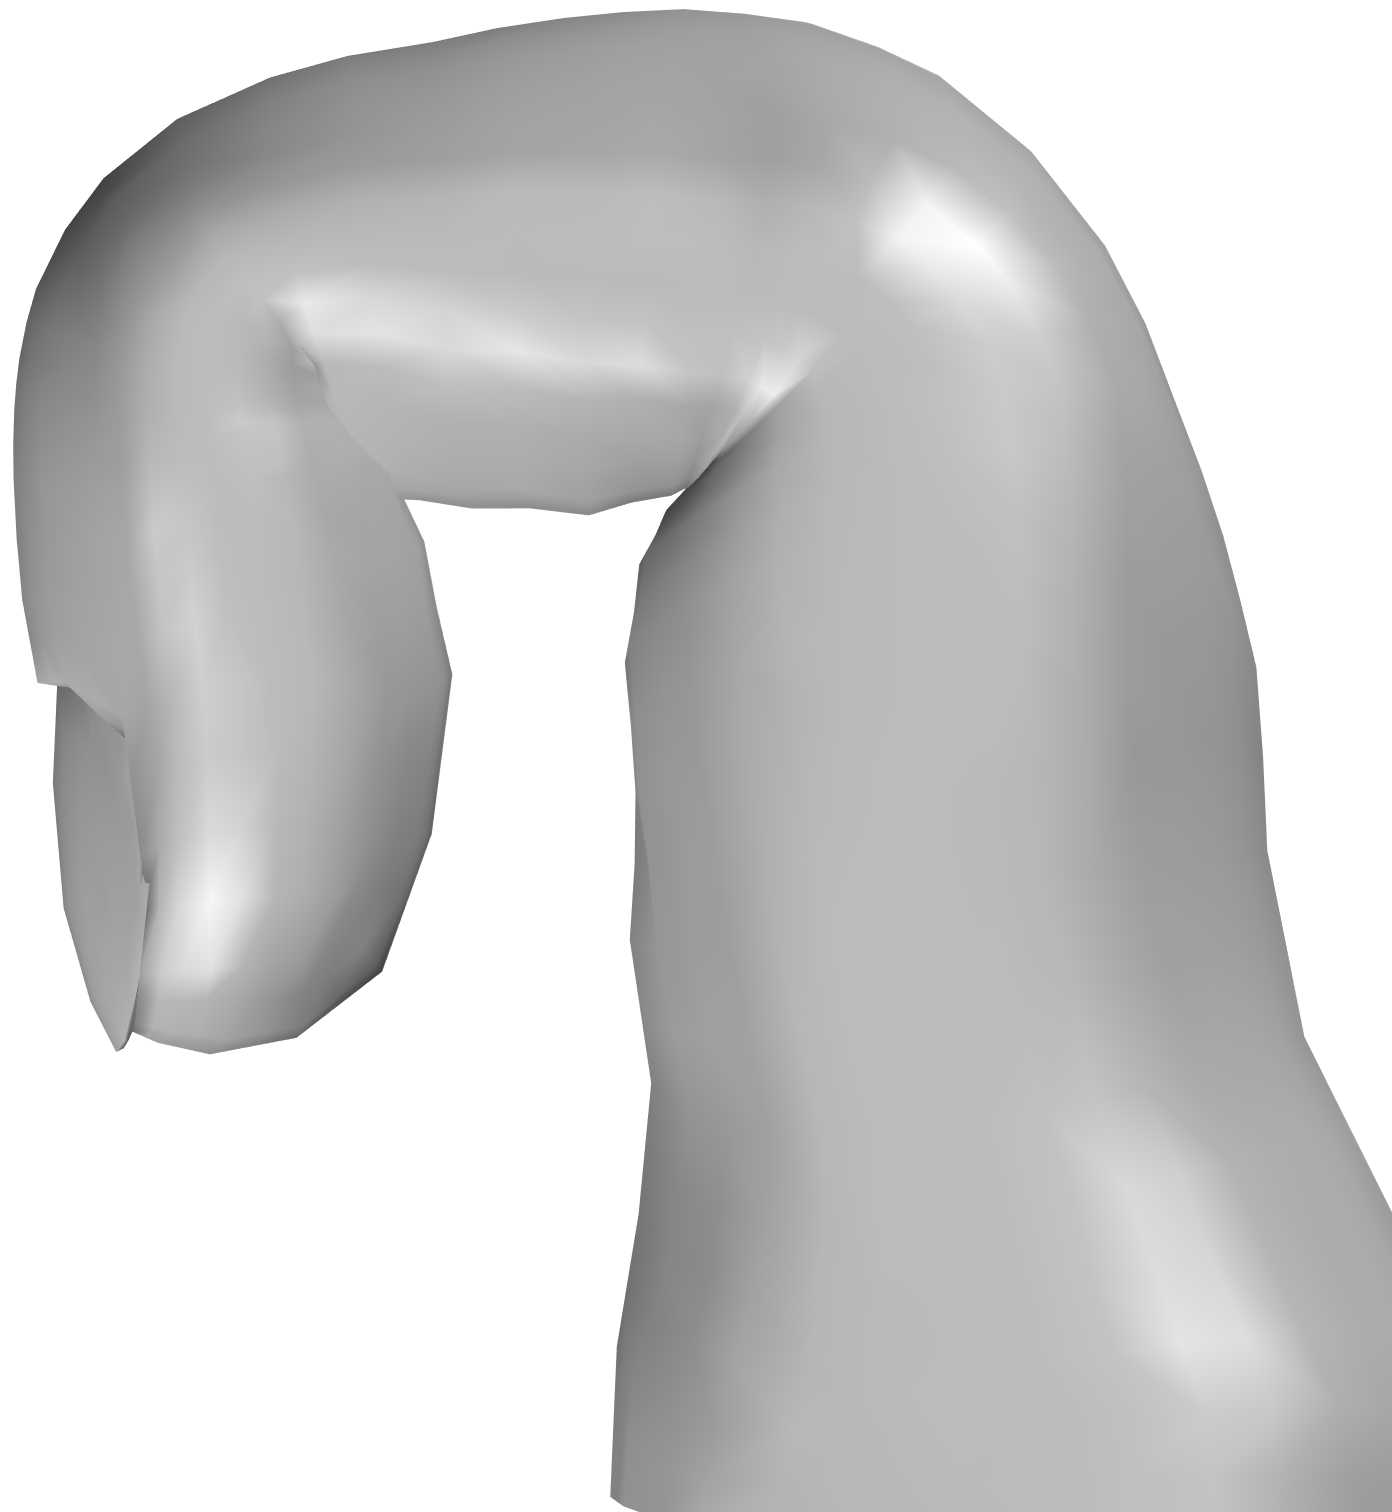
\includegraphics[width=0.15\textwidth]{figs/index_linear}
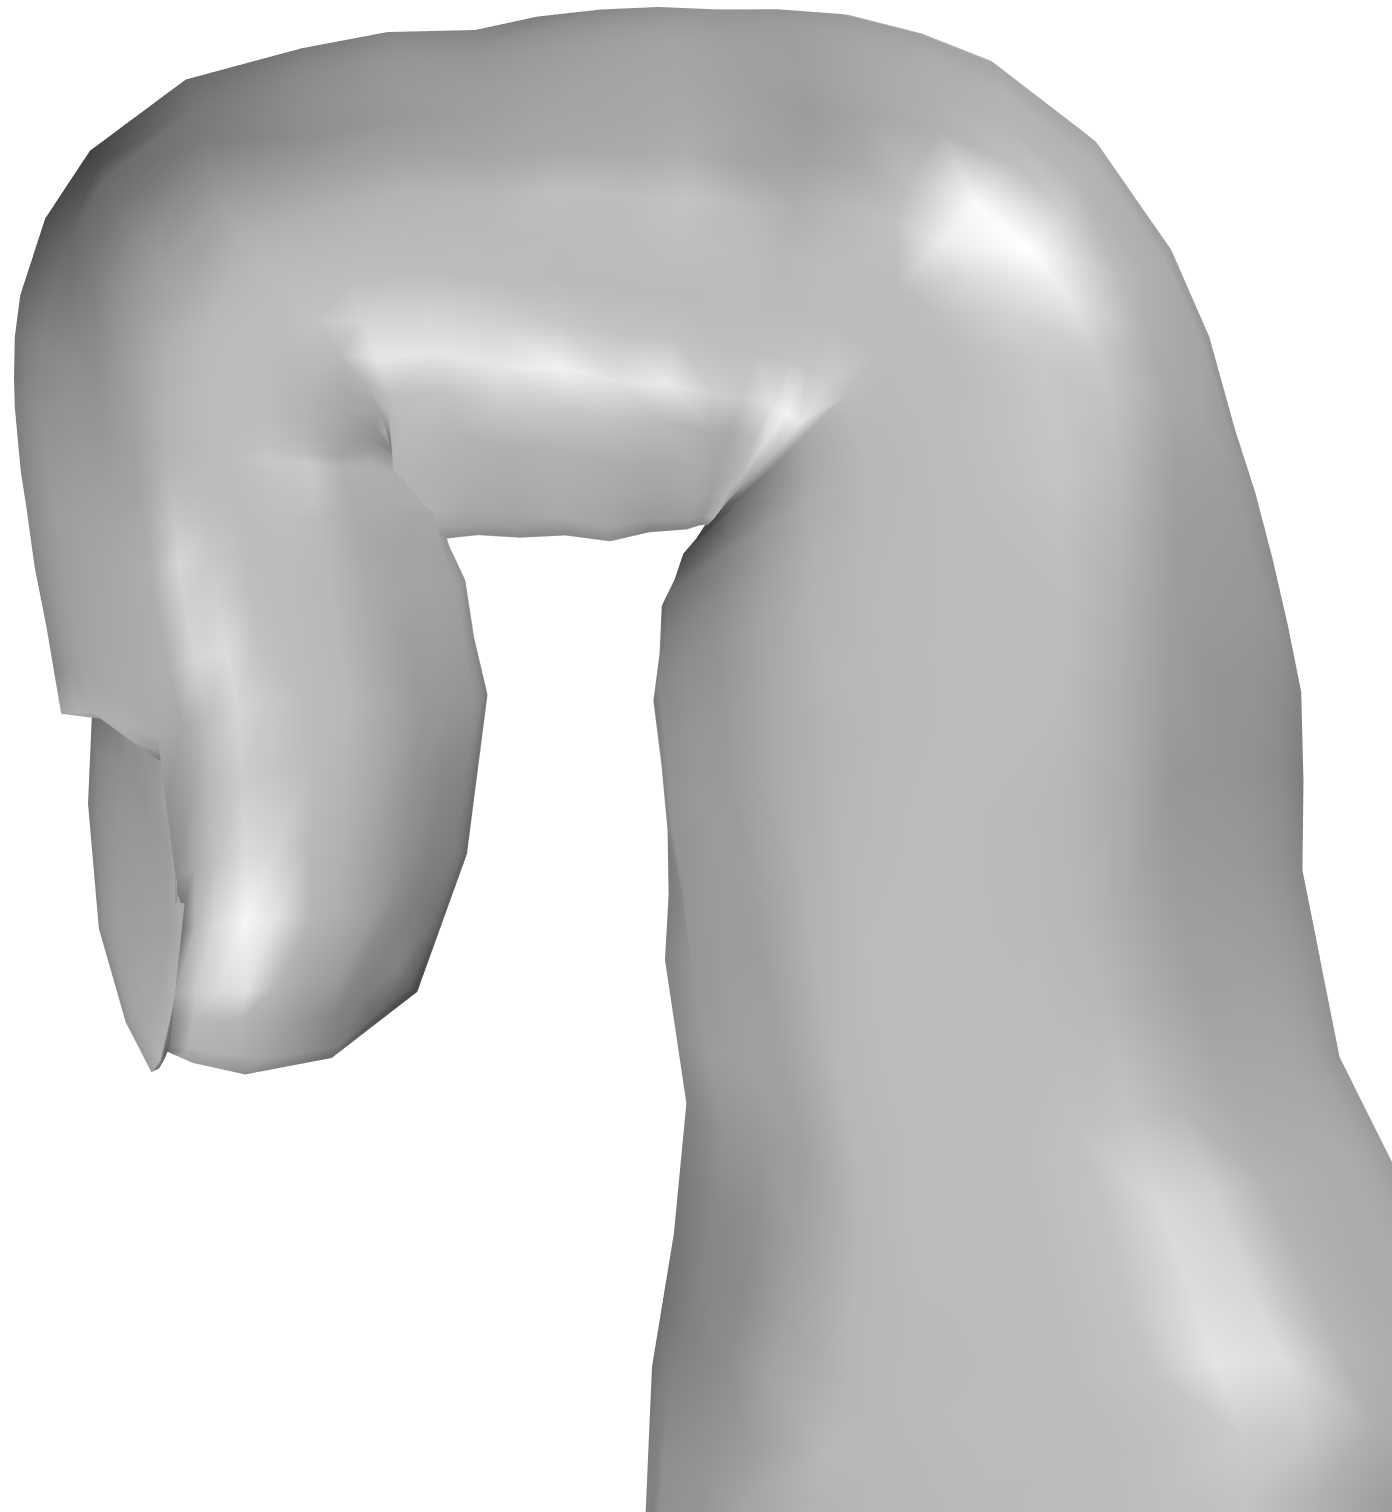
\includegraphics[width=0.15\textwidth]{figs/index_dualquat}
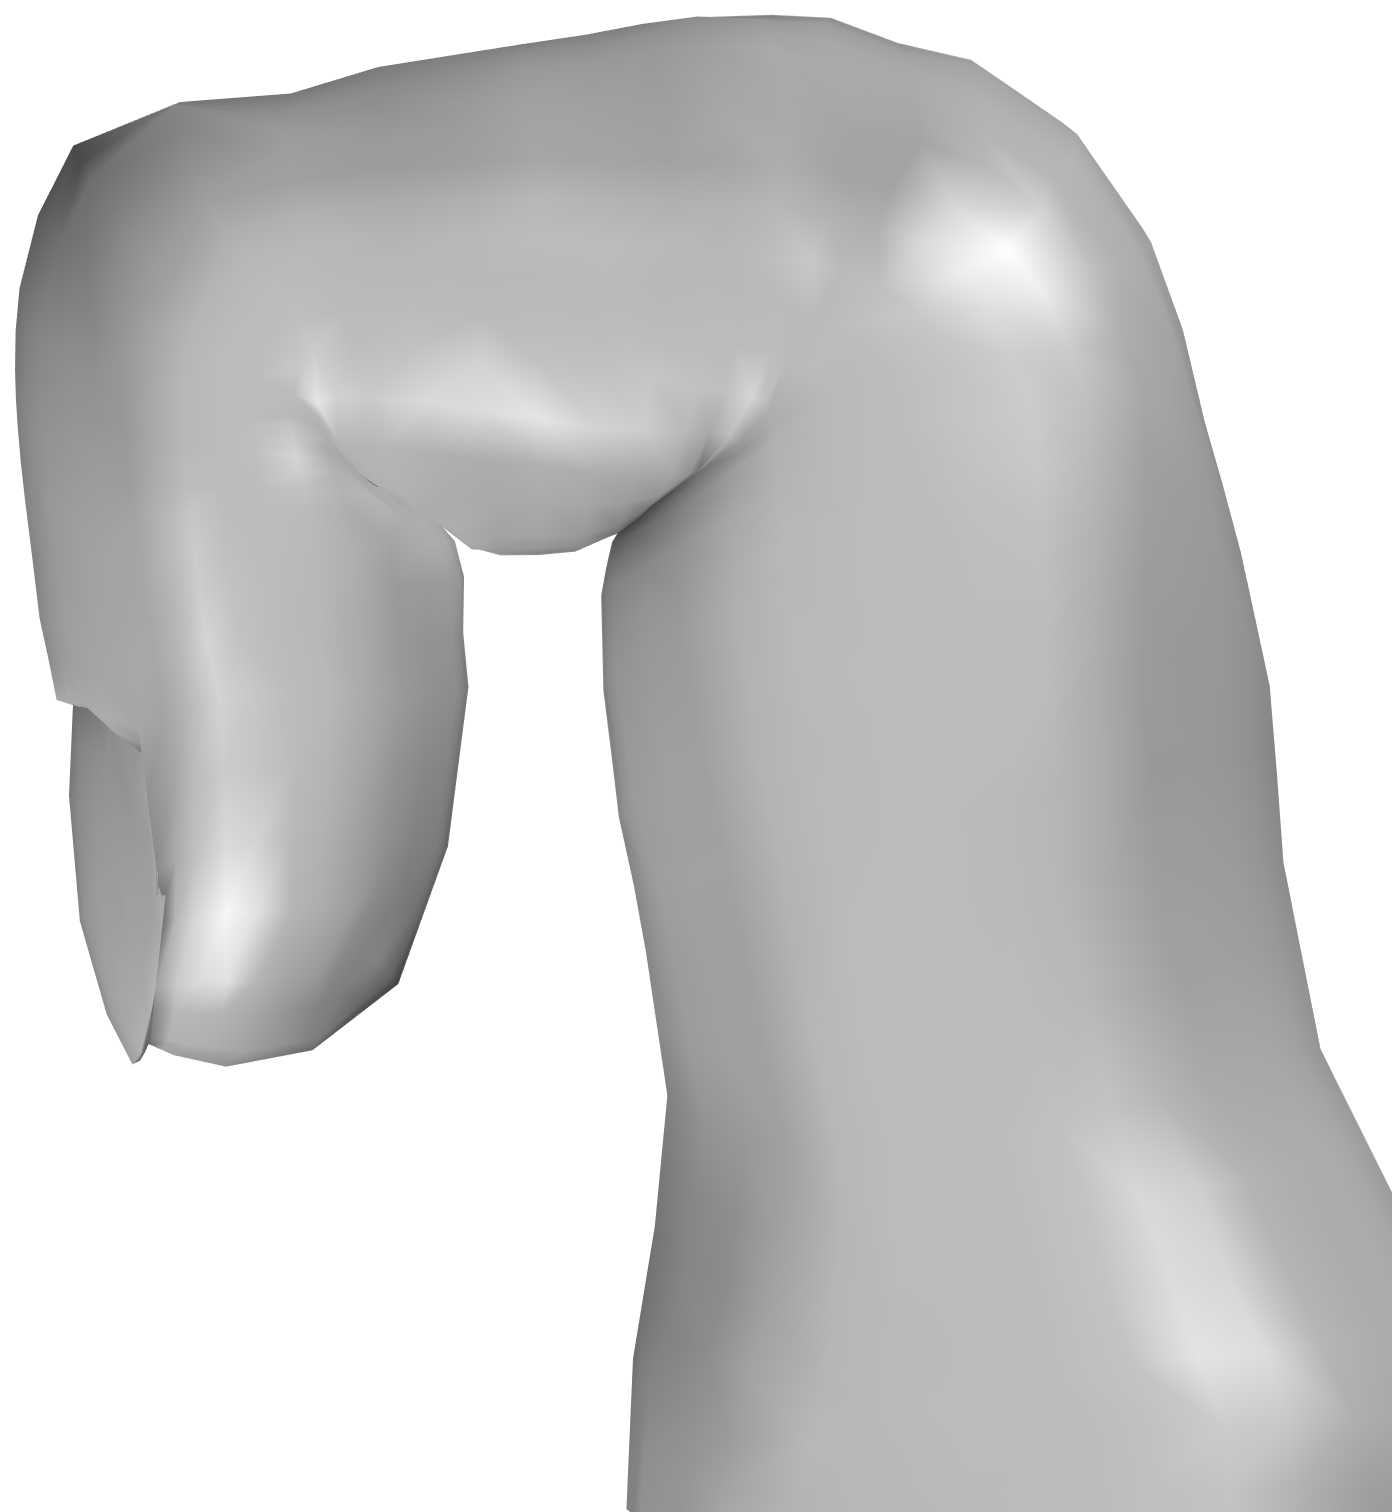
\includegraphics[width=0.15\textwidth]{figs/index_implicit_hrbf}
\caption{An index is bent using linear blending (left), dual quaternion (middle) and implicit skinning (right).
The mesh is composed of $1709$ vertices and $3370$ faces.}
\label{fig:compare_skinning}
\end{figure}


\section{Overview}

We present a study of the implicit skinning algorithm, by Vaillant et al \cite{Vaillant:2013}.
The main work is done using MatLab, in order to produce a clean and as efficient as possible implementation.
In order to provide a performance measure, a C++ version is also available.

In section \ref{section:theory}, we explain in details the theory behind implicit skinning.
Actual results and implementations are discussed in section \ref{section:results}.

As our work is meant to be interfaced with a hand-tracking project, some design constraints are present.
These are discussed in section \ref{section:bone_hierarchy}.
Once the bone structure is defined, traditional skinning techniques are used to provide an initial guess, in \ref{section:traditional}.
This initial guess will be refined and adjusted through implicit skinning.
The idea to prevent volume losses is to track and fix surface movements.

Hence, the first step is to estimate the distance to the bones for each vertex, which is explained in sections \ref{section:mesh_reconstruction} and \ref{section:sdf_composition}.
It is done by building a signed distance field around bones and by combining them into a single function.
This composition is also the key to bulge generation.

Once these building blocks are defined, the actual algorithm is described in section \ref{section:surface_tracking}.
During animation, we apply rigid transformations to the mesh and to the field functions.
The initial guess provided by traditional skinning is iteratively corrected.
Vertices are moved along field gradients until they reach their original distance.
This step, the \emph{surface tracking}, is the core of implicit skinning.
It is also during this stage that self-intersections are detected and handled.

Finally, in section \ref{section:registration}, we discuss an issue related to hand-tracking.
The hand model should match the hand of the user, as poses are highly dependent on bone lengths and volume.
Therefore, some methods are discussed to avoid unnecessary computations.


\section{Theory}
\label{section:theory}

In this section, mathematical details are presented and discussed.
On the other hand, implementation subtleties are omitted for readability, but are available in the commented code.
It should be noted that some mathematical notations about linear algebra and dual quaternion are defined in the appendices \ref{section:calculus} and \ref{section:quaternion}.


\subsection{Bone hierarchy}
\label{section:bone_hierarchy}

In order to animate a hand, a bone hierarchy must be defined.
While following the biological skeleton is an obvious choice for fingers, carpals and metacarpals do not correspond to actual degrees of freedom.
Some bending is allowed to bring the thumb and the pinky closer, which must be modeled.
As a trade-off, we decided to split the palm in half.

Moreover, this project is associated to hand tracking and must interface smoothly with the computer vision algorithm.
More precisely a model-based registration algorithm is used to track user movements.
The hand pose is tracked using spheres as control points, which serve as inputs for our animation rendering.
Hence, our bone design choice is closely related to the spheres placement.
Since the skinning rig only allows rigid deformations, this may also guarantee realistic motion even if some spheres are inaccurately tracked.

In any case, this choice does not affect the remaining pipeline.
As long as bone centers and vertices skinning weights are properly defined, the implicit skinning method does not depend on any particular topology.
While several techniques exist to automatically compute weights, this critical step requires manual adjustments.
Automatic weighting algorithms indeed provide a good guess, but some parts of the palm and thumb ends up with unrealistic weights.

\begin{figure}[H]
\centering
\begin{tikzpicture}
\draw [gray] plot [smooth] coordinates {
(2.61, 0)
(2.54, 1.39)
(2.56, 2.24)
(2.44, 2.58)
(1.18, 4.21)
(0.89, 4.89)
(0.64, 5.67)
(0.44, 6.63)
(0.15, 7.21)
(0.14, 7.57)
(0.35, 7.72)
(0.67, 7.71)
(1.14, 7.38)
(1.38, 6.93)
(1.46, 6.68)
(1.47, 6.46)
(1.83, 5.75)
(1.99, 5.65)
(2.13, 5.92)
(2.46, 6.63)
(2.54, 7.25)
(2.53, 7.74)
(2.46, 8.38)
(2.44, 8.83)
(2.39, 9.49)
(2.39, 10.21)
(2.4, 10.88)
(2.51, 11.26)
(2.86, 11.46)
(3.14, 11.32)
(3.24, 11.01)
(3.28, 10.11)
(3.36, 9.47)
(3.44, 8.97)
(3.56, 8.46)
(3.57, 7.9)
(3.64, 7.74)
(3.79, 7.74)
(3.85, 7.9)
(3.86, 8.58)
(3.97, 9.13)
(4.01, 9.78)
(4.08, 10.51)
(4.21, 11.56)
(4.47, 11.83)
(4.85, 11.78)
(5, 11.5)
(4.97, 10.4)
(4.94, 9.36)
(4.9, 8.88)
(4.89, 8.54)
(4.81, 7.78)
(4.83, 7.67)
(4.92, 7.82)
(5.01, 8.28)
(5.13, 8.68)
(5.26, 9.61)
(5.4, 10.69)
(5.65, 10.96)
(5.97, 10.92)
(6.15, 10.64)
(6.13, 9.89)
(6.07, 9.56)
(6, 8.36)
(5.75, 7.18)
(5.75, 6.96)
(5.83, 6.85)
(5.94, 6.9)
(6.46, 7.88)
(6.63, 8.43)
(6.74, 8.99)
(6.9, 9.29)
(7.19, 9.36)
(7.39, 9.19)
(7.42, 8.93)
(7.36, 8.35)
(7.24, 7.96)
(7.13, 7.43)
(6.83, 6.61)
(6.65, 6.14)
(6.63, 5.93)
(6.44, 5.28)
(6.26, 4.38)
(5.94, 3.11)
(5.72, 2.44)
(5.72, 2.17)
(5.78, 1.65)
(5.86, 0)
};
\draw [gray] (7.11, 9.03) circle (0.32);
\draw [gray] (6.89, 8.08) circle (0.38);
\draw [gray] (6.61, 7.26) circle (0.43);
\draw [gray] (6.19, 6.36) circle (0.51);
\draw [gray] (5.76, 10.57) circle (0.39);
\draw [gray] (5.65, 9.57) circle (0.4);
\draw [gray] (5.56, 8.54) circle (0.44);
\draw [gray] (5.25, 7.22) circle (0.5);
\draw [gray] (4.58, 11.46) circle (0.4);
\draw [gray] (4.51, 10.38) circle (0.43);
\draw [gray] (4.44, 9.18) circle (0.47);
\draw [gray] (4.29, 7.5) circle (0.51);
\draw [gray] (2.82, 11.06) circle (0.4);
\draw [gray] (2.83, 10.03) circle (0.44);
\draw [gray] (2.94, 8.96) circle (0.51);
\draw [gray] (3.07, 7.5) circle (0.54);
\draw [gray] (0.64, 7.28) circle (0.47);
\draw [gray] (1.06, 6.15) circle (0.53);
\draw [gray] (1.74, 4.67) circle (0.72);
\draw [gray] (3.01, 3.28) circle (0.92);
\draw [gray] (2.54, 5.47) circle (0.54);
\draw [gray] (4.15, 2.64) circle (0.79);
\draw [gray] (5.13, 3.01) circle (0.74);
\draw [gray] (5.18, 2.15) circle (0.54);
\draw [gray] (3.11, 2.17) circle (0.56);
\draw [gray] (5.14, 0.64) circle (0.68);
\draw [gray] (3.67, 0) ++ (-5:1.06) arc (-5:185:1.06);
\node [gray] at (6.85, 8.86) {$1$};
\node [gray] at (6.64, 7.97) {$2$};
\node [gray] at (6.32, 7.14) {$3$};
\node [gray] at (5.89, 6.22) {$4$};
\node [gray] at (5.51, 10.4) {$5$};
\node [gray] at (5.43, 9.42) {$6$};
\node [gray] at (5.31, 8.36) {$7$};
\node [gray] at (4.97, 7.04) {$8$};
\node [gray] at (4.35, 11.28) {$9$};
\node [gray] at (4.25, 10.19) {$10$};
\node [gray] at (4.21, 8.97) {$11$};
\node [gray] at (4.01, 7.29) {$12$};
\node [gray] at (2.56, 10.89) {$13$};
\node [gray] at (2.58, 9.85) {$14$};
\node [gray] at (2.69, 8.69) {$15$};
\node [gray] at (2.81, 7.25) {$16$};
\node [gray] at (0.4, 7.08) {$17$};
\node [gray] at (0.81, 5.88) {$18$};
\node [gray] at (1.39, 4.29) {$19$};
\node [gray] at (2.53, 2.93) {$20$};
\node [gray] at (2.54, 5.47) {$21$};
\node [gray] at (4.43, 2.18) {$22$};
\node [gray] at (5.13, 3.01) {$23$};
\node [gray] at (5.18, 2.15) {$24$};
\node [gray] at (3.11, 2.17) {$25$};
\node [gray] at (5.14, 0.64) {$26$};
\node [gray] at (3.67, 0) {$27$};
\node (B18) at (6.89, 8.08) {$18$};
\node (B17) at (6.61, 7.26) {$17$};
\node (B16) at (6.19, 6.36) {$16$};
\node (B14) at (5.65, 9.57) {$14$};
\node (B13) at (5.56, 8.54) {$13$};
\node (B12) at (5.25, 7.22) {$12$};
\node (B11) at (4.51, 10.38) {$11$};
\node (B10) at (4.44, 9.18) {$10$};
\node (B9) at (4.29, 7.5) {$9$};
\node (B8) at (2.83, 10.03) {$8$};
\node (B7) at (2.94, 8.96) {$7$};
\node (B6) at (3.07, 7.5) {$6$};
\node (B5) at (1.06, 6.15) {$5$};
\node (B4) at (1.74, 4.67) {$4$};
\node (B3) at (3.01, 3.28) {$3$};
\node (B2) at (4.15, 2.64) {$2$};
\node (B15) at (5.05, 5.03) {$15$};
\node (B1) at (4.41, 0.32) {$1$};
\draw [dashed] (4.45, 0) -- (B1) -- (B2) -- (B3) -- (B4) -- (B5) -- (0.64, 7.28);
\draw [dashed] (B2) -- (B6) -- (B7) -- (B8) -- (2.82, 11.06);
\draw [dashed] (B2) -- (B9) -- (B10) -- (B11) -- (4.58, 11.46);
\draw [dashed] (B2) -- (B12) -- (B13) -- (B14) -- (5.76, 10.57);
\draw [dashed] (B2) -- (B15) -- (B16) -- (B17) -- (B18) -- (7.11, 9.03);
\end{tikzpicture}
\caption{Schema of control spheres (in gray) and bone hierarchy (in black).}
\end{figure}


\subsection{Traditional skinning}
\label{section:traditional}

By traditional, we refer to common real-time techniques used in animation.
More precisely, \emph{linear blend skinning} and \emph{dual quaternion skinning} \cite{Kavan:2008} were applied to provide the initial guess required by implicit skinning.
Both methods use the skinning weights $w_{b,i}$ associated to each bone $b$ and each vertex $i$.
We compute the transformation $\mathbf{T}_i$ of a vertex as a function of $\mathbf{T}_b$ and $\mathbf{d}_b$, which are respectively the matrix and dual quaternion representing the transformation of the bone $b$.

\begin{equation*}
\mathbf{T}_i = \sum_b w_{b,i} \mathbf{T}_b
\qquad
\mathbf{d}_i = \overbar{\sum_b w_{b,i} \mathbf{d}_b}
\end{equation*}

While $\mathbf{T}_i$ is a $4\times 4$ rigid transformation matrix, $\mathbf{d}_i$ is a \emph{dual quaternion}, which are discussed in appendix \ref{section:quaternion}.
In both case, vertices $\mathbf{v}_i$ and their normals $\mathbf{n}_i$ can be computed independently:

\begin{equation*}
\begin{bmatrix}\mathbf{v}_i' \\ 1 \end{bmatrix} = \mathbf{T}_i \begin{bmatrix} \mathbf{v}_i \\ 1 \end{bmatrix}
\qquad
\begin{bmatrix}\mathbf{n}_i' \\ 0 \end{bmatrix} = \left(\mathbf{T}_i^{-1}\right)^{\mathsf{T}} \begin{bmatrix} \mathbf{n}_i \\ 0 \end{bmatrix}
\end{equation*}

\begin{equation*}
\hat{\mathbf{v}}_i' = \mathbf{d}_i \hat{\mathbf{v}}_i \mathbf{d}_i^*
\qquad
\hat{\mathbf{n}}_i' = \mathbf{d}_{ri} \hat{\mathbf{n}}_i \mathbf{d}_{ri}^*
\end{equation*}
%\begin{equation*}
%\begin{bmatrix}1 \\ \mathbf{0} \end{bmatrix} + \begin{bmatrix}0 \\ \mathbf{v}_i' \end{bmatrix} \varepsilon = \mathbf{d}_i \left(\begin{bmatrix} 1 \\ \mathbf{0} \end{bmatrix} + \begin{bmatrix} 0 \\ \mathbf{v}_i \end{bmatrix} \varepsilon\right) \mathbf{d}_i^*
%\end{equation*}
%\begin{equation*}
%\begin{bmatrix}1 \\ \mathbf{0} \end{bmatrix} + \begin{bmatrix}0 \\ \mathbf{n}_i' \end{bmatrix} \varepsilon = \mathbf{d}_{ri} \left(\begin{bmatrix}1 \\ \mathbf{0} \end{bmatrix} + \begin{bmatrix} 0 \\ \mathbf{n}_i \end{bmatrix} \varepsilon\right) \mathbf{d}_{ri}^*
%\end{equation*}


\subsection{Mesh reconstruction}
\label{section:mesh_reconstruction}

The main idea behind implicit skinning is to adjust positions computed using traditional skinning methods.
More precisely, each vertex is moved to reach its original distance to the bones.
Hence, we need an efficient way to compute a distance for each point in space with respect to each bone.

A \emph{global distance function} $d(\mathbf{p})$ for the surface $\mathcal{S}$ is a \emph{signed distance function} such that $d(\mathbf{p})=0$ if and only if $\mathbf{p}\in \mathcal{S}$.
Moreover, $d(\mathbf{p})<0$ holds for any point inside the surface.
Using such representation, any point $\mathbf{p}$ can be evaluated and moved along the gradient $\frac{\partial}{\partial \mathbf{p}} d$ until it reaches the desired distance.


\subsubsection{Hermite Radial Basis Function}
\label{section:hrbf}

\emph{Radial Basis Function} is a surface reconstruction technique widely used in computer graphics.
As Vaillant proposes in \emph{Implicit Skinning}\cite{Vaillant:2013}, we use \emph{Hermite RBF} \cite{Macedo:2009:HII:1729646.1730288} to compute the signed distance function.

Assuming $m$ centers $\mathbf{c}_k$ and their coefficients $\alpha_i$ and $\boldsymbol\beta_k$, the HRBF distance at $\mathbf{p}$ is defined as:

\begin{equation*}
d(\mathbf{p}) = \sum_{k=1}^m \left(\alpha_k \phi\left( \left\| \boldsymbol\delta_k \right\| \right) +
\boldsymbol\beta_k^T \phi' \left( \left\| \boldsymbol\delta_k \right\| \right) \overbar{\boldsymbol\delta}_k \right)
\end{equation*}

where $\boldsymbol\delta_k = \mathbf{p} - \mathbf{c}_k$.
The notation $\overbar{\mathbf{v}}$ is used to represent the normalized vector $\mathbf{v}$.
Some notations and general relations are described in appendix \ref{section:calculus}.
The gradient, which will be used during vertex projection, is therefore computed as:

\begin{equation*}
\begin{split}
\frac{\partial}{\partial \mathbf{p}} d(\mathbf{p}) &
= \sum_{k=1}^m \left(\alpha_k \phi'\left( \left\| \boldsymbol\delta_k \right\| \right) \overbar{\boldsymbol\delta}_k +
\boldsymbol\beta_k \frac{\phi'\left( \left\| \boldsymbol\delta_k \right\| \right)}{\left\| \boldsymbol\delta_k \right\|} + \right. \\
& \left. \boldsymbol\beta_k^T \overbar{\boldsymbol\delta}_k \left( \phi'' \left( \left\| \boldsymbol\delta_k \right\| \right) \overbar{\boldsymbol\delta}_k - \phi'\left( \left\| \boldsymbol\delta_k \right\| \right) \frac{\overbar{\boldsymbol\delta}_k}{\left\| \boldsymbol\delta_k \right\|} \right) \right)
\end{split}
\end{equation*}

A simple yet efficient kernel $\phi$ is the \emph{triharmonic} function:

\begin{equation*}
\phi(x) = x^3 \qquad
\phi'(x) = 3x^2 \qquad
\phi''(x) = 6x
\end{equation*}

Hence, the simplified HRBF formulas are:

\begin{equation*}
d(\mathbf{p}) = \sum_{k=1}^m \left(\alpha_k \left\| \boldsymbol\delta_k \right\|^3 + 3\left\| \boldsymbol\delta_k \right\| \boldsymbol\beta^T \boldsymbol\delta_k \right)
\end{equation*}

\begin{equation*}
\frac{\partial}{\partial \mathbf{p}} d(\mathbf{p}) = 3\sum_{k=1}^m \left(\alpha_k \left\| \boldsymbol\delta_k \right\| \boldsymbol\delta_k +
\boldsymbol\beta_k^T \overbar{\boldsymbol\delta}_k \boldsymbol\delta_k +
\left\| \boldsymbol\delta_k \right\| \boldsymbol\beta_k \right)
\end{equation*}

The coefficients are usually computed with an optimization problem, to fit known points on the surface.
Given $n$ points $\mathbf{v}_i$ and their normals $\mathbf{n}_i$, the HRBF should represent them as precisely as possible.
Therefore, we should satisfy the following equations, which gives a linear system with $4n$ equations and $4m$ variables:

\begin{equation*}
d(\mathbf{v}_i) = 0 \qquad \nabla d(\mathbf{v}_i) = \mathbf{n}_i \qquad \forall i
\end{equation*}

The choice of centers and control points is arbitrary and is the key to proper HRBF reconstruction.
As Vaillant suggests, we use Poisson sampling over the surface.
In order to automatically handle joints, we use an ad hoc hole filling method based on convex optimization (which is discussed in appendix \ref{section:quadratic}).
Each hole $\mathcal{H}$ is patched with a regular grid of average valence of 6, which is then inflated.
The following convex program is used to tightly fit the patch and minimize the distance between vertices:

\begin{equation*}
\begin{aligned}
& \underset{\mathbf{v}}{\text{minimize}} & & \sum_{(i, j)} \left\| \mathbf{v}_i - \mathbf{v}_j \right\|_2^2 \\
& \text{subject to} & & \mathbf{v}_h = \mathbf{v}_h^* \qquad h \in \mathcal{H},
\end{aligned}
\end{equation*}
where $\mathbf{v}_h^*$ are the vertices on the boundary of $\mathcal{H}$.


\subsubsection{Spherical primitives}

Another approach to signed distance functions relies on approximations by primitives composition.
Spheres are a common choice when it comes to simple geometrical objects.
Intuitively, the distance and gradient of a sphere of center $\mathbf{c}$ and radius $r$ are given by:

\begin{equation*}
d(\mathbf{p}) = \left\| \mathbf{p} - \mathbf{c} \right\| - r
\end{equation*}

\begin{equation*}
\frac{\partial}{\partial \mathbf{p}} d(\mathbf{p}) = \overbar{\mathbf{p} - \mathbf{c}}
\end{equation*}

To properly approximate fingers, a cylindrical shape is required.
We call \emph{bisphere} the convex hull of two spheres.
This can be seen as two distinct spheres connected by a truncated cone.
To compute the distance and gradient, we need to determine on which part the projection $p'$ lies.

\begin{figure}[H]
\centering
\begin{tikzpicture}
\coordinate [label = {below left:$\mathbf{c}_1$}] (c1) at (0, 0);
\coordinate [label = {below right:$\mathbf{c}_2$}] (c2) at (5, 0);
\coordinate (x) at (1, 0);
\coordinate (y) at (0, 1);
\coordinate (t1) at (0.4, 1.9596);
\coordinate (u) at (1.3798, 1.7596);
\coordinate (v) at (0.6, 2.9394);
\coordinate (t2) at (5.2, 0.9798);
\coordinate [label = {right:$\mathbf{p}$}] (p) at (3.5, 2.5);
\coordinate [label = {below:$\mathbf{q}$}] (q) at (3.5, 0);
\coordinate [label = {below:$\mathbf{p}'$}] (pp) at (3.2701, 1.3737);
\coordinate [label = {above:$e$}] (e) at (0.1, 0);
\coordinate (f) at (0.2, 0);
\coordinate (t0) at (-0.8, 2.2045);
\coordinate (t3) at (6, 0.8165);
\draw (0, 0) ++ (-30:2) arc (-30:120:2);
\draw (c2) circle (1);
\draw [->] (c1) -- node [below] {$\mathbf{x}$} (x);
\draw [->] (c1) -- node [left] {$\mathbf{y}$} (y);
\draw [->] (t1) -- node [below] {$\mathbf{u}$} (u);
\draw [->] (t1) -- node [left] {$\mathbf{v}$} (v);
\draw [dashed] (x) -- (c2);
\draw [dashed] (c1) -- node [above left] {$r_1$} (t1);
\draw [dashed] (c2) -- node [left] {$r_2$} (t2);
\draw (u) -- (t2);
\draw [dashed] (p) -- (q);
\draw [dashed] (p) -- node [left] {$d$} (pp);
\draw [dashed] (c2) -- (0.2, 0.9798) -- node [right] {$f$} (f);
\draw [dashed] (t0) -- (t1);
\draw [dashed] (t2) -- (t3);
\end{tikzpicture}
\caption{Schema of a bisphere and relevant metrics used in equations.}
\label{figure:bisphereschema}
\end{figure}

The following derivations are mostly geometrical relations based on figure \ref{figure:bisphereschema}:

\begin{equation*}
\mathbf{x} = \overbar{\mathbf{c}_2 - \mathbf{c}_1}
\qquad
\mathbf{y} = \overbar{\mathbf{p} - \mathbf{q}}
\end{equation*}

\begin{equation*}
\mathbf{q} = \left( \mathbf{c}_1 - \mathbf{p} \right)^T \mathbf{x} \mathbf{x}
\qquad
e = \frac{\left( r_1 - r_2 \right)^2}{\left\| \mathbf{c}_2 - \mathbf{c}_1 \right\|}
\end{equation*}

\begin{equation*}
f = \sqrt{\left(\left\| \mathbf{c}_2 - \mathbf{c}_1 \right\| - e \right) e}
\qquad
\theta = \frac{f}{\left\| \mathbf{c}_2 - \mathbf{c}_1 \right\| - e}
\end{equation*}

\begin{equation*}
\mathbf{u} = \mathbf{x} - \theta \mathbf{y}
\qquad
\mathbf{v} = \mathbf{y} + \theta \mathbf{x}
\end{equation*}

Using $\mathbf{u}$, we can check whether $\mathbf{p}'$ lies on the conical segment, where the gradient and distance are defined by $\mathbf{v}$.
Otherwise, the sphere formulas can be used.

Finally, an additional primitive is needed to represent planar parts, such as the palm.
Following the same idea to extend our model, we call \emph{trisphere} the convex hull defined by three spheres.
Again, we can use the previous formulas for some cases.
If $\mathbf{p}'$ lies on the tangential triangle, then the distance and gradient can be computed using the normal.
Otherwise, values are computed using the right bisphere.

\begin{figure}[H]
\centering
\begin{tikzpicture}
\coordinate [label = {below left:$\mathbf{c}_1$}] (c1) at (0, 0);
\coordinate [label = {below:$\mathbf{c}_2$}] (c2) at (3, 2.5);
\coordinate [label = {below right:$\mathbf{c}_3$}] (c3) at (4.5, 0.5);
\coordinate (s13) at (-0.7522, 1.8531);
\coordinate (s31) at (2.5779, 3.4065);
\coordinate (s23) at (3.8560, 3.0170);
\coordinate (s32) at (5.1420, 0.8877);
\coordinate (s12) at (2.7733, -1.0216);
\coordinate (s21) at (4.7854, -0.1936);
\coordinate [label = {left:$\mathbf{t}_1$}] (t1) at (0.4945, 1.7307);
\coordinate [label = {above right:$\mathbf{t}_2$}] (t2) at (3.2472, 3.3654);
\coordinate [label = {below right:$\mathbf{t}_3$}] (t3) at (4.6854, 1.1490);
\coordinate [label = {right:$\mathbf{p}$}] (p) at (4.4121, 3.4423);
\coordinate [label = {left:$\mathbf{p}'$}] (pp) at (4, 2);
\coordinate (n) at (4.2747, 2.9615);
\draw (0, 0) ++ (-30:2) arc (-30:120:2);
\draw (c2) circle (1);
\draw (c3) circle (0.75);
\draw [dashed] (c1) -- (c2);
\draw [dashed] (c2) -- (c3);
\draw [dashed] (c3) -- (c1);
\draw (t1) -- (t2);
\draw (t2) -- (t3);
\draw (t3) -- (t1);
\draw [dashed] (c1) -- (t1);
\draw [dashed] (c2) -- (t2);
\draw [dashed] (c3) -- (t3);
\draw (s13) -- (s31);
\draw (s23) -- (s32);
\draw (s12) -- (s21);
\draw [dashed] (p) -- (pp);
\draw [->] (pp) -- node [right] {$\mathbf{n}$} (n);
\end{tikzpicture}
\caption{Schema of a trisphere with the upper tangential plane and its normal.}
\end{figure}


\subsection{Composition of distance functions}
\label{section:sdf_composition}

While global distance functions are an intuitive way to represent distances, they have some drawbacks when it comes to combination of multiple surfaces.
More precisely, locality is not easily defined.
A volume should only influence close neighborhood and should not have any effect after some distance.
Hence, we need functions with \emph{local support}, which we call \emph{local distance functions}.

The basic idea is that we define a new function $d$ such that $d(\mathbf{p}) = 1$ inside and $d(\mathbf{p}) = 0$ outside the object, with a smooth transition.
The implicit surface is therefore defined by the $0.5$-isosurface.
As Vaillant suggests, a global distance function can be remapped to provide local support using the following reparametrization, where $l(x)$ is an interpolation function and $r$ is the distance threshold:

\begin{equation*}
t_r(d) = \left\{ \begin{array}{ll}
1 & \mathrm{if\ }d < -r \\
0 & \mathrm{if\ }d > r \\
l(\frac{d}{r}) & \mathrm{otherwise}
\end{array} \right.
\end{equation*}

\begin{equation*}
l(x) = -\frac{3}{16}x^5 + \frac{5}{8}x^3 - \frac{15}{16}x + \frac{1}{2}
\end{equation*}

\begin{figure}[H]
\centering
\begin{tikzpicture}[xscale=2,yscale=1.2]
  \draw[->] (-1.5,0) -- (1.5,0) node[right] {$d$};
  \draw[->] (0,-0.2) -- (0,1.5) node[above] {$t_r(d)$};
  \draw[domain=-1:1,smooth,variable=\x,black] plot ({\x},{-0.1875*\x^5 + 0.625*\x^3 - 0.9375*\x + 0.5});
  \draw[domain=-1.5:-1,smooth,variable=\x,black]  plot ({\x},{1});
  \draw[domain=1:1.5,smooth,variable=\x,black]  plot ({\x},{0});
  \draw  (-1,0) node[anchor=north] {$-r$}
    (1,0) node[anchor=north] {$r$}
    (0,1) node[anchor=east] {$1$};
  \draw[dotted] (-1,0) -- (-1,1.3);
  \draw[dotted] (1,0) -- (1,1.3);
  \draw[-] (-0.05,1) -- (0.05,1);
\end{tikzpicture}
\caption{Plot of the reparametrization function.}
\end{figure}

Using global distance functions, each bone can be reconstructed and reparametrized.
To compute the distance to the whole mesh, a single distance function must be defined.
To combine bone fields, we apply a two steps composition.
First, for each pair of neighboring bones $(i, j)$, we combine the two fields into one $f_{ij} = g_{ij}(f_i, f_j)$ using an \emph{operator}.
Then, the fields $f_{ij}$ are combined into a single function $f$ using the \emph{union operator}.


\subsubsection{Union operator}

An important and yet simple operator is the \emph{union}.
As the name implies, this composition function aims to merge two surfaces together.
Due to the nature of local distance functions, this is achieved in a straightforward manner:

\begin{equation*}
g_u(f_1, f_2) = \max(f_1, f_2)
\end{equation*}

As stated before, the gradient of distance functions is required during surface tracking.
While Gourmel et al. \cite{Gourmel:2013} thoroughly discuss continuity issues by introducing quasi-$C^\infty$ operators to ensure mathematical correctness, we are not going to provide a continuous approximation of the union operator.
In practice, the maximum is implemented by using the largest distance, since the singularity is numerically never reached.

\begin{figure}[H]
\centering
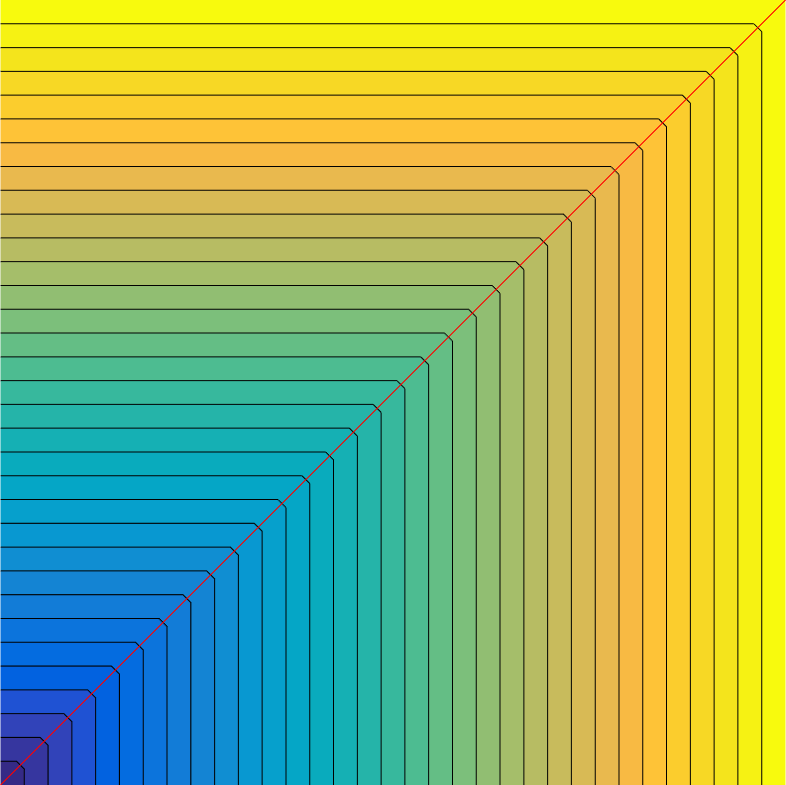
\includegraphics[width=0.22\textwidth]{figs/union_field}
\hfill
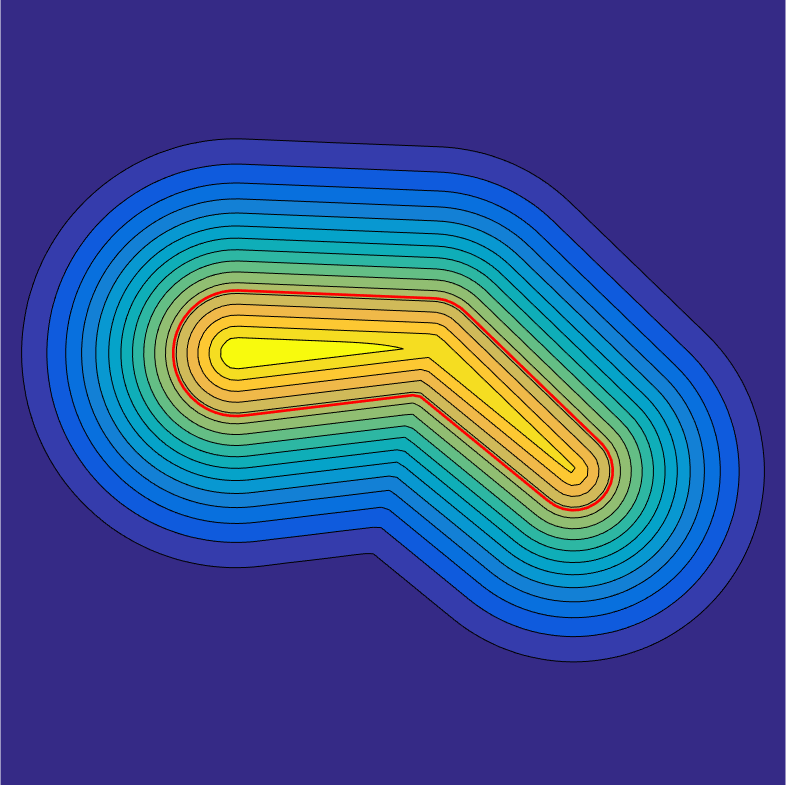
\includegraphics[width=0.22\textwidth]{figs/union_finger}
\caption{Illustration of the union operator on the left, where the axes are $f_1$ and $f_2$.
The red diagonal shows the discontinuity between gradients, which produces the sharp union on the right.
The graph on the left represents how $g_u$ depends on $f_1$ and $f_2$, which are respectively abscissa and ordinate.
Vertical lines are isosurfaces of $f_1$ and horizontal lines are those of $f_2$.
The limits of both axis are $[0, 1]$ since the field functions are compactly supported.}
\end{figure}


\subsubsection{Blend operator}
\label{section:blendoperator}

A major aspect of Vaillant's work is about producing realistic skin behavior.
As the finger bends, the tissue on the inner part of the joint is compressed and produces a bulge.
Hence, another composition function is required, the \emph{blend operator}.

\begin{figure}[H]
\centering
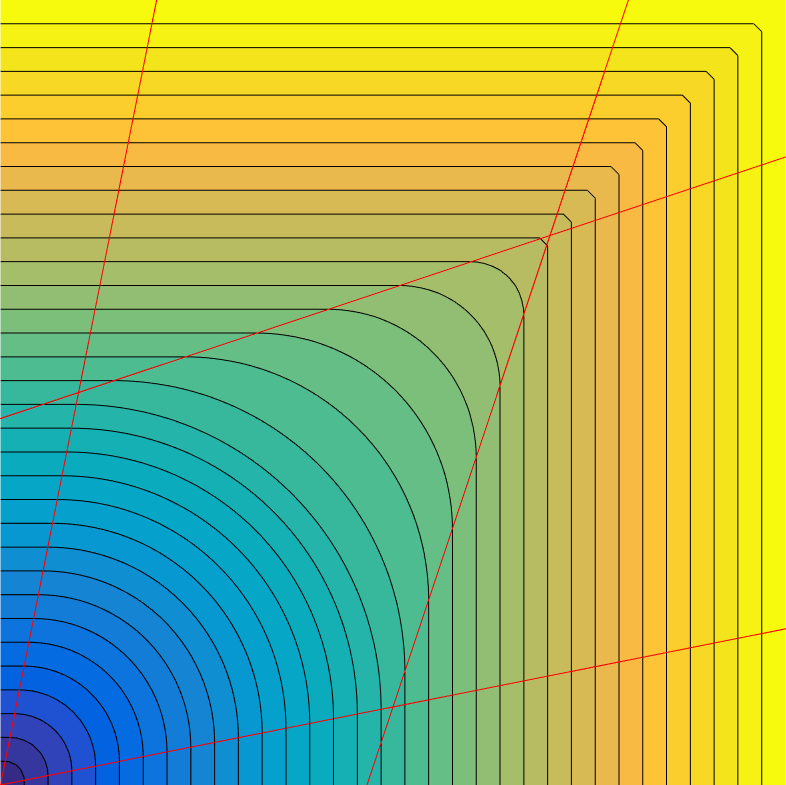
\includegraphics[width=0.22\textwidth]{figs/blend_field}
\hfill
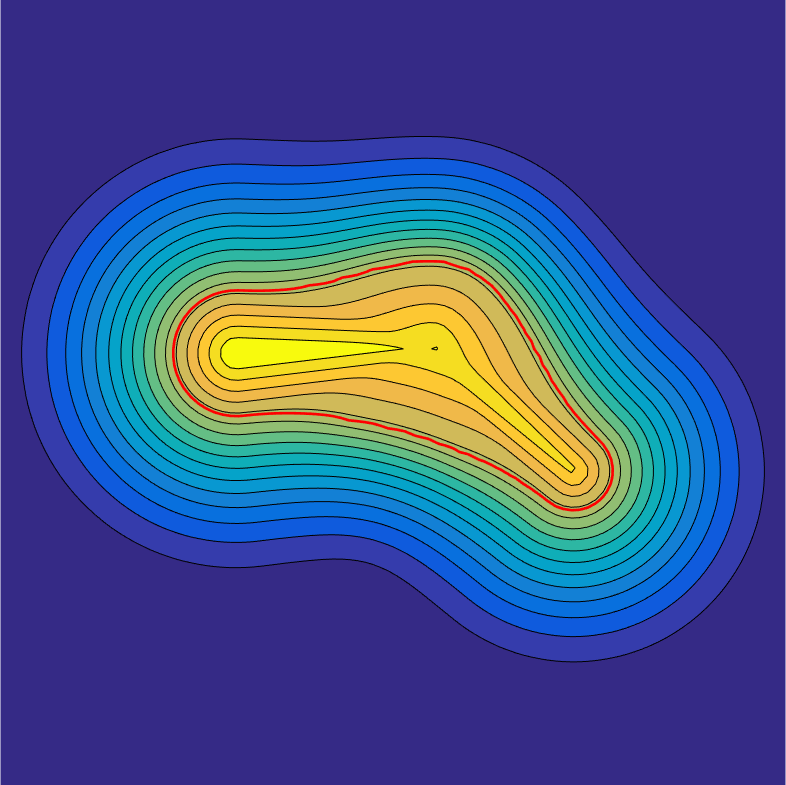
\includegraphics[width=0.22\textwidth]{figs/blend_finger}
\caption{Illustration of the blend operator on the left.
The trapezoidal region produces higher values than the union operator, giving a bulging effect on the right.}
\label{fig:blendop}
\end{figure}

While the behavior is similar to the union for distant configurations, the distance field is increased when both fields are close.
The red lines, which are given by the following equations, delimit the boundary between union and bulging.
They are controlled by a parameter $\theta$, which is the angle of boundary lines.

\begin{equation*}
f_2 = \tan(\theta)f_1 \qquad f_1 = \tan(\theta)f_2
\end{equation*}

\begin{equation*}
f_2 = \frac{1}{2} (7 - 5\tan(\theta))f_1 + \frac{7}{4} (\tan(\theta) - 1)
\end{equation*}

\begin{equation*}
f_1 = \frac{1}{2} (7 - 5\tan(\theta))f_2 + \frac{7}{4} (\tan(\theta) - 1)
\end{equation*}

The two families of curves in the trapezoidal area are given by solving the following equations with respect to $C$:

\begin{equation*}
(f_1 + a + bC)^2 + (f_2 + a + bC)^2 = (C + a + bC)^2
\end{equation*}

\begin{equation*}
a = \left\{ \begin{array}{ll}
  0 & \mathrm{if\ lower\ area} \\
  -\frac{7}{4} (\tan(\theta) - 1) & \mathrm{if\ upper\ area}
\end{array} \right.
\end{equation*}

\begin{equation*}
b = \left\{ \begin{array}{ll}
  -\tan(\theta) & \mathrm{if\ lower\ area} \\
  -\frac{1}{2} (7 - 5\tan(\theta)) & \mathrm{if\ upper\ area}
\end{array} \right.
\end{equation*}

To determine in which area the pair $(f_i, f_j)$ lies, we use the following tests, which are true in the upper area:

\begin{equation*}
\frac{\left( f_1 - \frac{\tan(\theta)}{2} \right)^2 + \left( f_2 - \frac{\tan(\theta)}{2} \right)^2}{\left( \tan(\theta) - \frac{\tan(\theta)}{2} \right)^2} > 1
\end{equation*}

\begin{equation*}
f_1 > \frac{\tan(\theta)}{2}\mathrm{\ or\ }f_2 > \frac{\tan(\theta)}{2}
\end{equation*}

The parameter $\theta$ is used to control the blending strength.
It it usually computed according to the angle $\alpha$, using the following mapping:

\begin{equation*}
\theta(\alpha) = \left\{\begin{array}{ll}
  \theta_0 & \mathrm{if\ }\alpha \leq \alpha_0 \\
  l_0(\alpha) & \mathrm{if\ }\alpha \in \left] \alpha_0, \alpha_1 \right] \\
  l_1(\alpha) & \mathrm{if\ }\alpha \in \left] \alpha_1, \alpha_2 \right] \\
  \theta_2 & \mathrm{if\ }\alpha > \alpha_2 \\
\end{array}\right.
\end{equation*}

\begin{equation*}
l_0(\alpha) = \left( \kappa \left(\frac{\alpha - \alpha_1}{\alpha_0 - \alpha_1}\right)\right)^{\omega_0} (\theta_0 - \theta_1) + \theta_1
\end{equation*}

\begin{equation*}
l_1(\alpha) = \left( \kappa \left(\frac{\alpha - \alpha_1}{\alpha_2 - \alpha_1}\right)\right)^{\omega_1} (\theta_2 - \theta_1) + \theta_1
\end{equation*}

\begin{equation*}
\kappa(x) = 1 - \exp\left( 1 - \frac{1}{1 - \exp(1 - \frac{1}{x})} \right)
\end{equation*}

\begin{figure}[H]
\centering
\begin{tikzpicture}
\draw[->] (0, 0) -- (4, 0);
\draw[->] (0, 0) -- (0, 2);
\draw[gray,dashed] (0.7854, 2) -- (0.7854, 0);
\draw[gray,dashed] (3.1416, 2) -- (3.1416, 0);
\draw[gray,dashed] (0, 1.5708) -- (4, 1.5708);
\draw[gray,dashed] (0, 0.6283) -- (4, 0.6283);
\draw (0.7854, 0.025) -- (0.7854, -0.025) node [below] {$\alpha_0$};
\draw (3.1416, 0.025) -- (3.1416, -0.025) node [below] {$\alpha_1=\alpha_2$};
\draw (0.025, 1.5708) -- (-0.025, 1.5708) node [left] {$\theta_0= \theta_2$};
\draw (0.025, 0.6283) -- (-0.025, 0.6283) node [left] {$\theta_1$};
\draw [blue] plot [smooth] coordinates {
(0, 1.57079632679490)
(0.102564102564103, 1.57079632679490)
(0.205128205128205, 1.57079632679490)
(0.307692307692308, 1.57079632679490)
(0.410256410256410, 1.57079632679490)
(0.512820512820513, 1.57079632679490)
(0.615384615384615, 1.57079632679490)
(0.717948717948718, 1.57079632679490)
(0.820512820512821, 1.57079632679490)
(0.923076923076923, 1.57079624916182)
(1.02564102564103, 1.57068118441181)
(1.12820512820513, 1.56863852732192)
(1.23076923076923, 1.56029883234531)
(1.33333333333333, 1.54243060618997)
(1.43589743589744, 1.51442904898367)
(1.53846153846154, 1.47725051364802)
(1.64102564102564, 1.43232831846195)
(1.74358974358974, 1.38102878203026)
(1.84615384615385, 1.32446283377427)
(1.94871794871795, 1.26346182097647)
(2.05128205128205, 1.19861850379610)
(2.15384615384615, 1.13035577780876)
(2.25641025641026, 1.05902026080042)
(2.35897435897436, 0.985023697038286)
(2.46153846153846, 0.909088056388668)
(2.56410256410256, 0.832704641104022)
(2.66666666666667, 0.758990289296047)
(2.76923076923077, 0.694069630063895)
(2.87179487179487, 0.648046321834205)
(2.97435897435897, 0.629673658461283)
(3.07692307692308, 0.628318550579193)
(3.17948717948718, 0.628318530717959)
(3.28205128205128, 0.628318530717959)
(3.38461538461538, 0.628318530717959)
(3.48717948717949, 0.628318530717959)
(3.58974358974359, 0.628318530717959)
(3.69230769230769, 0.628318530717959)
(3.79487179487179, 0.628318530717959)
(3.89743589743590, 0.628318530717959)
(4, 0.628318530717959)
};
\end{tikzpicture}
\caption{Plot of $\theta$ with respect to $\alpha$, with $\alpha_0=\frac{\pi}{8}$, $\alpha_1=\alpha_2=\frac{\pi}{2}$, 
$\theta_0=\frac{\pi}{4}$, $\theta_1=\theta_2=\frac{\pi}{10}$, $\omega_0=\frac{1}{2}$, $\omega_1=1$, which produces realistic finger bulges.
In practice, these settings mean that we use the union for angles up to $\alpha_0$.
Then, the bulge increases up to a maximum and it is kept for higher angles.}
\label{fig:theta}
\end{figure}

The angle $\alpha$ can be defined as the angle between bones.
However, this naive approach does not distinguish the outer and inner sides of the joint, as shown in figure \ref{fig:blendop}.
Some strategy must therefore be used to disambiguate the two cases.
Vaillant quickly describes $\alpha$ as the angle between the gradients of $f_1$ and $f_2$.
This blend strategy assumes that gradients are collinear on the outer side of joints, while separated by an angle close to $\alpha$ on the inner side.
Unfortunately, as we can see in figure \ref{fig:blendstratschema}, this is not true in most scenarios, which can lead to some artifacts.
To solve this issue, we define in the rest pose a \emph{blending weight} between $0$ and $1$ for each vertex.
The inner part of fingers have higher values to produce bulges, while most of the hand is zero to have pure union.
The computation of this coefficient is based on local bone coordinates of vertices.

\begin{figure}[H]
\centering
\begin{tikzpicture}
\draw (-1.5, 1) -- (0, 1);
\draw (-1.5, -1) -- (0, -1);
\draw (1.616, -0.799) -- (0.866, 0.5);
\draw (-0.116, -1.799) -- (-0.866, -0.5);
\draw (0, 0) ++ (-90:1) arc (-90:210:1);
\draw[->,blue] (0.4782, 0.8783) -- (0.7282, 1.3113);
\draw[->,red] (0.5215, 0.8533) -- (0.7715, 1.2863);
\draw[->,blue] (-0.6024, -1) -- (-0.6024, -1.5);
\draw[->,red] (-0.5649, -1.0217) -- (-0.9979, -1.2717);
\end{tikzpicture}
\qquad
\begin{tikzpicture}
\draw (-1.5, 1) -- (0, 1);
\draw (-1.5, -1) -- (0, -1);
\draw (1.616, -0.799) -- (0.866, 0.5);
\draw (-0.116, -1.799) -- (-0.866, -0.5);
\draw (0, 0) ++ (-90:1) arc (-90:210:1);
\draw[->,blue] (-0.3184, 0.9479) -- (-0.3184, 1.4479);
\draw[->,red] (-0.3654, 0.9308) -- (-0.5364, 1.4007);
\end{tikzpicture}
\caption{Schema of distance function gradients.
On the left, gradients are collinear on the outer part of the joint.
On the right, this is no longer true, because the blue vector is produced by the projection on a cylinder.}
\label{fig:blendstratschema}
\end{figure}

\begin{figure}[H]
\centering
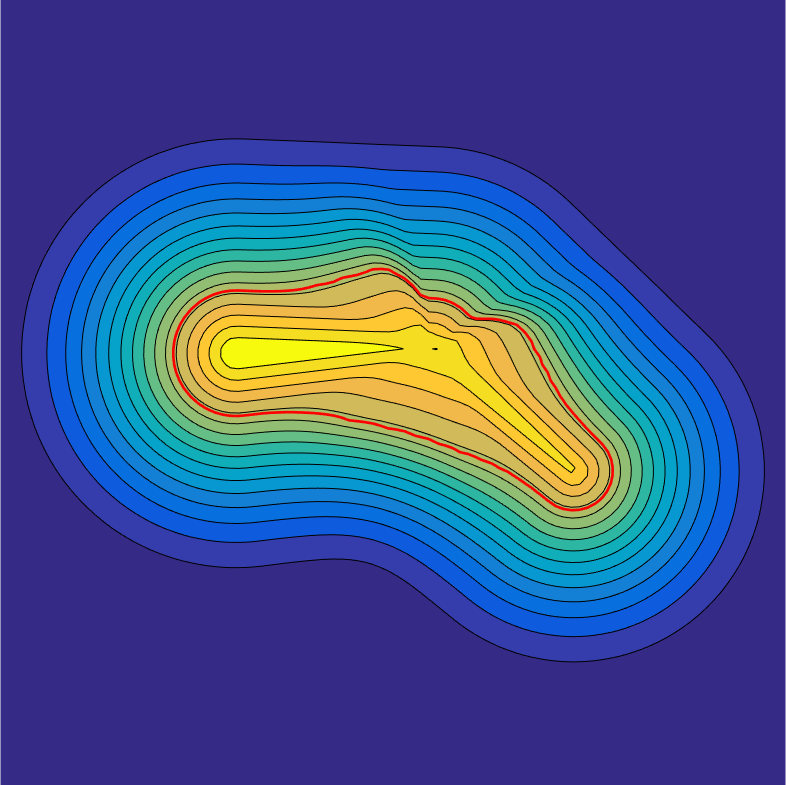
\includegraphics[width=0.22\textwidth]{figs/blend_finger_gradient}
\hfill
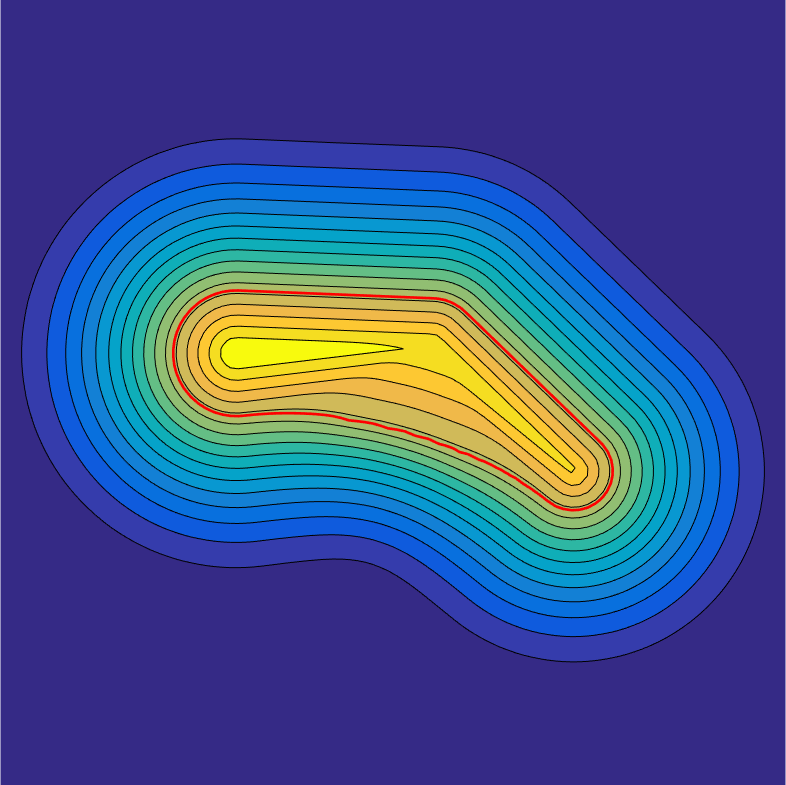
\includegraphics[width=0.22\textwidth]{figs/blend_finger_clamp}
\caption{Illustration of the blend strategies. On the left, the angle between gradients is used to blend the whole finger. On the right, the angle between bones is used to blend the lower part only.}
\end{figure}

The blend operator gradient could be analytically computed, but the performance cost is too high.
In practice, to reach high performances, gradients and signed distance function are discretized and precomputed.


\subsection{Surface tracking}
\label{section:surface_tracking}

\emph{Surface tracking} is used during animation to correct the mesh deformation produced either by linear blend or dual quaternion skinning \cite{Kavan:2008}.
The main idea is to project every vertex such that its isovalue is the same as it was in the rest pose.

In order to do this, two steps are repeated until convergence: \emph{vertex projection} and \emph{tangential relaxation}.
Finally, \emph{laplacian smoothing} is applied on contact regions to reduce sharp features.


\subsubsection{Vertex projection}

During the vertex projection step, each vertex $\mathbf{v}_i$ is moved along the gradient of the field function $f$, until it reaches its original isovalue $iso_i$.
We track the isovalues in the rest pose instead of the 0.5-isosurface to avoid losing the details of the mesh.
Newton iterations are used, with $\sigma = 0.35$, to provide a robust, fast and accurate convergence:

\begin{equation*}
\mathbf{v'}_i = \mathbf{v}_i + \sigma (iso_i - f(\mathbf{v}_i)) \frac{\nabla f(\mathbf{v}_i)}{\left\| \nabla f(\mathbf{v}_i) \right\| }
\end{equation*}

The main convergence criterion is when the vertex has reached its isovalue at rest:

\begin{equation*}
|iso_i - f(\mathbf{v}_i)| < \varepsilon
\end{equation*}

Additionally, in order to avoid generating self-intersections, we should stop iterating when vertices reach a contact region.
To detect this case, Vaillant proposes the following test.

For every vertex, we know the gradient at the current iteration and at the previous one.
If the angle between these two vectors is greater than $55°$, we consider that the vertex lies on a contact surface.
The idea is that the gradient will flip when a vertex crosses from one implicit surface to another.


\subsubsection{Tangential relaxation}

This step is used to improve the distribution of the vertices.
High distortions can be introduced by the vertex projection.
Vertices are therefore moved toward the weighted centroid of their neighbours.
Barycentric coordinates $\Phi_{ij}$ are precomputed in the rest pose for each vertex $\mathbf{v}_i$ with respect to its one-ring neighbours.
After each vertex projection, the tangential relaxation relocates vertices to avoid drift:

\begin{equation*}
\mathbf{v}_i' = (1 - \mu) \mathbf{v}_i + \mu \sum_j \Phi_{ij} \mathbf{q}_{ij},
\end{equation*}

where $\mathbf{q}_{ij}$ are the one-ring neighbours of $\mathbf{v}_i$ projected onto its the tangential plane and the coefficient $\mu$ is used to control the strength of the operation.
It is defined as a function of the distance to the isovalue in the rest pose, so that it decreases as the vertex approaches convergence:

\begin{equation*}
\mu = \max\left(0, 1 - \left(|iso_i - f(\mathbf{v}_i)| - 1\right)^4\right)
\end{equation*}

Since computing generalized barycentric coordinates is not trivial, we give a summary of the method we used for this: the \emph{mean value coordinates} \cite{Hormann:2006}.
Given a vertex $\mathbf{v}$, the goal is to find weights $\Phi_j$ such that $\mathbf{v} = \sum_j \Phi_j \mathbf{q}_j$, with $\mathbf{q}_j$ the one-ring neighbours projected onto the tangential plane of $\mathbf{v}$.

First, let's assume we can traverse the neighbours cyclically.
We compute the weight of each neighbour $j$ as:

\begin{equation*}
\Phi_j = \frac{\tan(\alpha_{j-1} / 2) + \tan(\alpha_j / 2)}{r_j}
\end{equation*}

The weights are then normalized such that $\sum_j \Phi_j = 1$.
The notations used are described in figure \ref{fig:mvc}.

For the case where the vertex $\mathbf{v}$ is on a mesh boundary, we cannot cycle through the neighbours.
To deal with this issue, we do not apply the tangential relaxation on the vertices that are on a mesh boundary.

\begin{figure}[H]
\centering
\begin{tikzpicture}
\coordinate [label = {above:$\mathbf{v}$}] (v) at (0,0); 
\coordinate (q1) at (-2,-1.5);
\coordinate (q2) at (3.8,-1.3);
\coordinate (q3) at (3,0.3);
\coordinate (q4) at (-1.4,0.7);
\coordinate (q5) at (-3,0.2);
\draw (q1) -- (q2) -- (q3) -- (q4) -- (q5) -- (q1); % Neighbours path
\draw (v) -- (q1) node[below] {$\mathbf{q}_{j-1}$}; % v_i to q1
\draw (v) -- node[midway, below left] {$r_j$} (q2) node[below right] {$\mathbf{q}_{j}$}; % v_i to q2
\draw (v) -- (q3) node[above right] {$\mathbf{q}_{j+1}$}; % v_i to q3
\foreach \i in {4,...,5}{\draw (v) -- (q\i);}
\draw[->] (-0.8, -0.6) to[bend right=20] node[midway, below] {$\alpha_{j-1}$} (0.9462, -0.3237);
\draw[->] (1.4192, -0.4855) to[bend right=50] node[midway, right] {$\alpha_j$} (1.4926, 0.1493);
\end{tikzpicture}
\caption{Notations used for the mean value coordinates.}
\label{fig:mvc}
\end{figure}


\subsubsection{Laplacian smoothing}

Finally, laplacian smoothing is used to remove sharp features introduced by the self-intersection heuristic.
This step must be applied immediately after the last vertex projection:
\begin{equation*}
\mathbf{v}_i = (1 - \beta_i) \mathbf{v}_i + \beta_i \tilde{\mathbf{v}}_i
\end{equation*}
Each vertex $\mathbf{v}_i$ is moved toward the centroid $\tilde{\mathbf{v}}_i$ of its one-ring neighborhood.
The smoothing coefficient $\beta_i$ is set to $1$ for vertices stopped at a gradient discontinuity, $0$ for the others.
To have a clean transition, the values $\beta_i$ are interpolated using diffusion prior to applying the smoothing.

\begin{figure}[H]
\centering
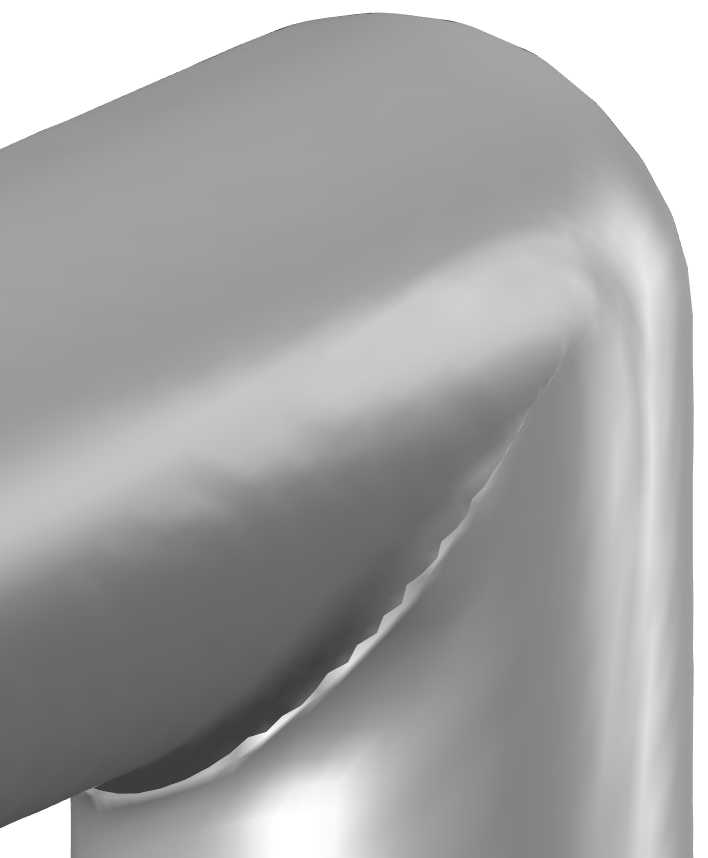
\includegraphics[width=0.20\textwidth]{figs/cylinder_no_laplacian}
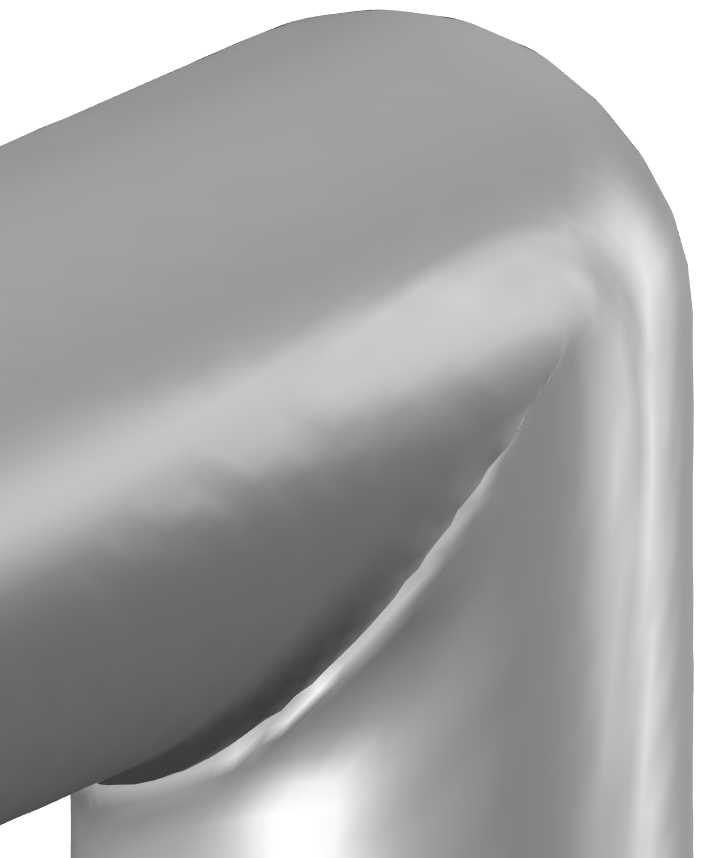
\includegraphics[width=0.20\textwidth]{figs/cylinder_laplacian}
\caption{Without smoothing (left), the mesh surface exhibits a sawtooth pattern.
Laplacian smoothing removes these oscillations.}
\end{figure}


\subsection{Hand registration}
\label{section:registration}

Since this project is associated to hand tracking, some issues unrelated to implicit skinning might arise.
Sphere positions are used as input of our implementation.
These control points are located using computer vision and constrained through model-based registration.
Unfortunately, these locations depends on the morphology of the user hand.
Incoherent bone lengths is fixed by our pose estimator, in order to match the mesh metrics, which leads to an inaccurate representation.
Therefore the hand model should correspond to the user skeleton.

The obvious choice is to regenerate required data for any new user.
Many tools provide 3D reconstruction based on pictures, which can be used to generate a point cloud.
Usually noisy, this model can then be refined to obtain satisfactory results.
More time-consuming techniques can also be applied, like designing the mesh by hand, using modeling tools.
But for non-professional purpose, several hours of work by a designer may be inappropriate.

Moreover, some details must be adjusted to fit the new model.
The majority of the pipeline does not depends on the actual mesh, as long as the topology is preserved.
However, bone locations and vertex weights need to be defined.
As this was proven during this project, this is a tedious and non-trivial task.

To solve this issue, we have tried to apply rigid registration, as successfully applied to human faces by Bouaziz\cite{Bouaziz:2013:DRK:2504435.2504456}.
By automatically generating a mapping between our neutral mesh and the user scan, data could be acquired in a cheaper way.
Sphere locations and weights could be exported to the new mesh.
Furthermore, the clean neutral mesh could be used instead of the noisy and ill-triangulated point cloud.

\begin{figure}[H]
\centering
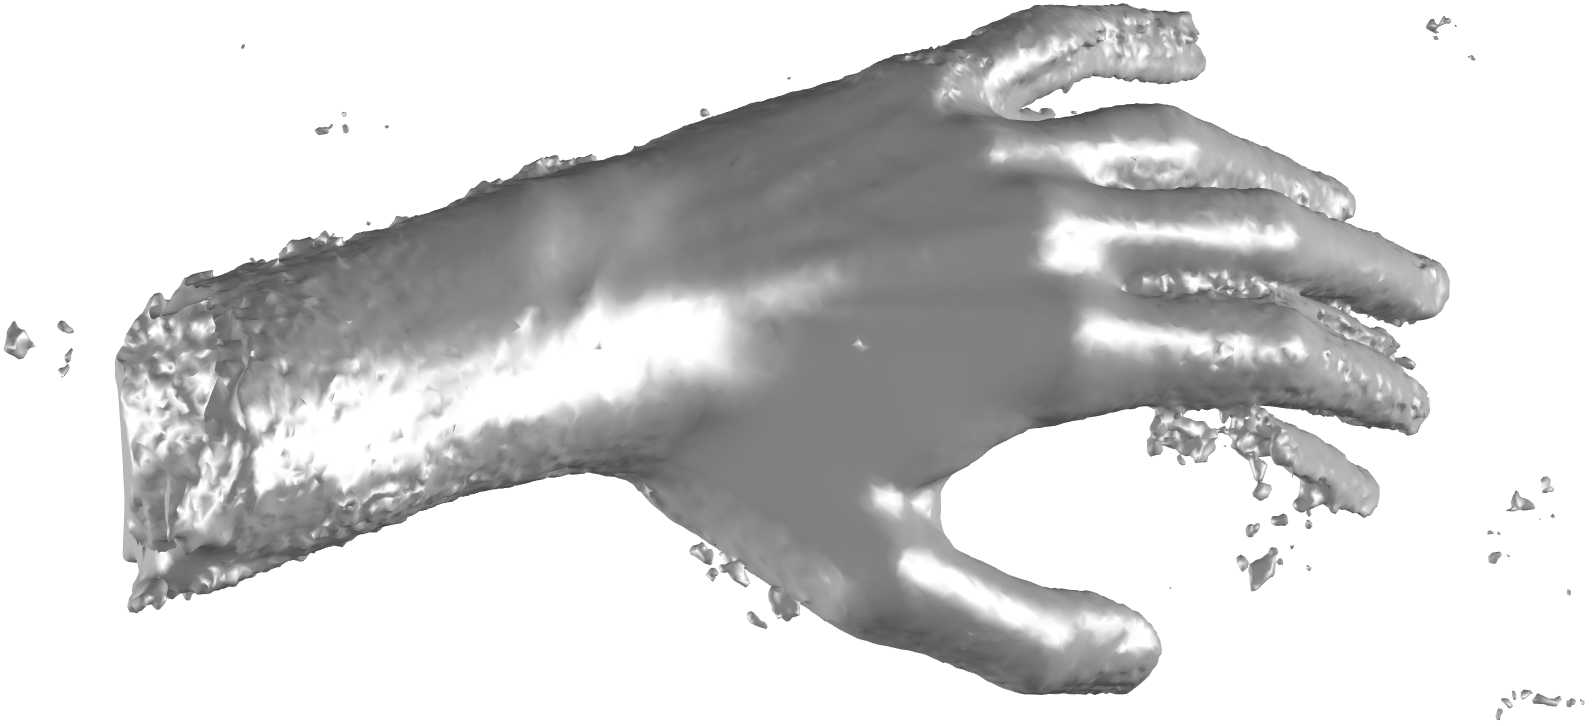
\includegraphics[width=0.45\textwidth]{figs/registration_cloud}
\caption{A point cloud generated from several pictures.
Cleaning this mesh and adjusting bone locations is not a trivial task.}
\end{figure}

As the hand has many more degrees of freedom than the face, some changes must be applied to the original algorithm.
The main difficulty is to estimate the point cloud pose.
We have tried several optimization strategies, without significant success.
The most promising approach was highly specialized feature detection.
By first locating the palm, the global size of the hand can be estimated.
Then, each phalange is fit sequentially, until the global pose is acquired.

Since this issue was not the top priority of this work, hand registration was too time-consuming to be completed.
Good approximations were reached, but without sufficient precision to be a viable alternative to manual design.

\begin{figure}[H]
\centering
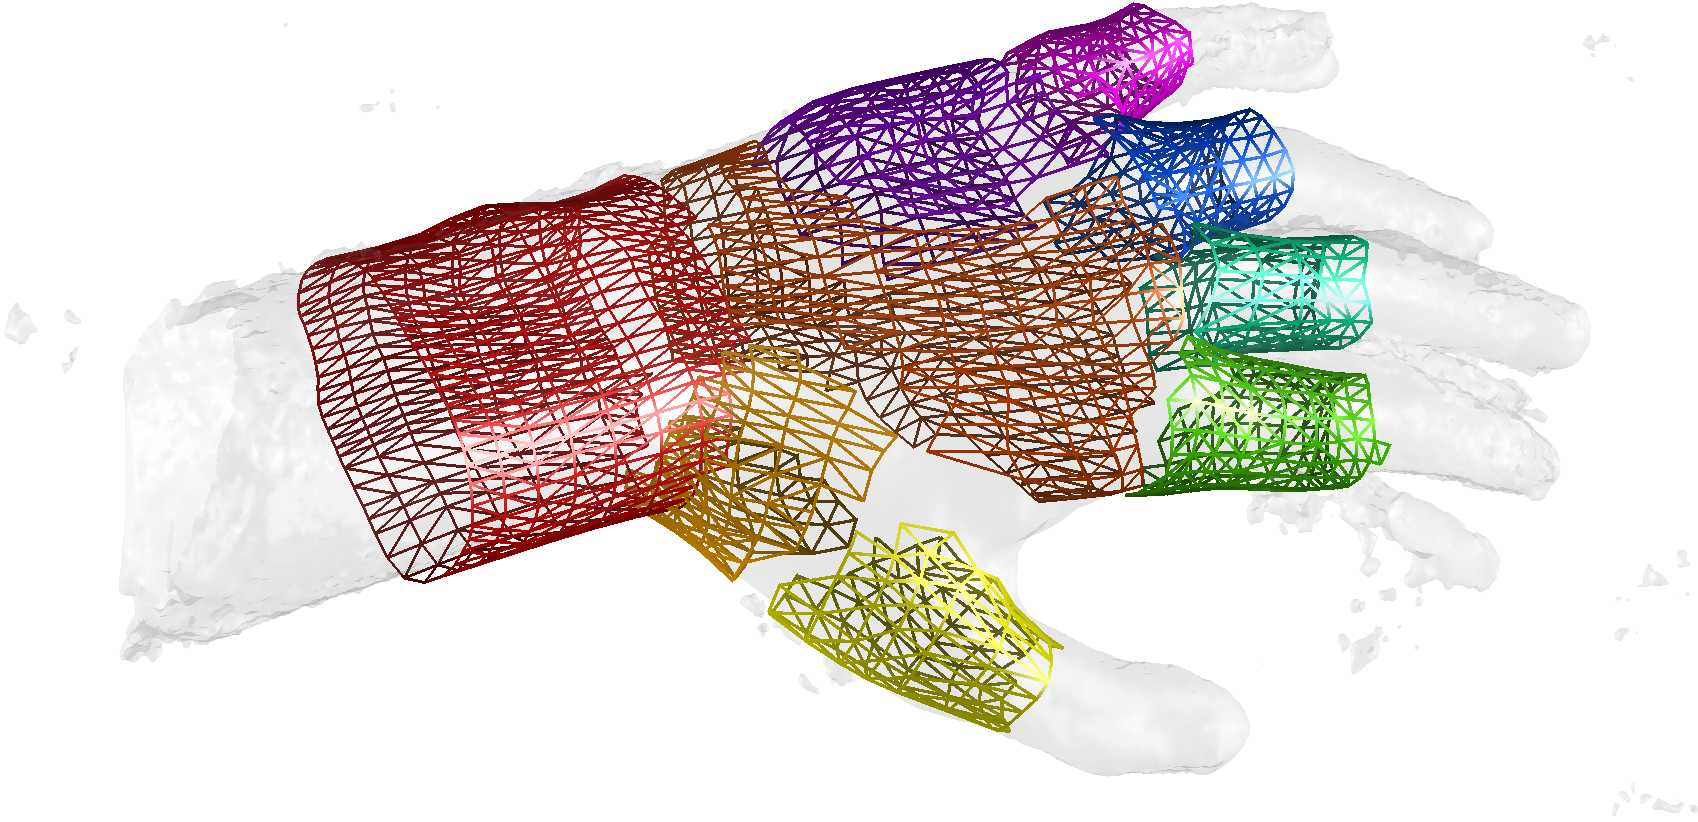
\includegraphics[width=0.45\textwidth]{figs/registration_attempt}
\caption{Palm, wrist and some phalanges were fit using the Iterative Closest Point algorithm.
Better alternatives could be used, as the Sparse ICP by Bouaziz \cite{Bouaziz:2013:SIC:2600289.2600305}.}
\end{figure}


\section{Implementation and results}
\label{section:results}

We were given as inputs a mesh of a hand and the positions of the spheres.
As explained in the theory, the first part was to define a bone hierarchy and create skinning weights.
The placement of the bones was based on the positions of the spheres.

\begin{figure}[H]
\centering
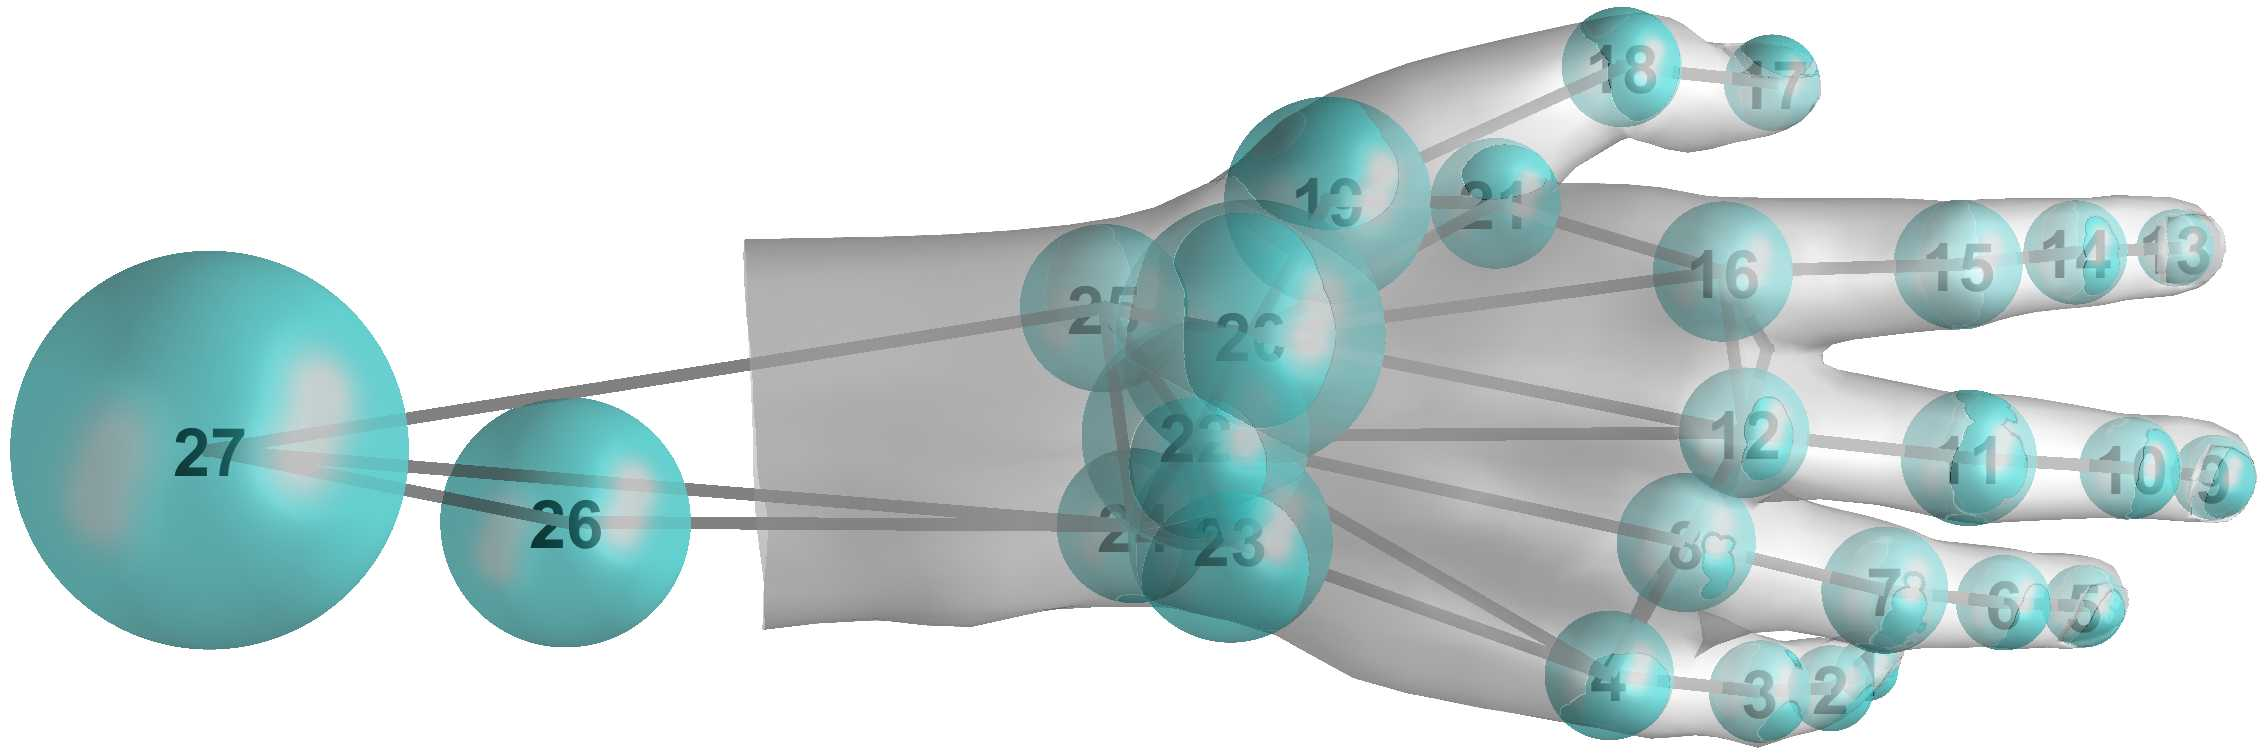
\includegraphics[width=0.45\textwidth]{figs/hand_spheres}
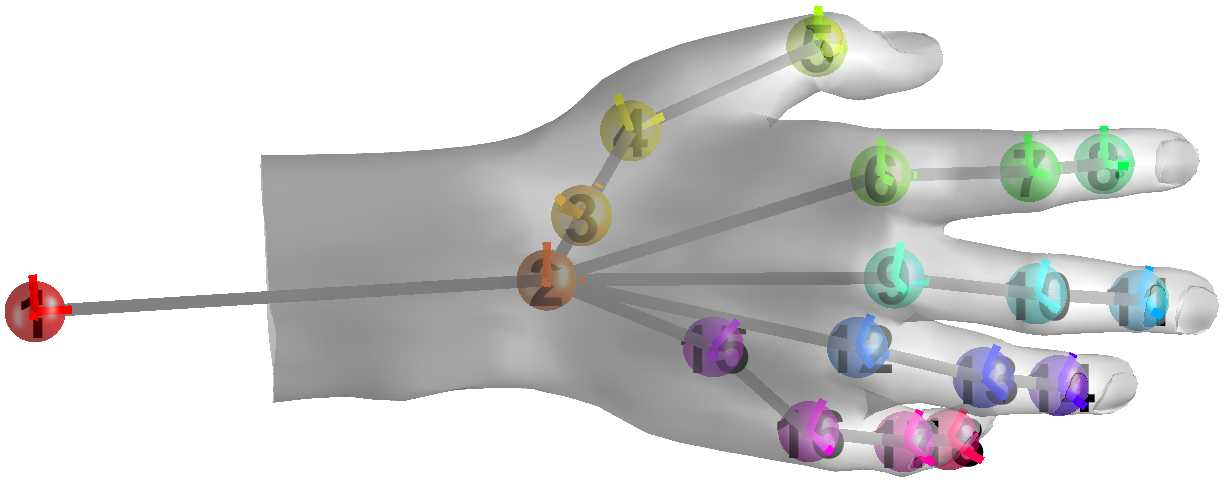
\includegraphics[width=0.40\textwidth]{figs/hand_bones}
\caption{The hand mesh and the spheres that are provided as inputs (top).
The hierarchy of bones (bottom) is based on the positions of the spheres.}
\end{figure}

Blender was used to create and tweak the skinning weights.
Based on the weights, we were able to partition the mesh around every bone.
More precisely, every vertex was assigned to the bone with the highest weight.
The following figure illustrates this process.

\begin{figure}[H]
\centering
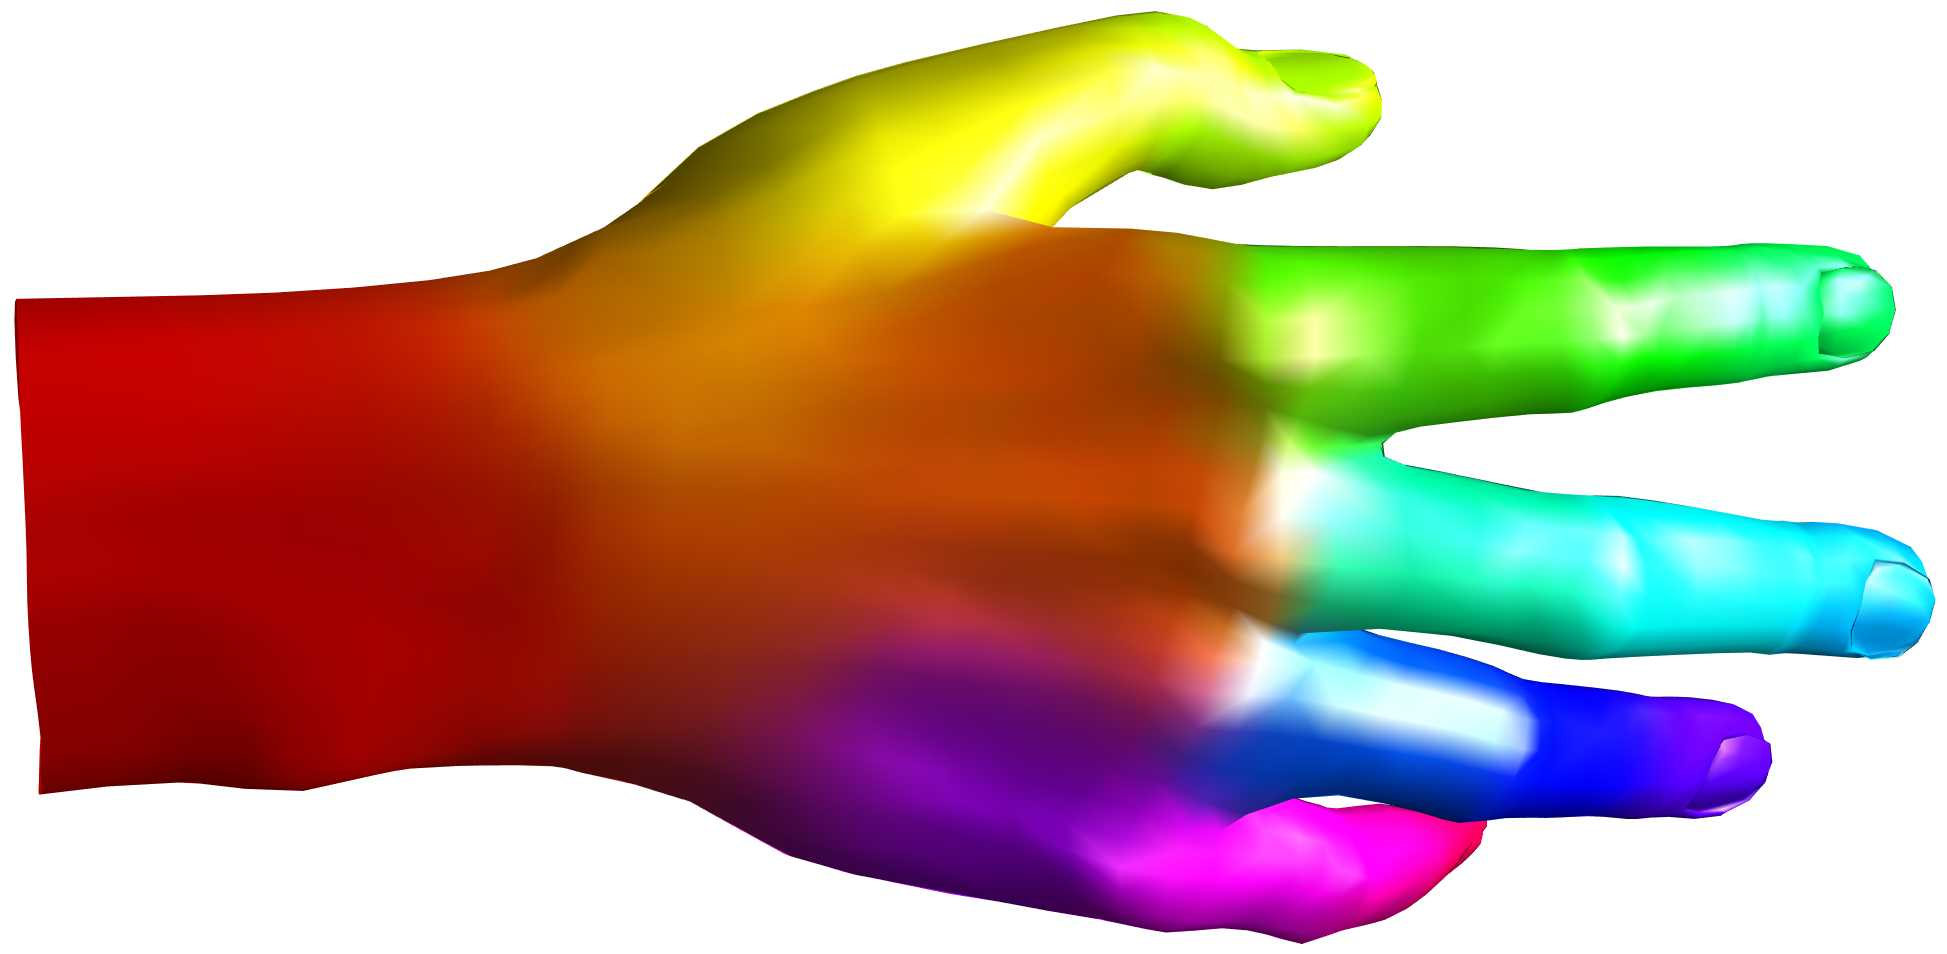
\includegraphics[width=0.45\textwidth]{figs/hand_bone_weights}
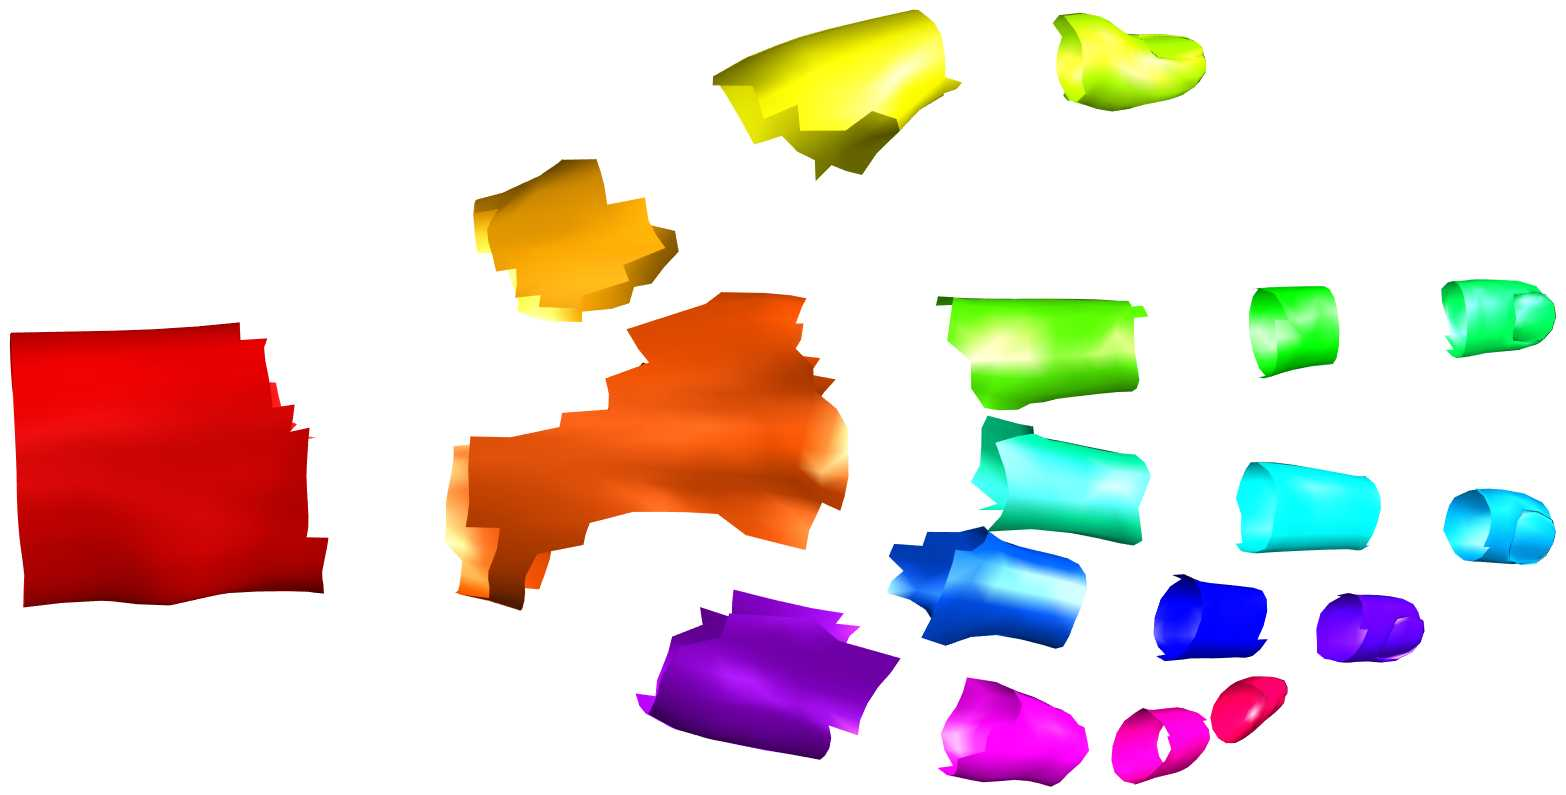
\includegraphics[width=0.45\textwidth]{figs/hand_bone_partition}
\caption{The hand mesh and its partitioning.
Each color corresponds to the area of influence of a bone.}
\end{figure}

This partitioning is needed for the surface reconstruction, which was done with HRBFs and spherical primitives.
In the case of the latter, the positions of the spheres are given as inputs and each sphere is assigned to a bone, so there was little work to do to reconstruct the surface.

Getting correct approximations of the mesh surface with HRBFs was a bit more challenging.
The first problem we solved was to fill the holes left at the extremities of the partitions.
This is important because two neighbouring surfaces should joint without introducing gaps or gradient discontinuities.

Another problem was the choice of the HRBF's centers and control points.
Poisson disk sampling on the mesh proved to be a good strategy, because it avoids having multiple samples too tightly packed.
Even with this, it may happen that the reconstruction of a part does not smoothly follow the mesh surface.
To tackle this problem, we wrote a Matlab script where a reconstruction is showed and the user can accept or reject it, in which case, we resample the mesh.
This allows to tweak the surfaces, if needed.

\begin{figure}[H]
\centering
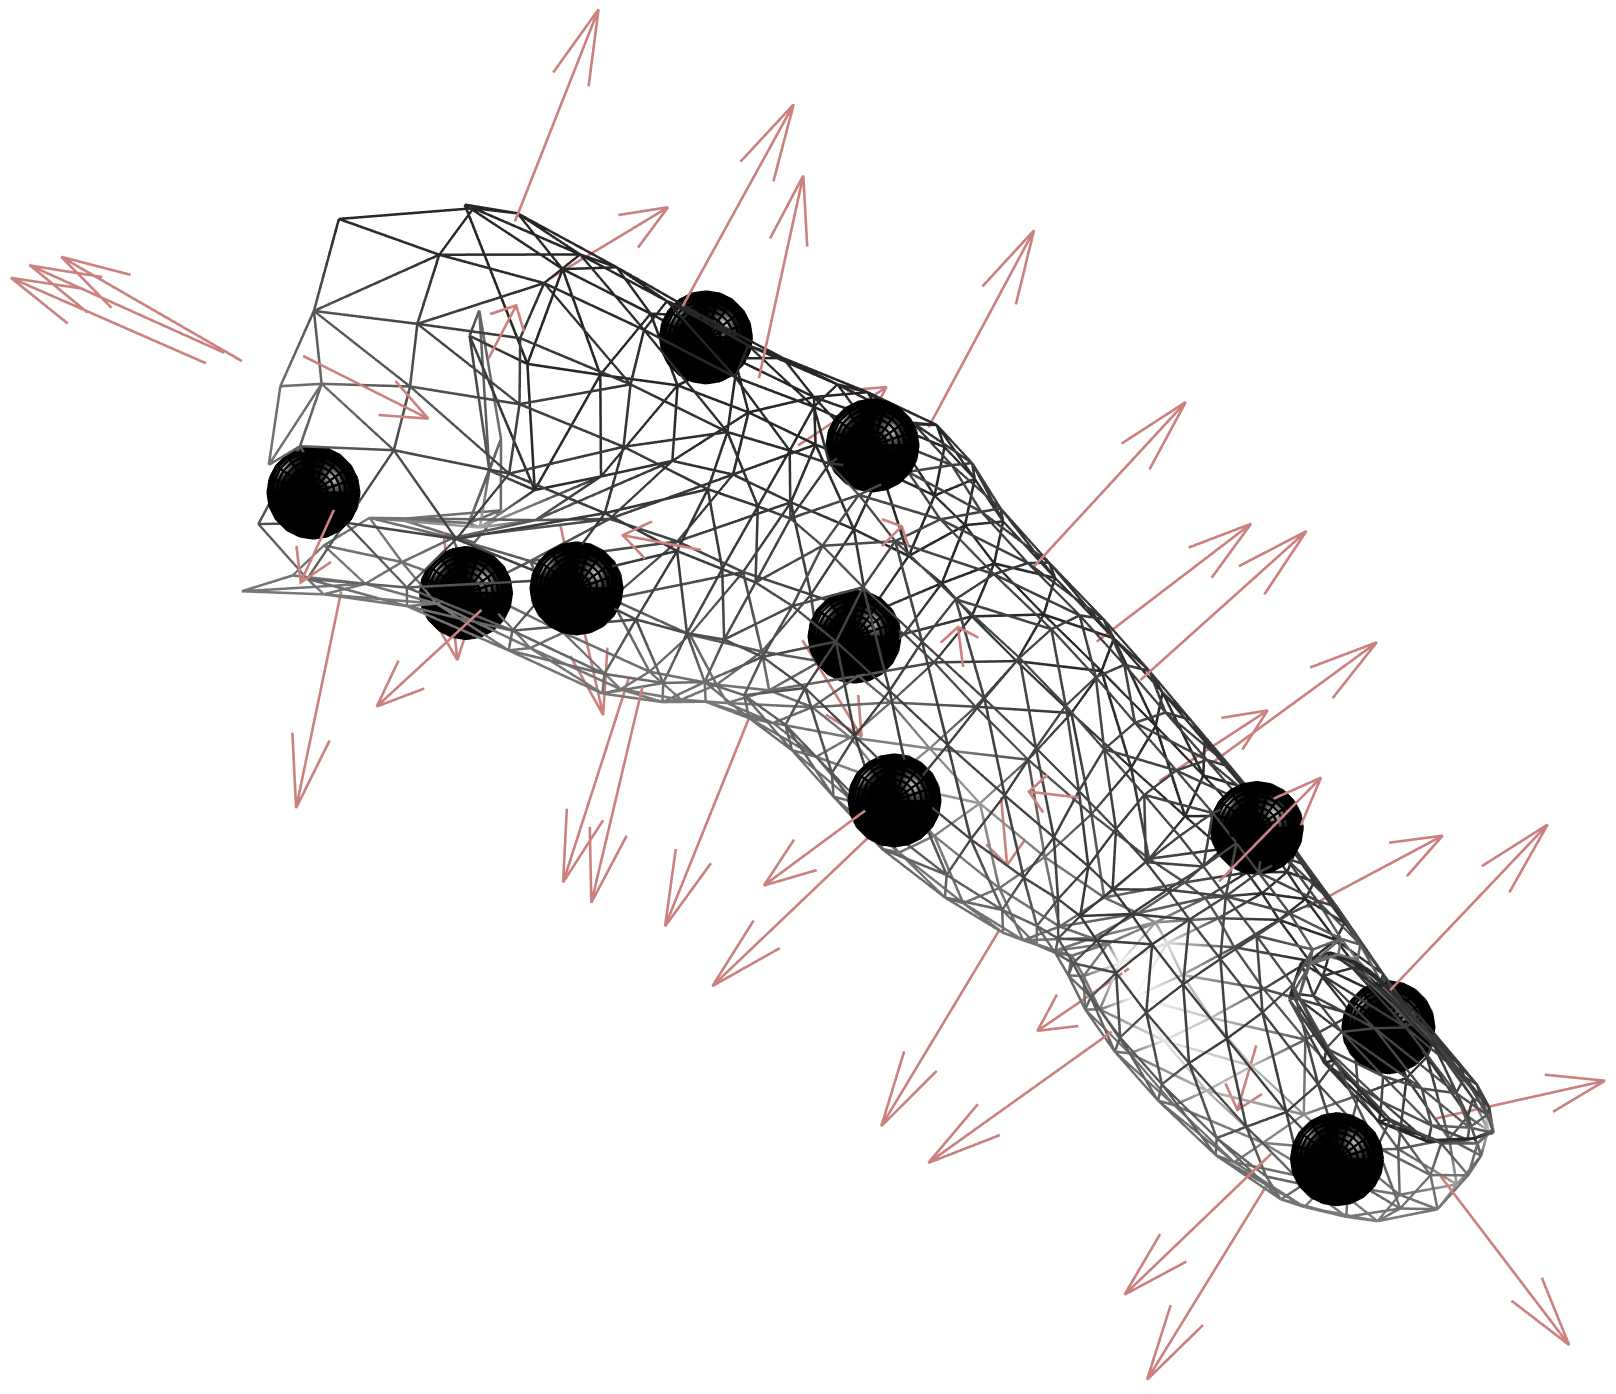
\includegraphics[width=0.23\textwidth]{figs/hrbf_centers}
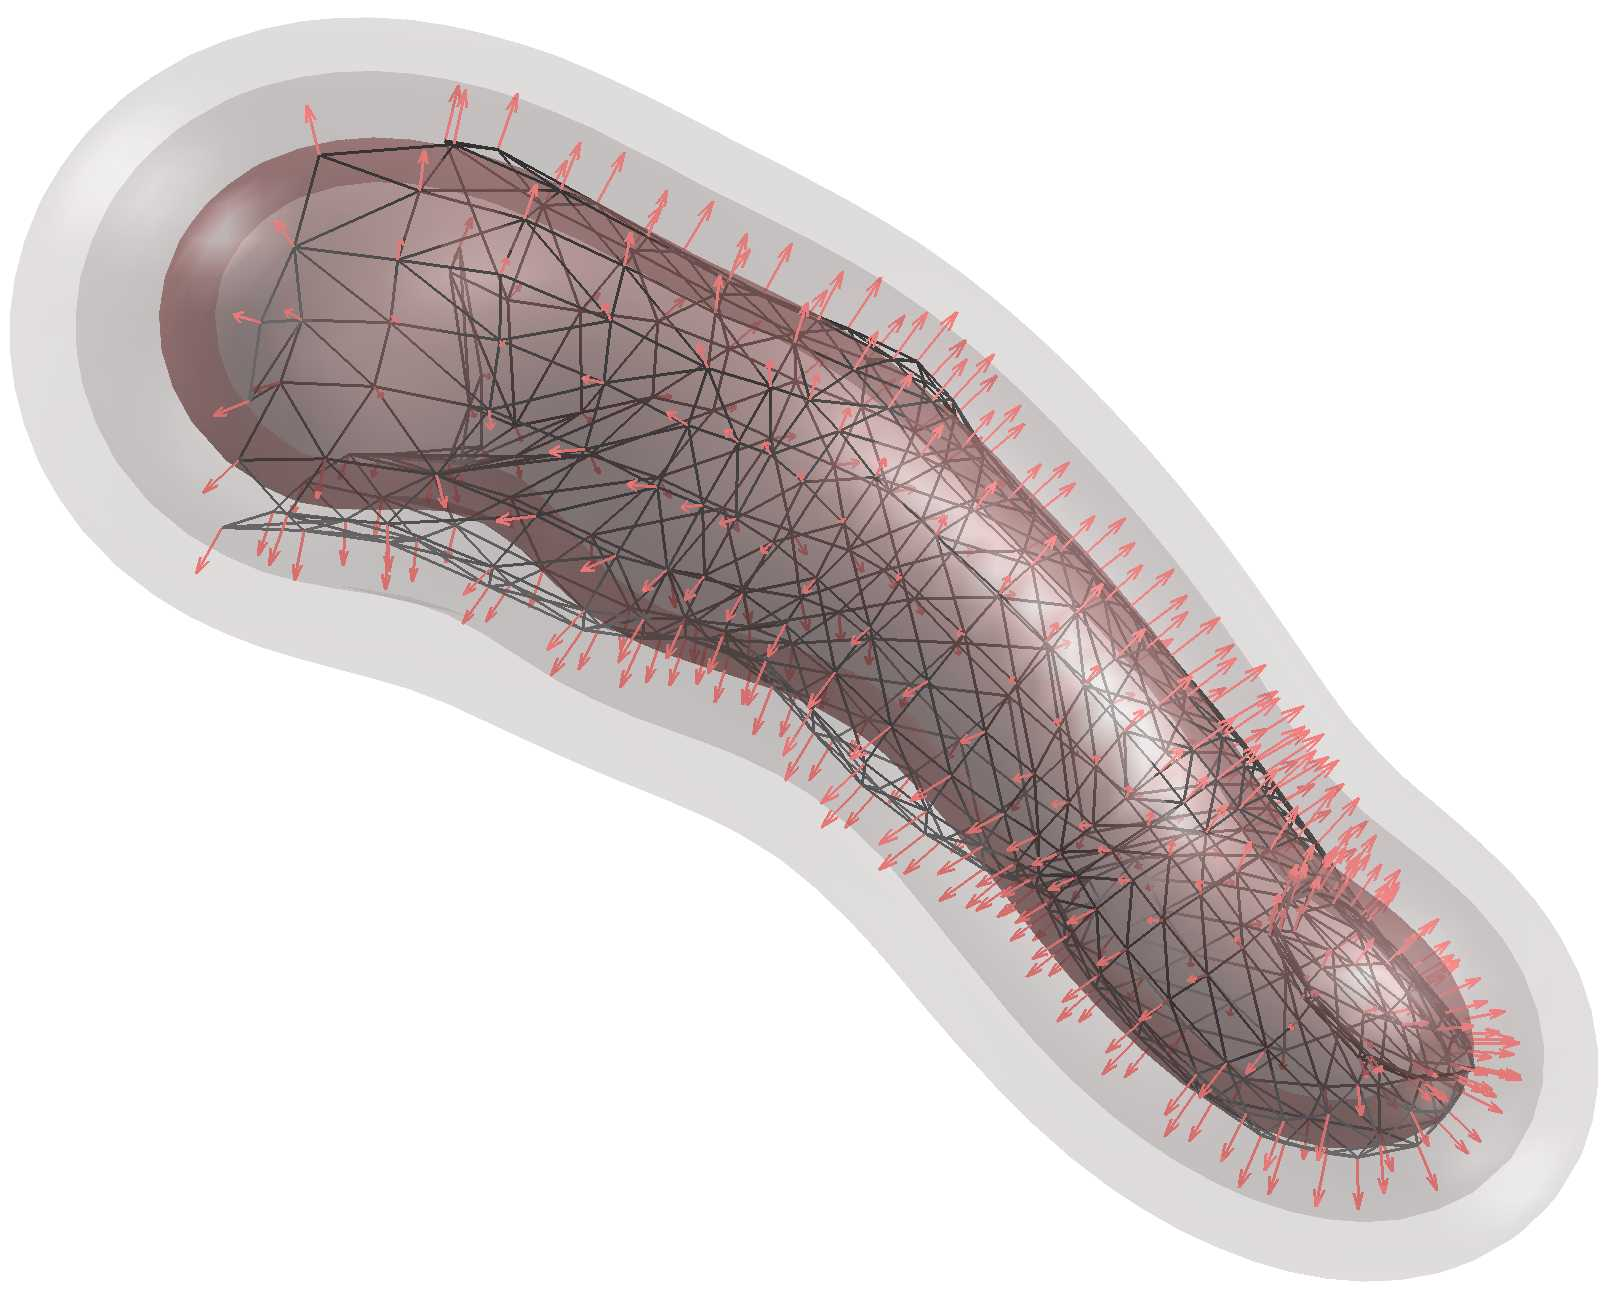
\includegraphics[width=0.23\textwidth]{figs/hrbf_reconstruction}
\caption{Illustration on a finger of the HRBF sampling (left) and the surface reconstruction (right).
The spheres represent the HRBF centers while the arrows are the positions and normal vectors used as control points.}
\end{figure}

\begin{figure}[H]
\centering
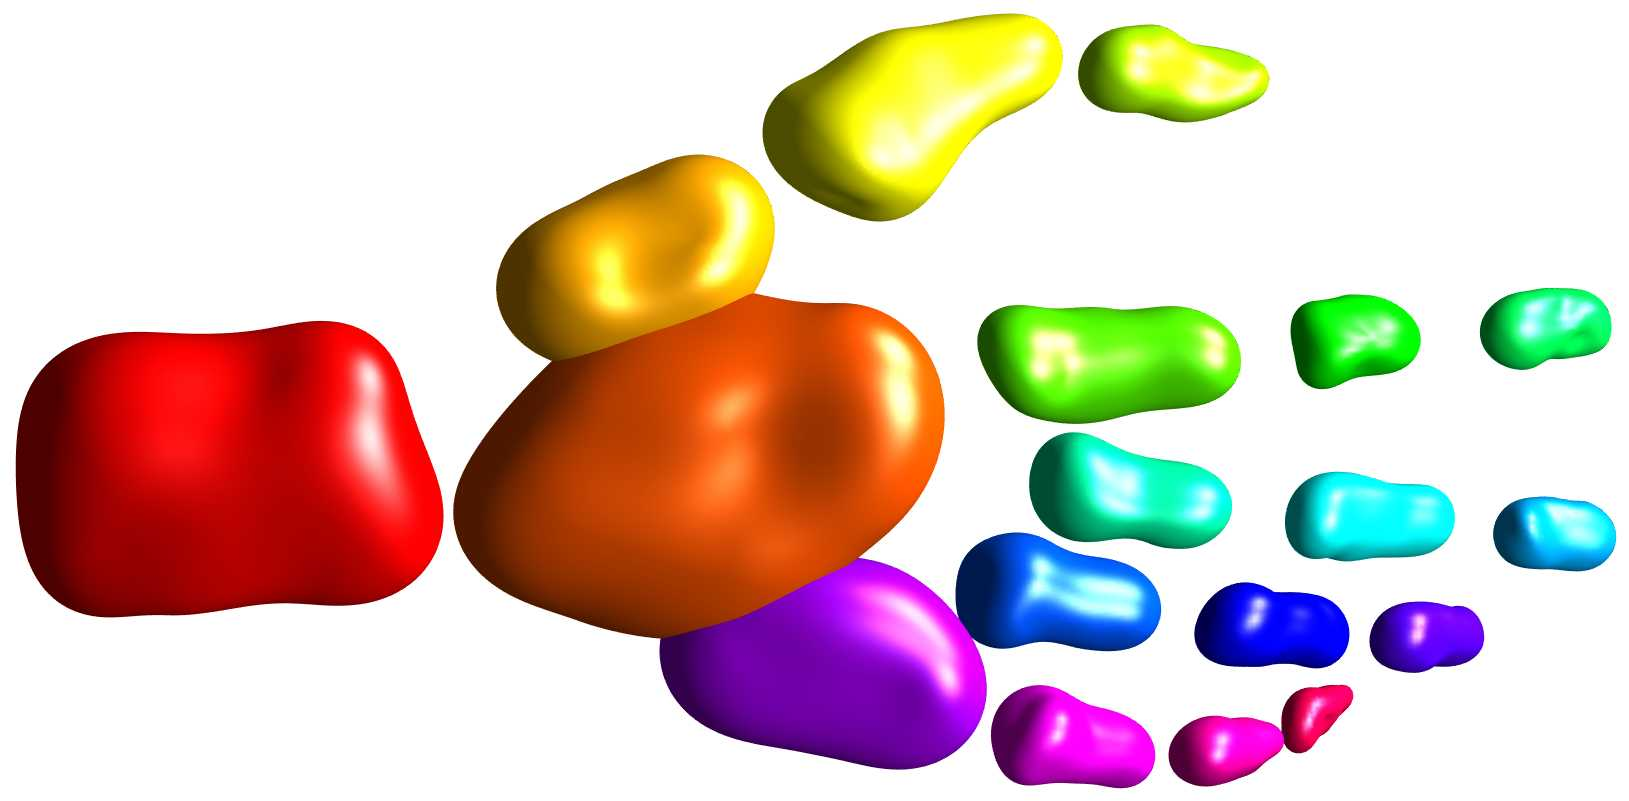
\includegraphics[width=0.45\textwidth]{figs/hand_bone_hrbf}
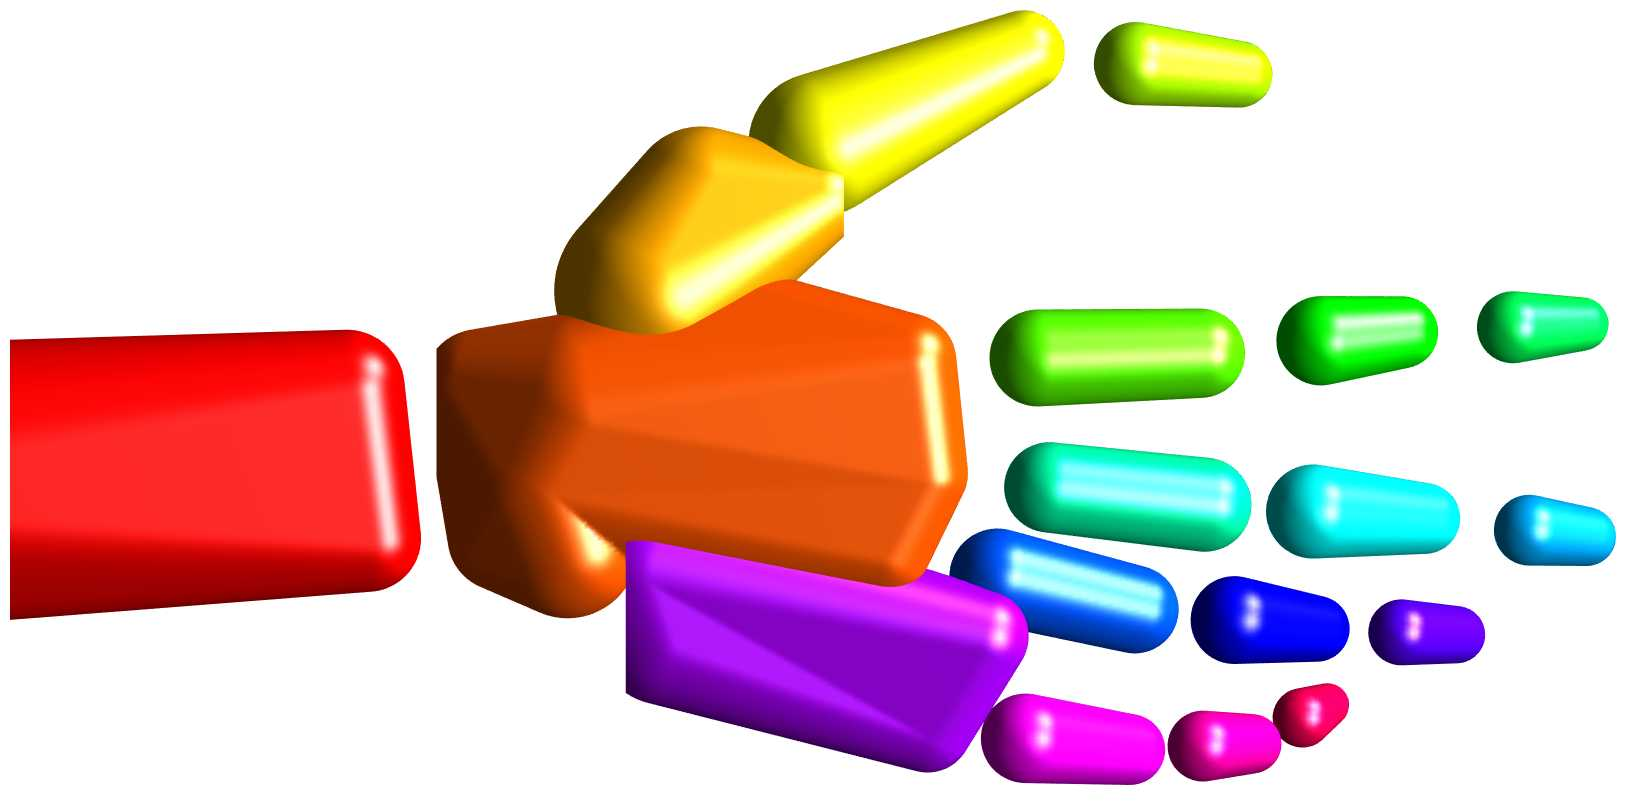
\includegraphics[width=0.45\textwidth]{figs/hand_bone_sphere}
\caption{Reconstruction of the mesh surface using HRBFs (top) and spherical primitives (bottom).}
\end{figure}

As we explained, surfaces should slide over each others at joints, in order to avoid gaps.
From that regard, the spherical primitives are better, as we can see in the following figure.

\begin{figure}[H]
\centering
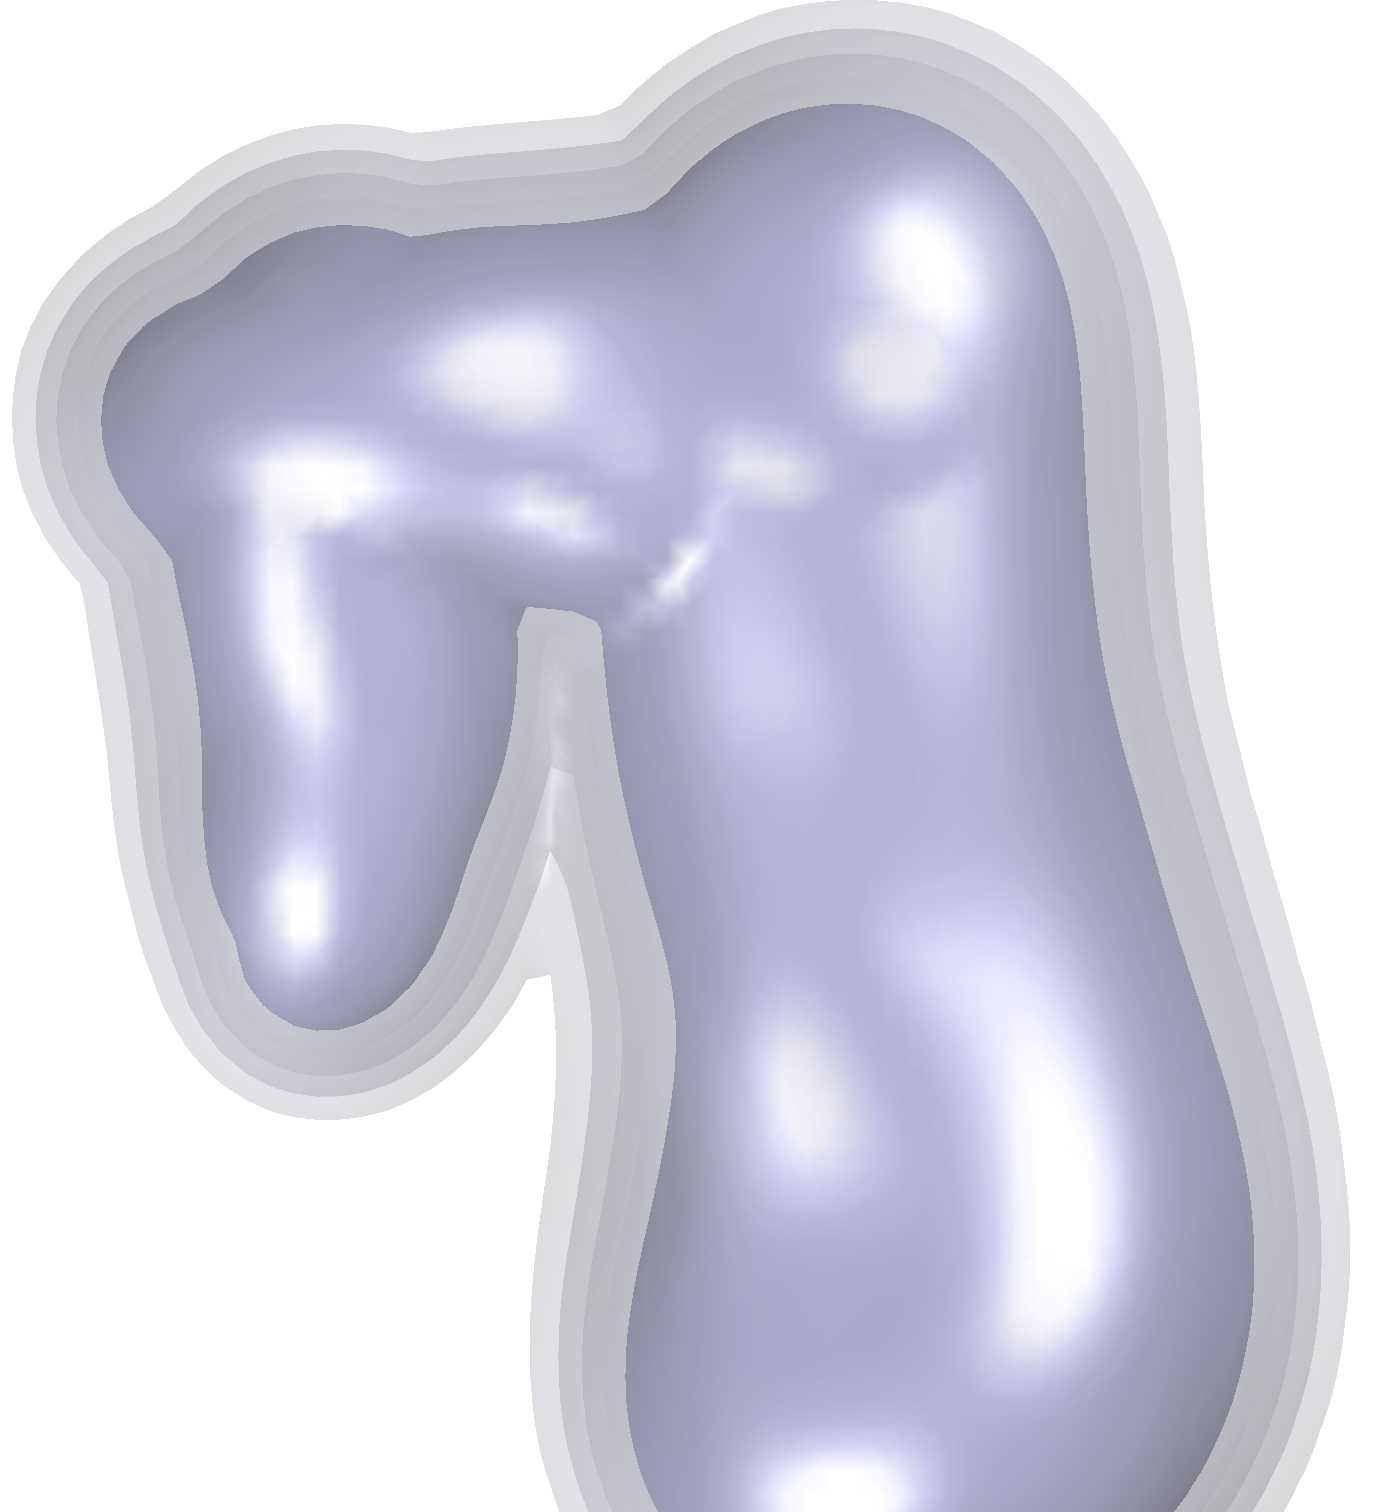
\includegraphics[width=0.14\textwidth]{figs/index_sdf_hrbf_union_bad}
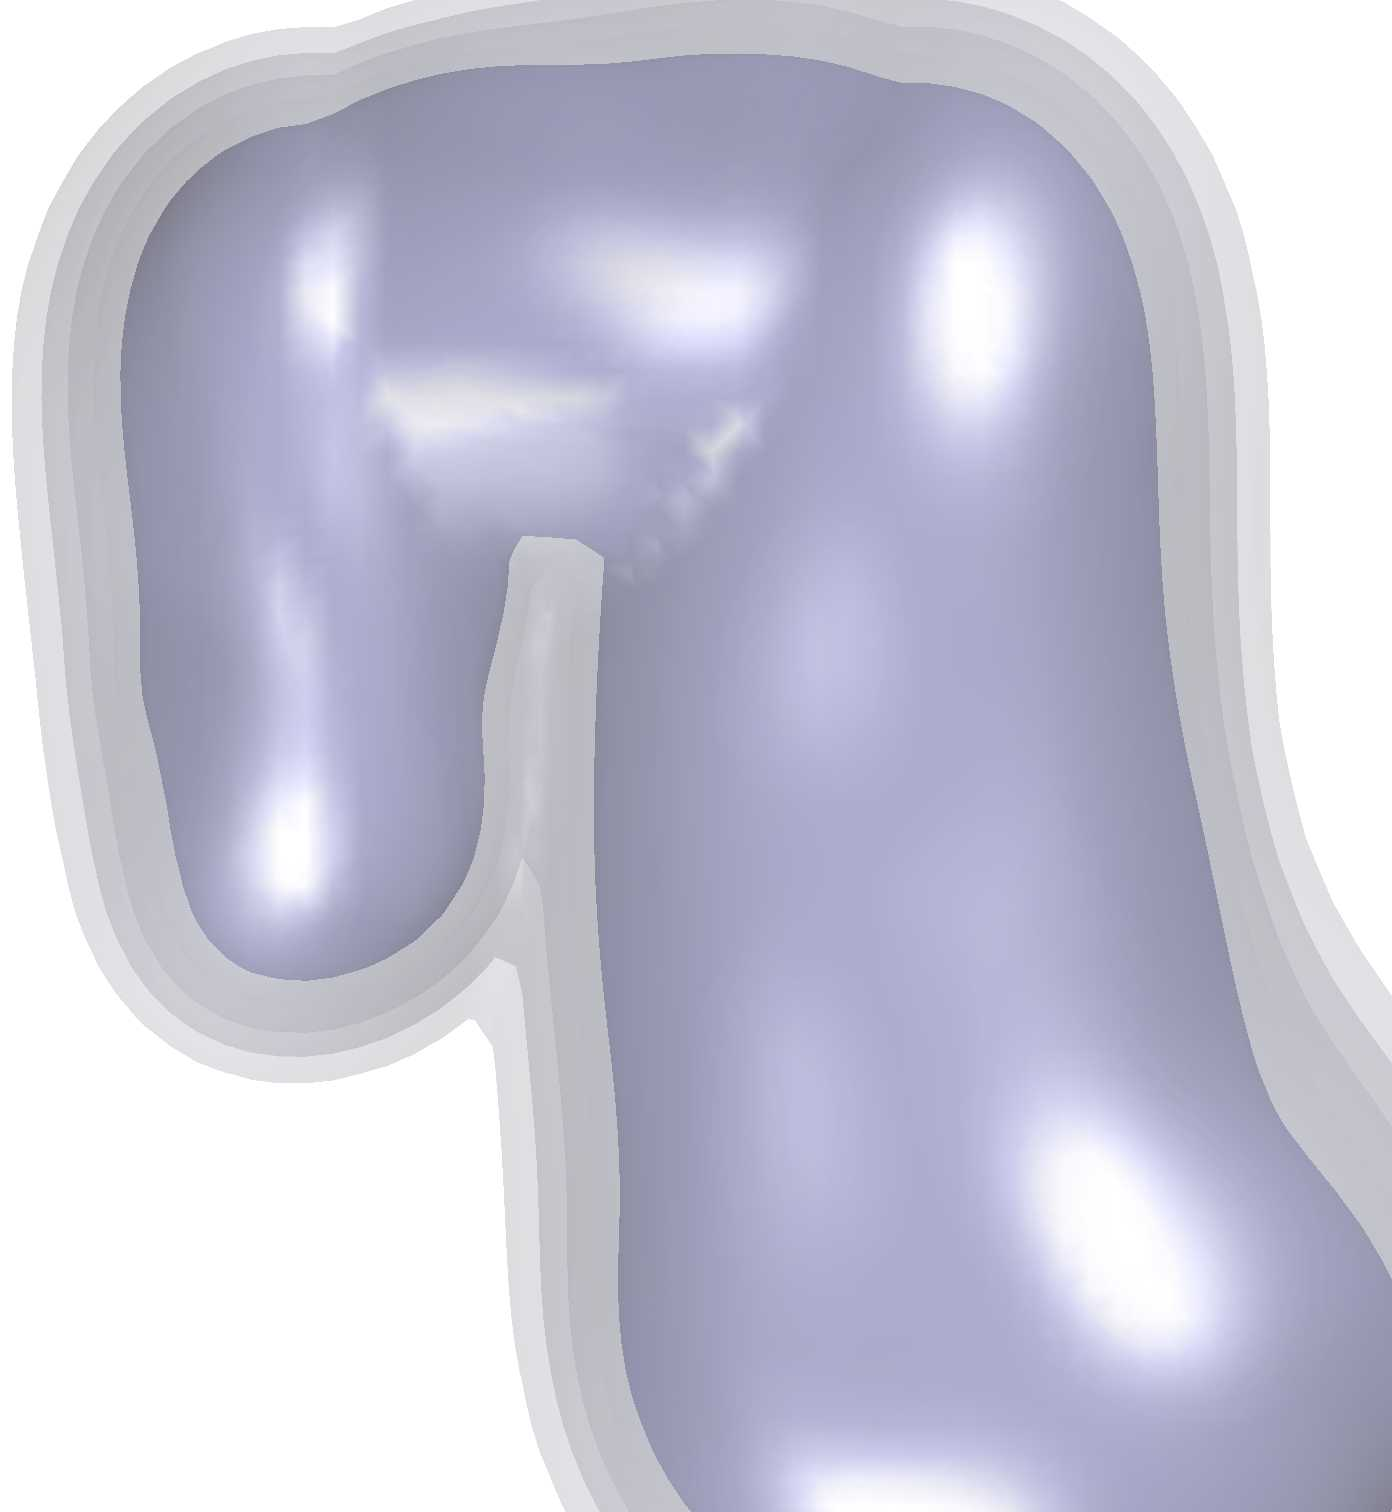
\includegraphics[width=0.14\textwidth]{figs/index_sdf_hrbf_union}
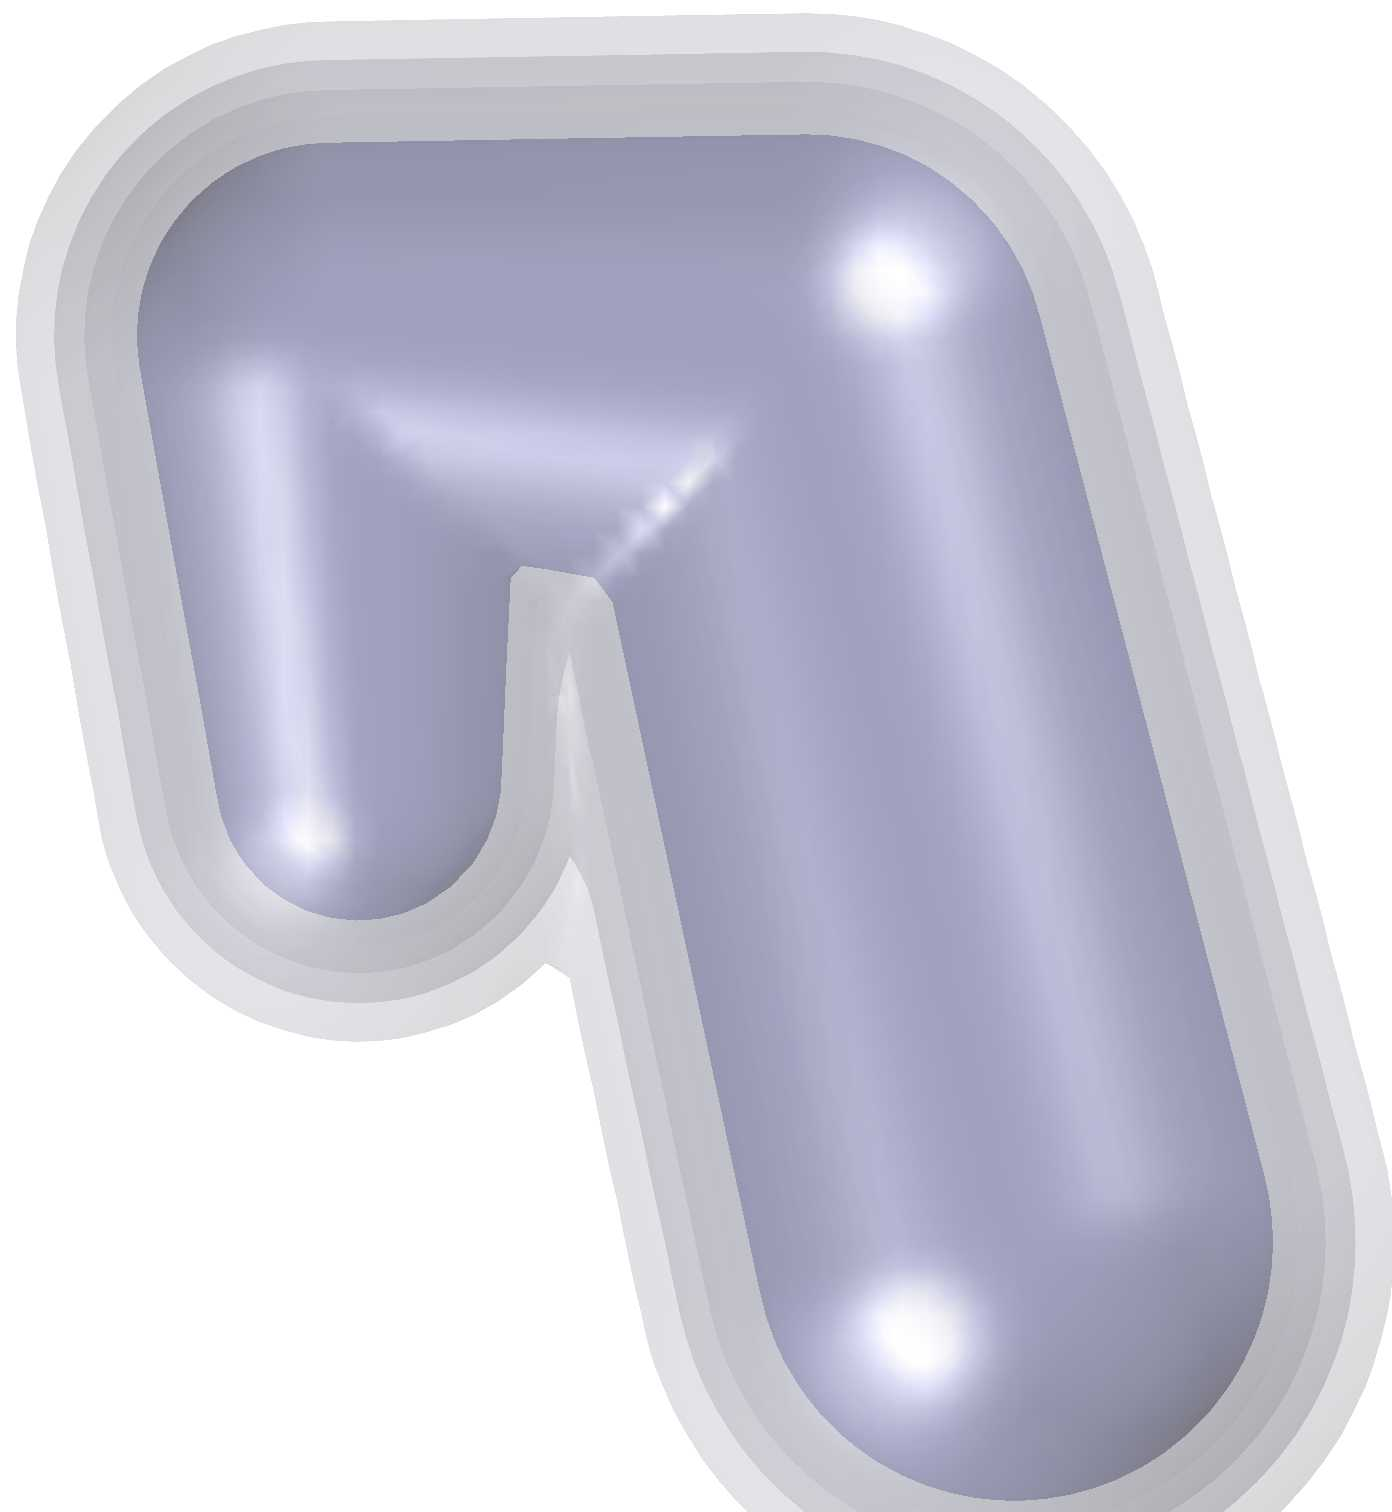
\includegraphics[width=0.14\textwidth]{figs/index_sdf_sphere_union} \\
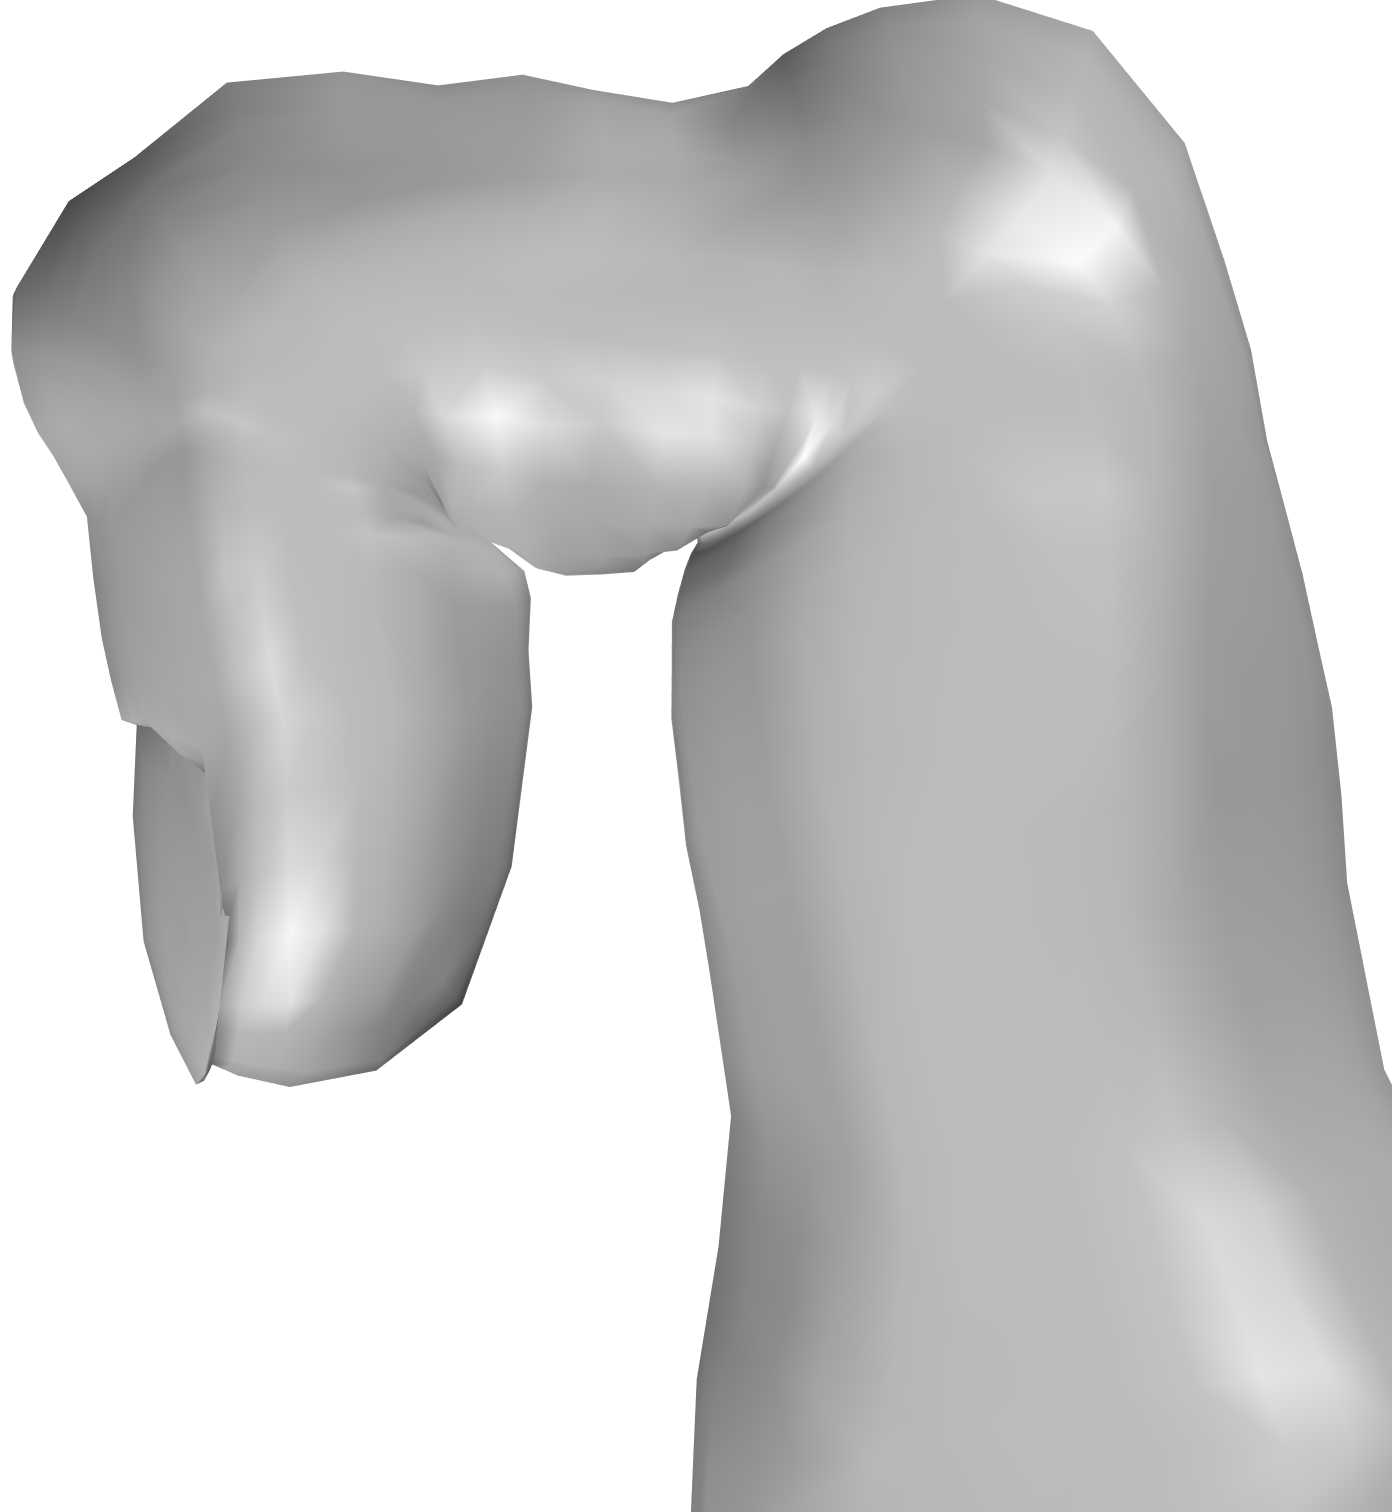
\includegraphics[width=0.14\textwidth]{figs/index_implicit_bad_hrbf}
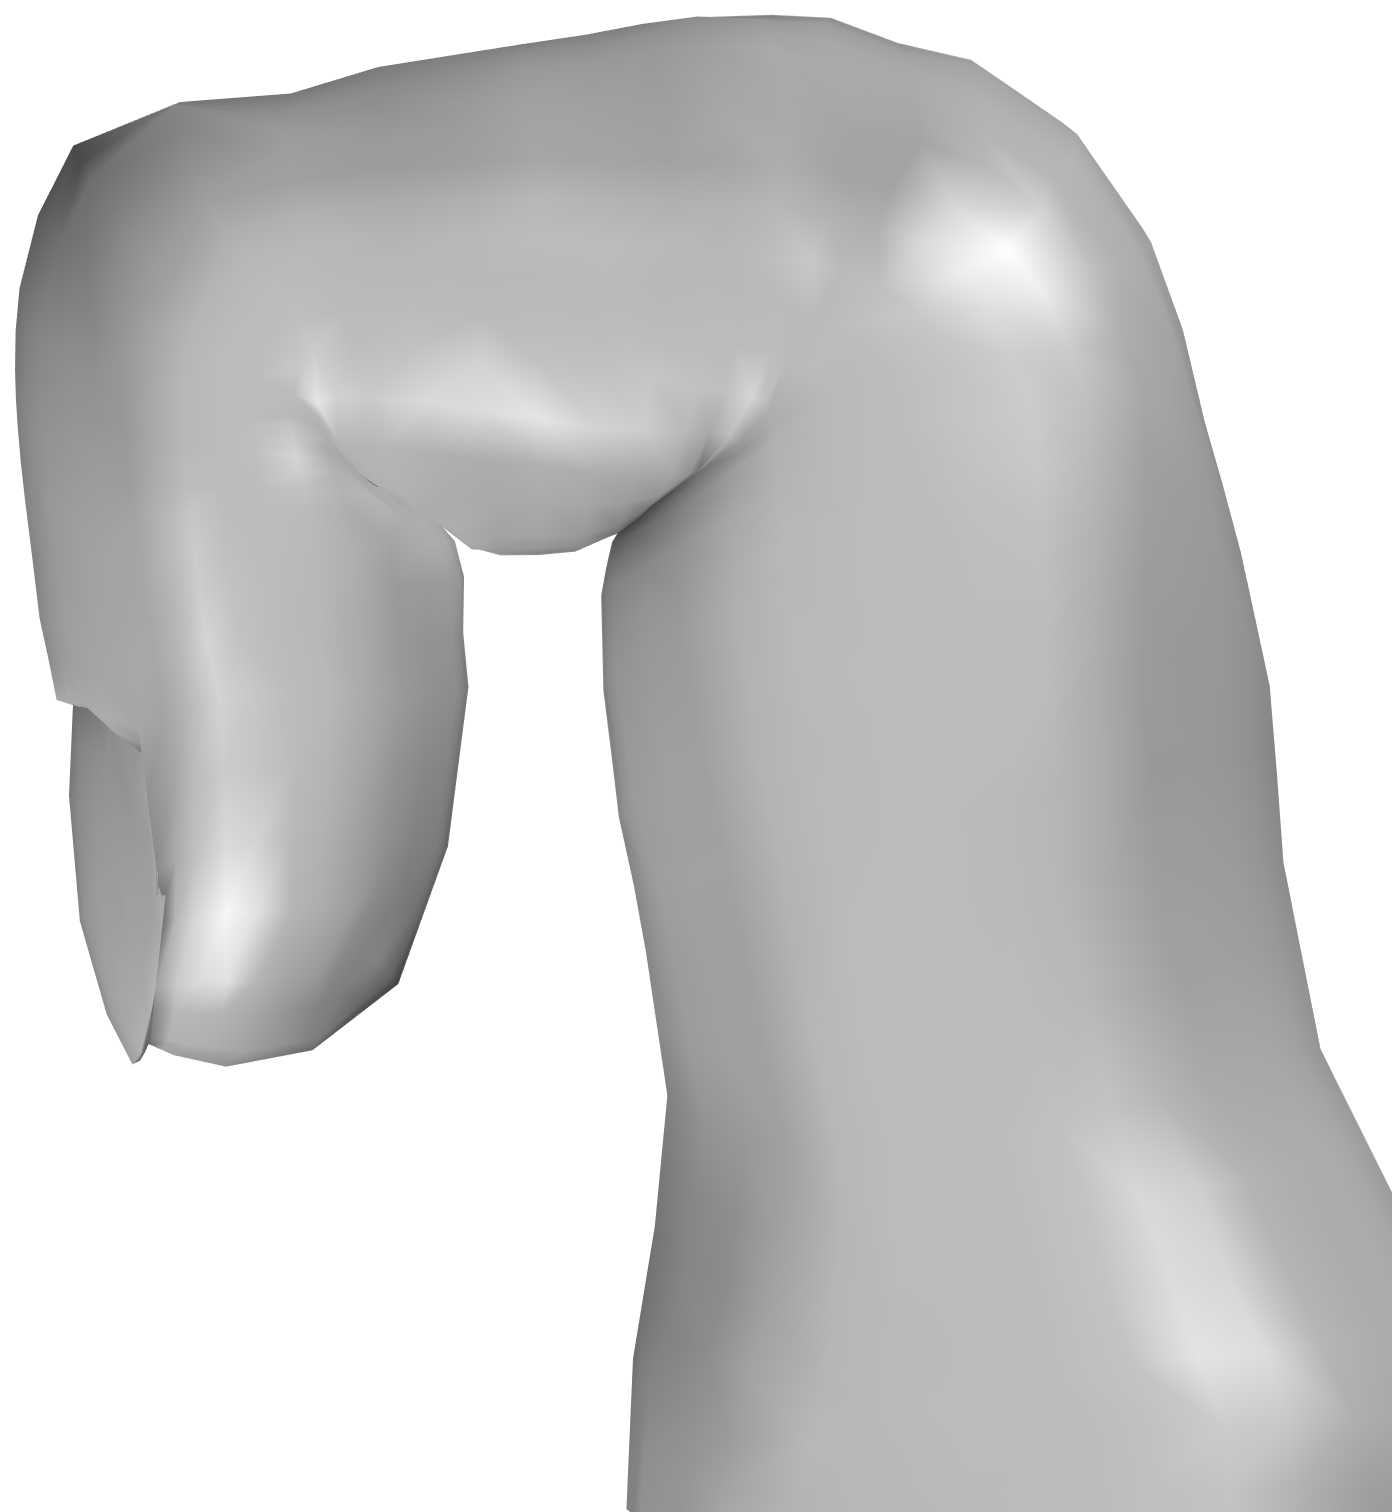
\includegraphics[width=0.14\textwidth]{figs/index_implicit_hrbf}
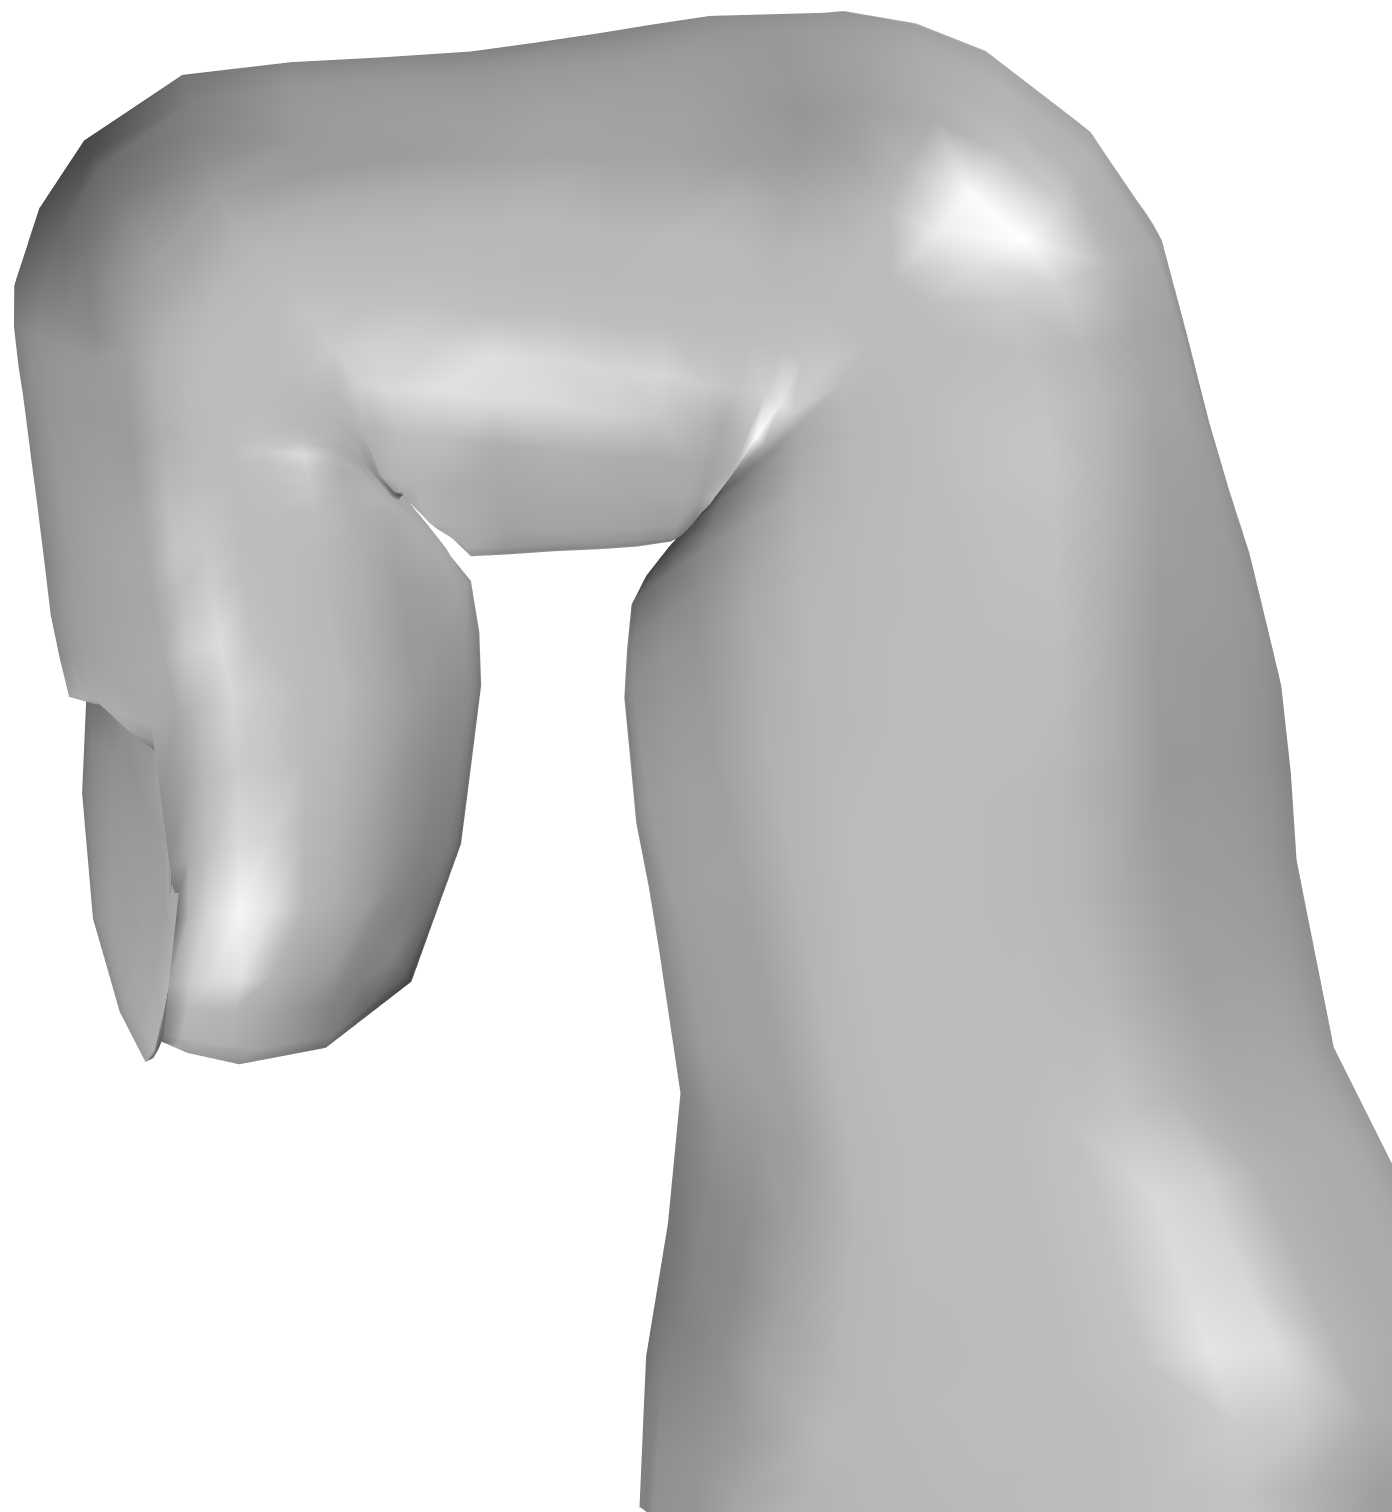
\includegraphics[width=0.14\textwidth]{figs/index_implicit_spheres}
\caption{Close view of an index finger deformed using HRBFs (left and middle) and spherical primitives (right).
The top row shows the reconstructed surfaces, combined with the union operator.
The leftmost column is showing the results with poorly adjusted HRBFs, while the column in the middle has a smoother surface because we tweaked the HRBFs.}
\end{figure}

However, in the interior side, the mesh is more appealing when using HRBFs, because the bulge effect is more visible.
This is caused by the spherical primitives producing a flat surface in-between the spheres, thus projecting all the vertices in the same direction.

In some poses, the spherical primitives can also suffer from the problem of surfaces non smoothly joining.
Indeed, the wrist, the palm and the bases of the thumb and the little finger are composed of flat surfaces.
So it can happen that these surfaces are misaligned.
This is demonstrated in the following figure, where we can see a bump near the wrist.

\begin{figure}[H]
\centering
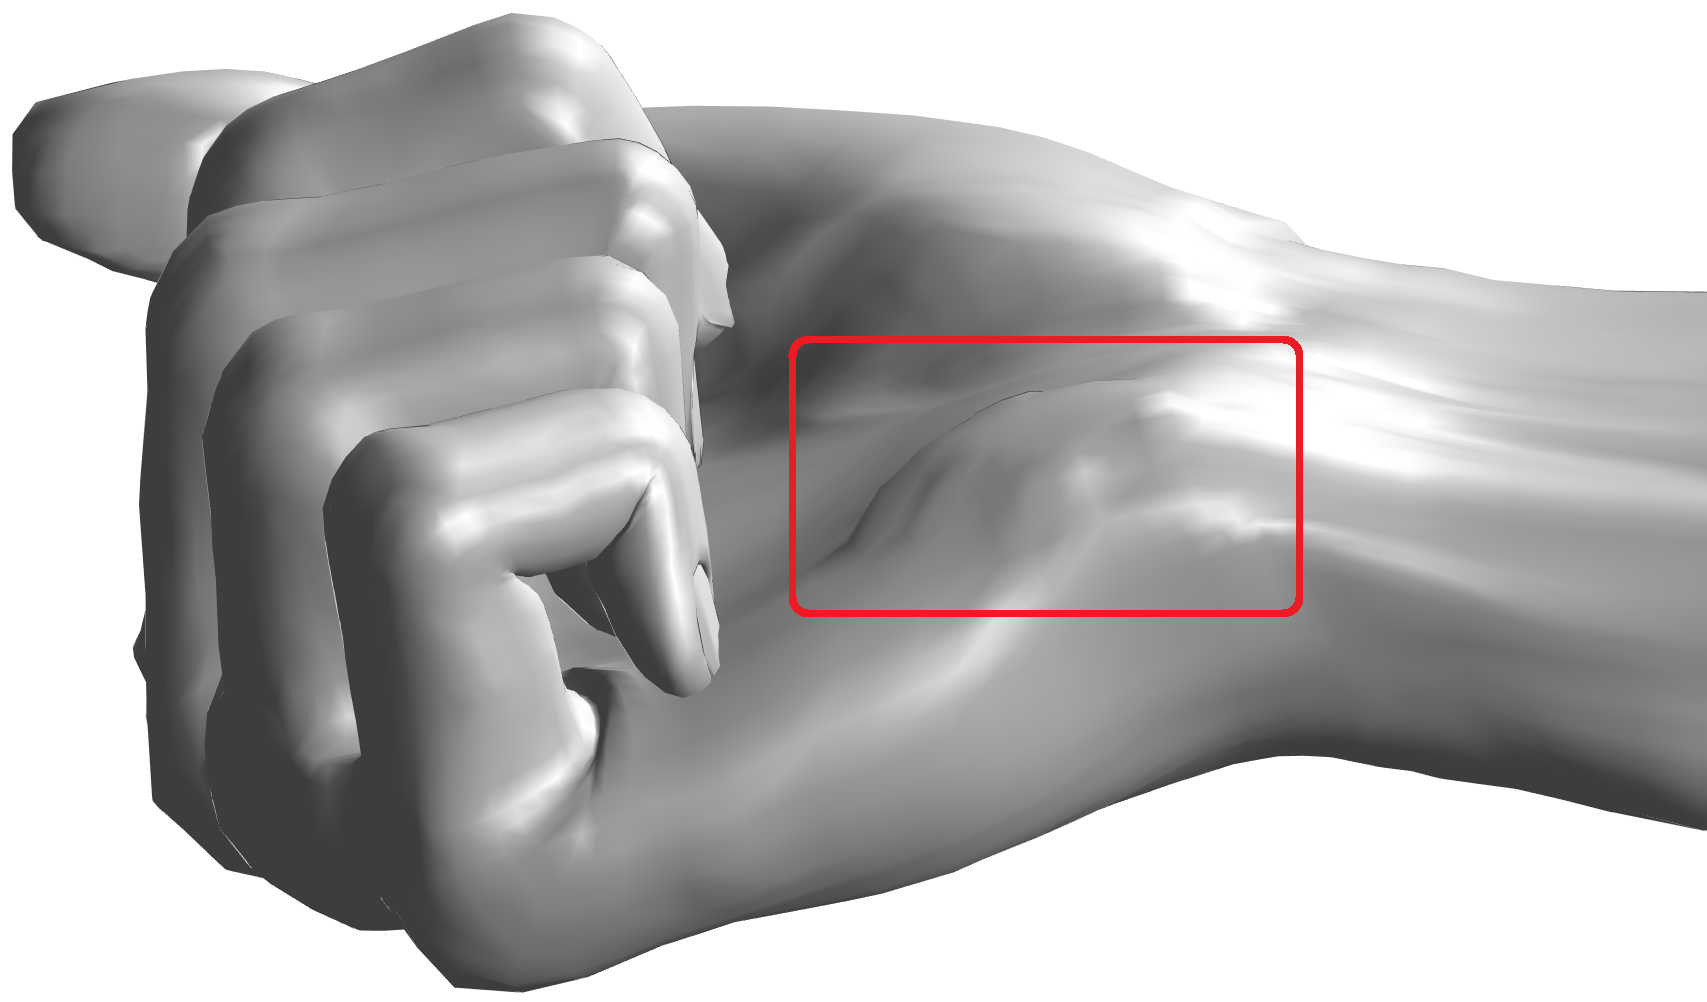
\includegraphics[width=0.45\textwidth]{figs/palm_implicit}
\caption{A hand animated with spherical primitives.}
\end{figure}

During animation, the choice of the geometric skinning method used to get an initial deformation is one of the parameters that can be used to influence the result.
We support linear blending and dual quaternion, but other techniques could easily be plugged in.
By default, we use dual quaternion skinning because it does not suffer from the candy wrapper effect and it is less likely to produce deep self-intersections.
As illustrated in the following figure, self-intersections could lead to projections in the wrong direction.

\begin{figure}[H]
\centering
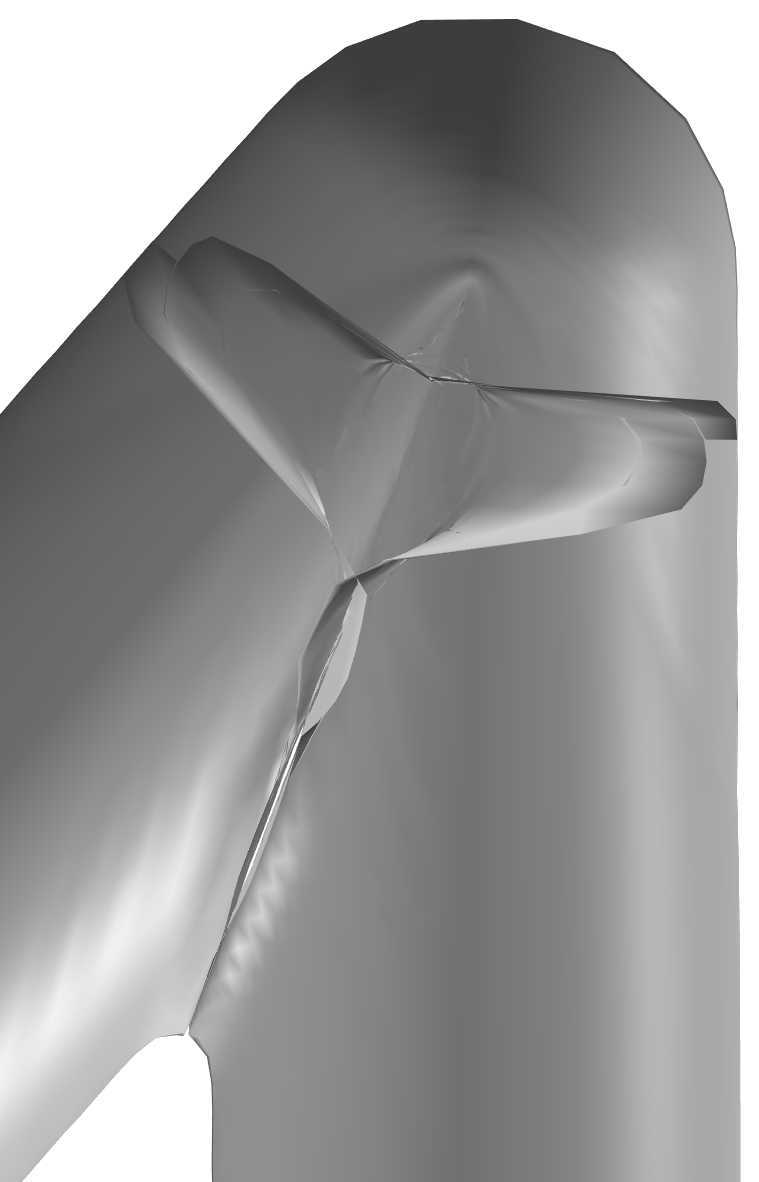
\includegraphics[width=0.17\textwidth]{figs/cylinder_linear_self}
\qquad
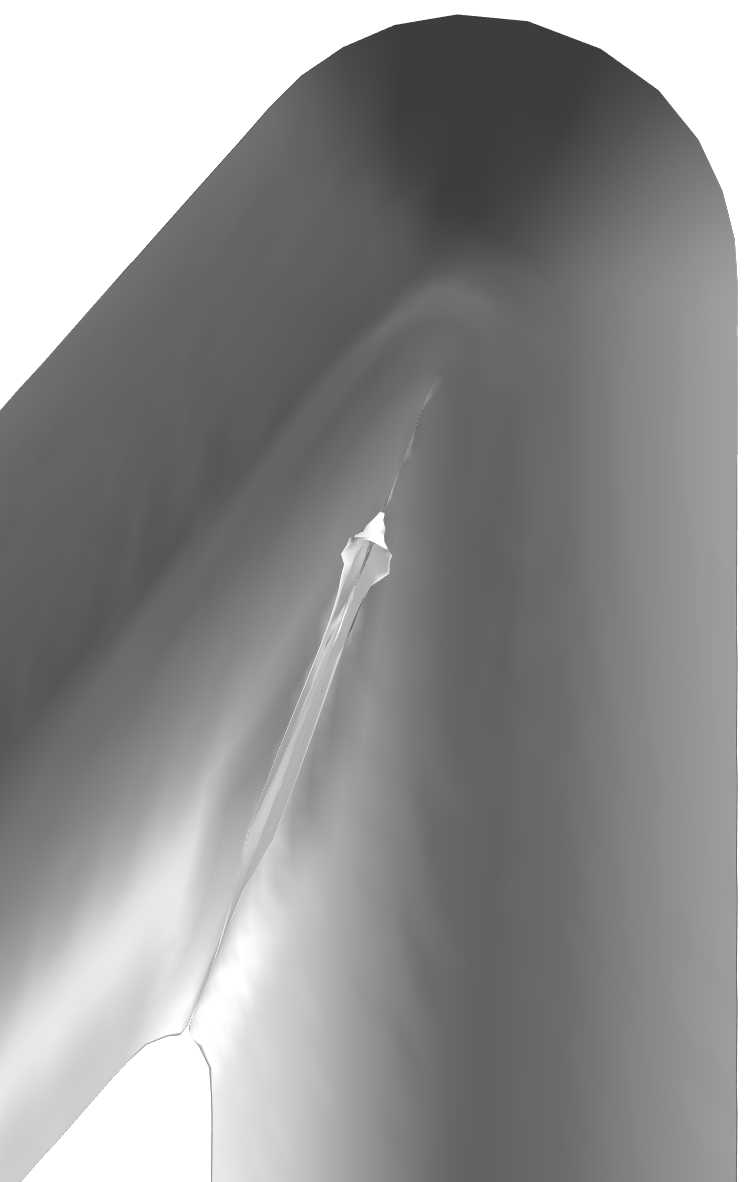
\includegraphics[width=0.17\textwidth]{figs/cylinder_dualquat_self}
\caption{When the initial mesh deformation is produced by linear blend skinning (left), this section of a cylinder exhibits artifacts because some vertices were projected on the wrong side.
With dual quaternion (right), the vertex projection works correctly because the vertices are on the correct side of the implicit surfaces.}
\end{figure}

Another parameter is the reparametrization distance used to convert the fields with global supports into locally supported fields.
Its effect is to increase or decrease the bulge, as we can see in the following figure where thresholds of $1$, $2$ and $3$ were used.

\begin{figure}[H]
\centering
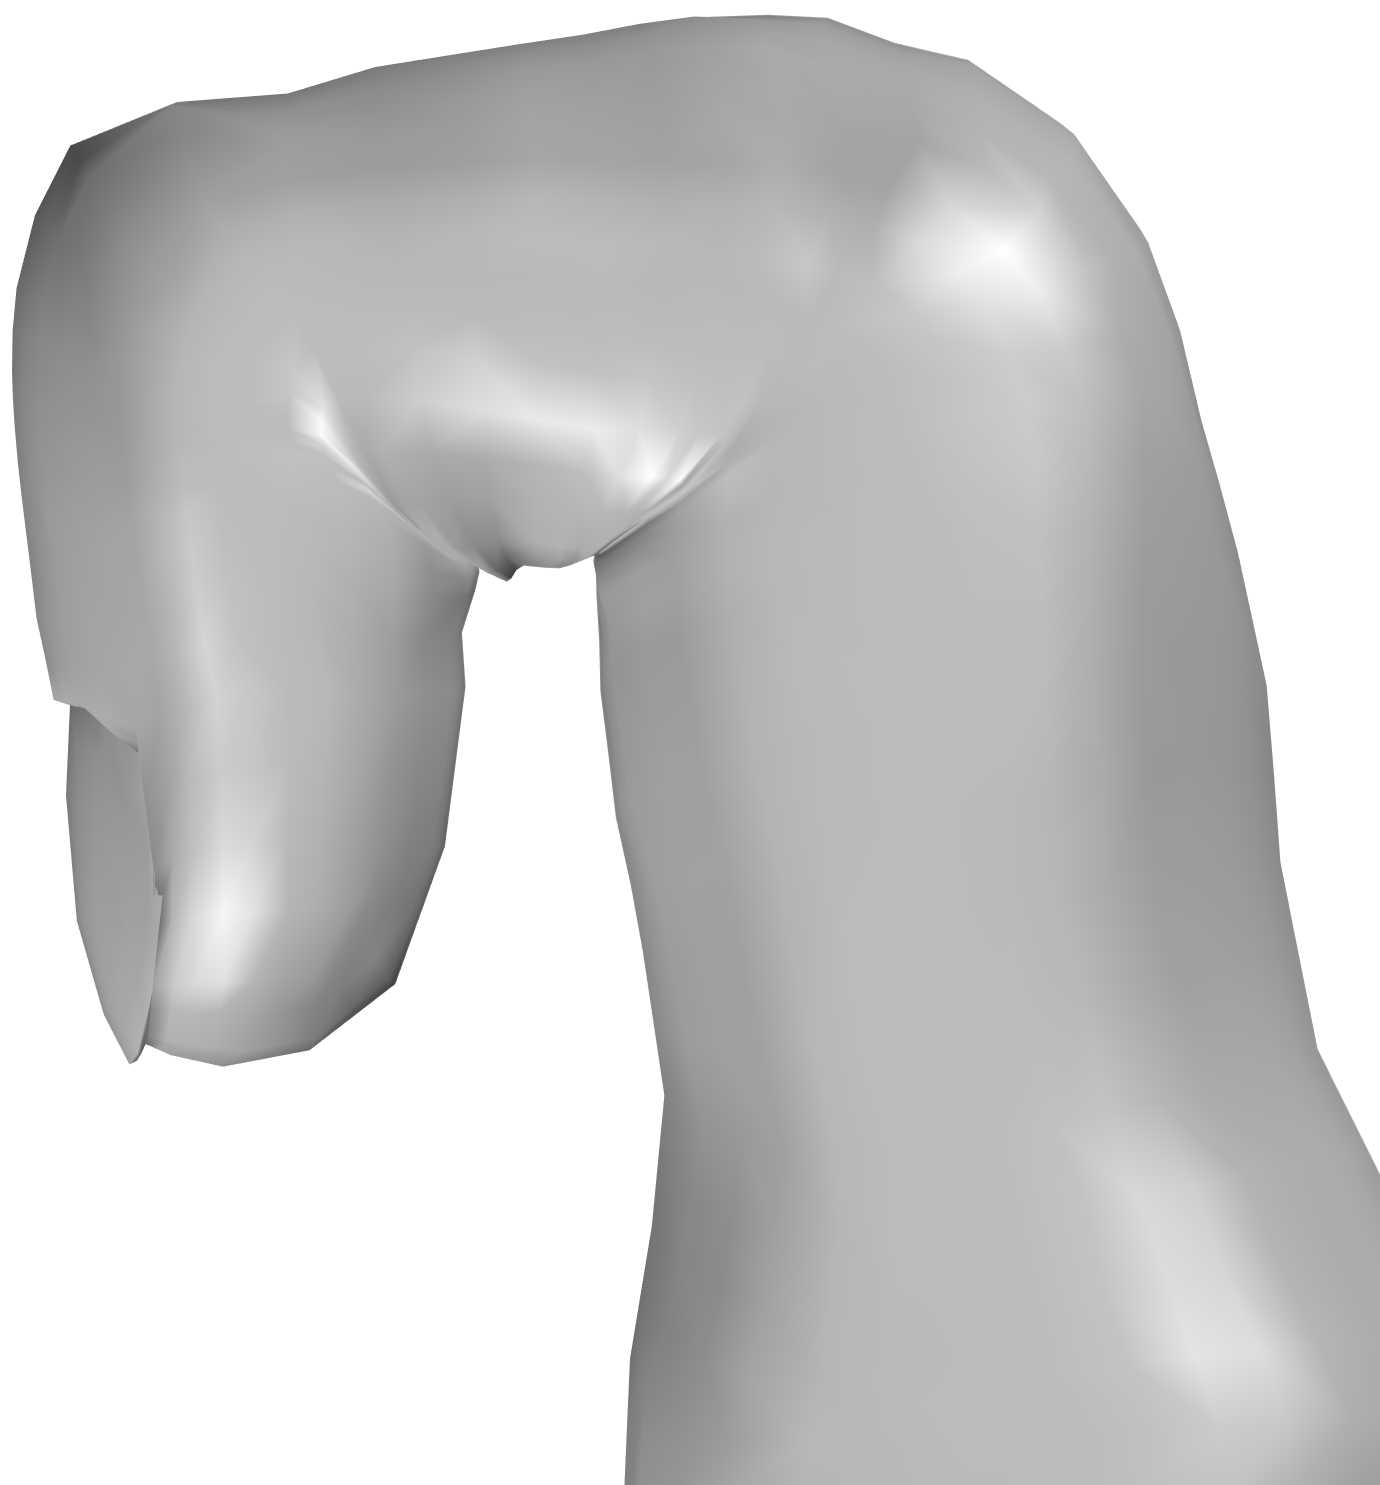
\includegraphics[width=0.15\textwidth]{figs/index_implicit_thresh1}
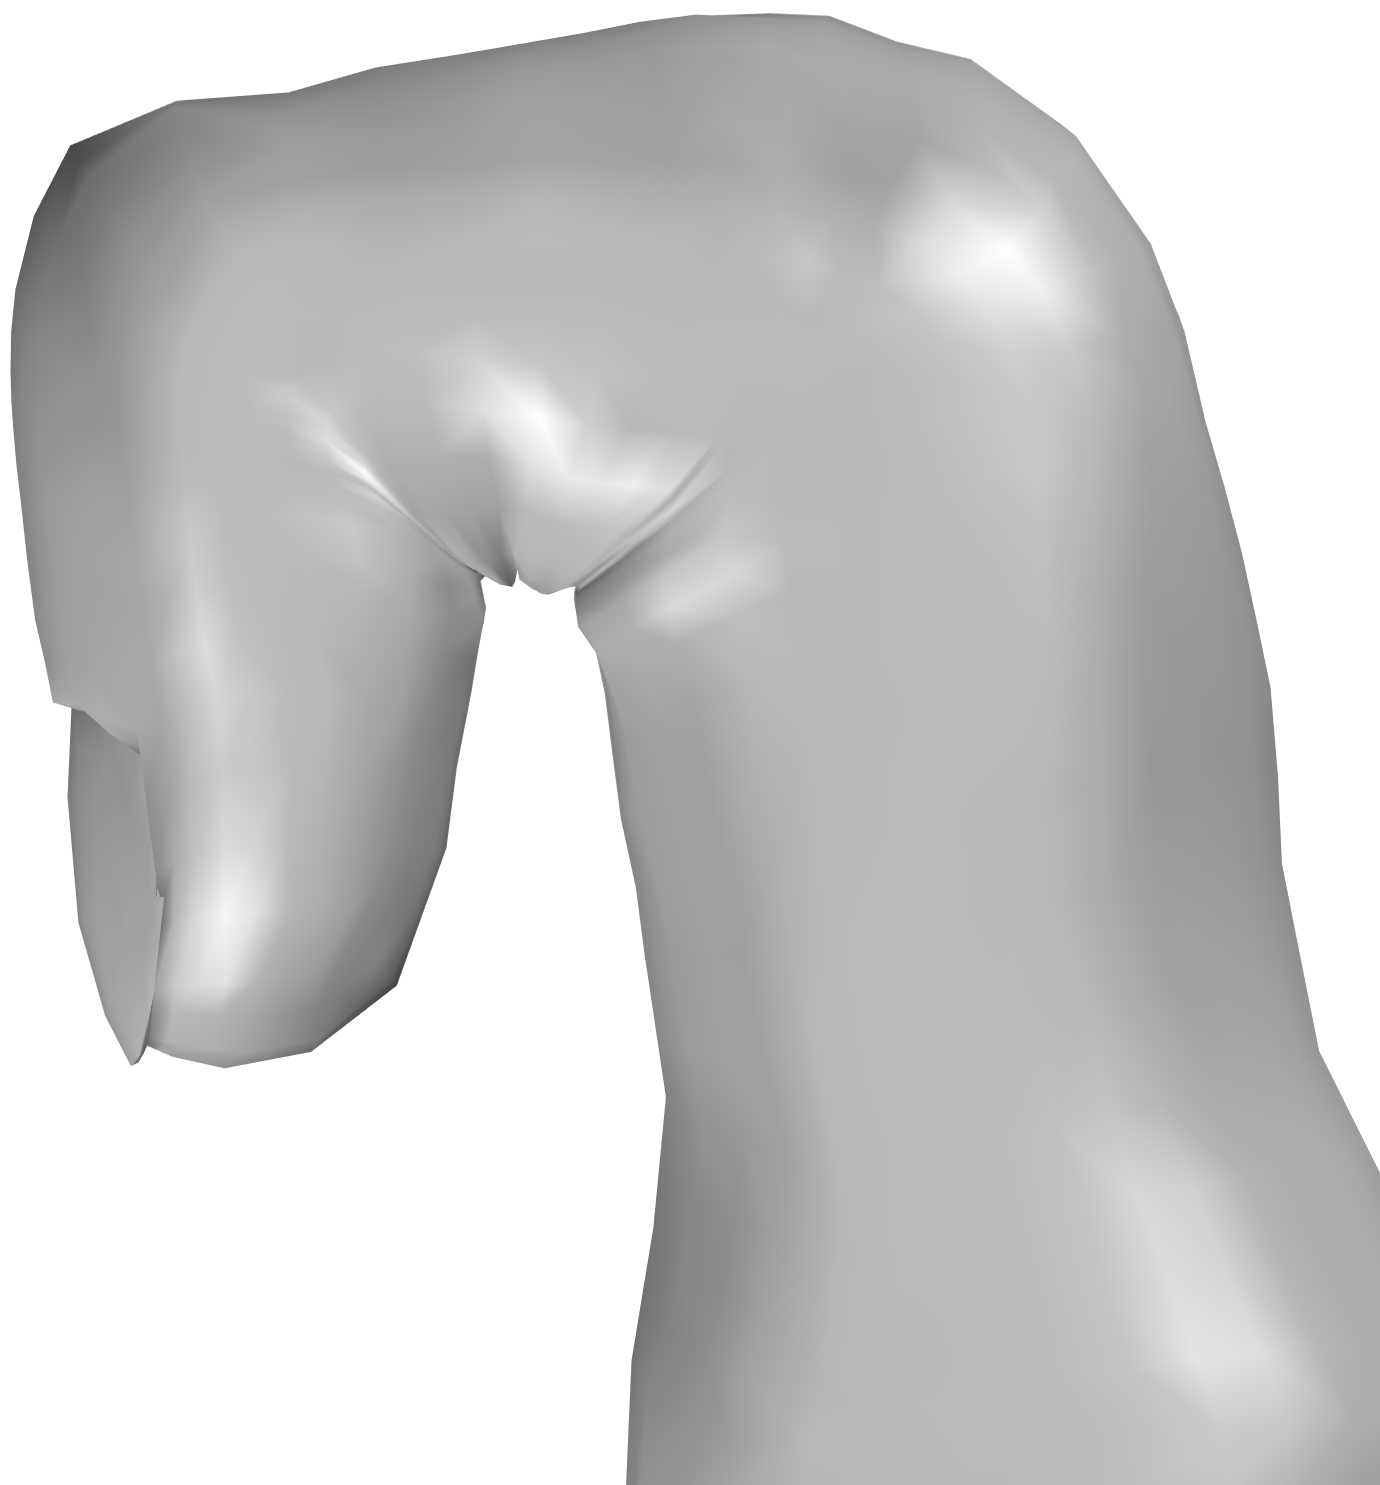
\includegraphics[width=0.15\textwidth]{figs/index_implicit_thresh2}
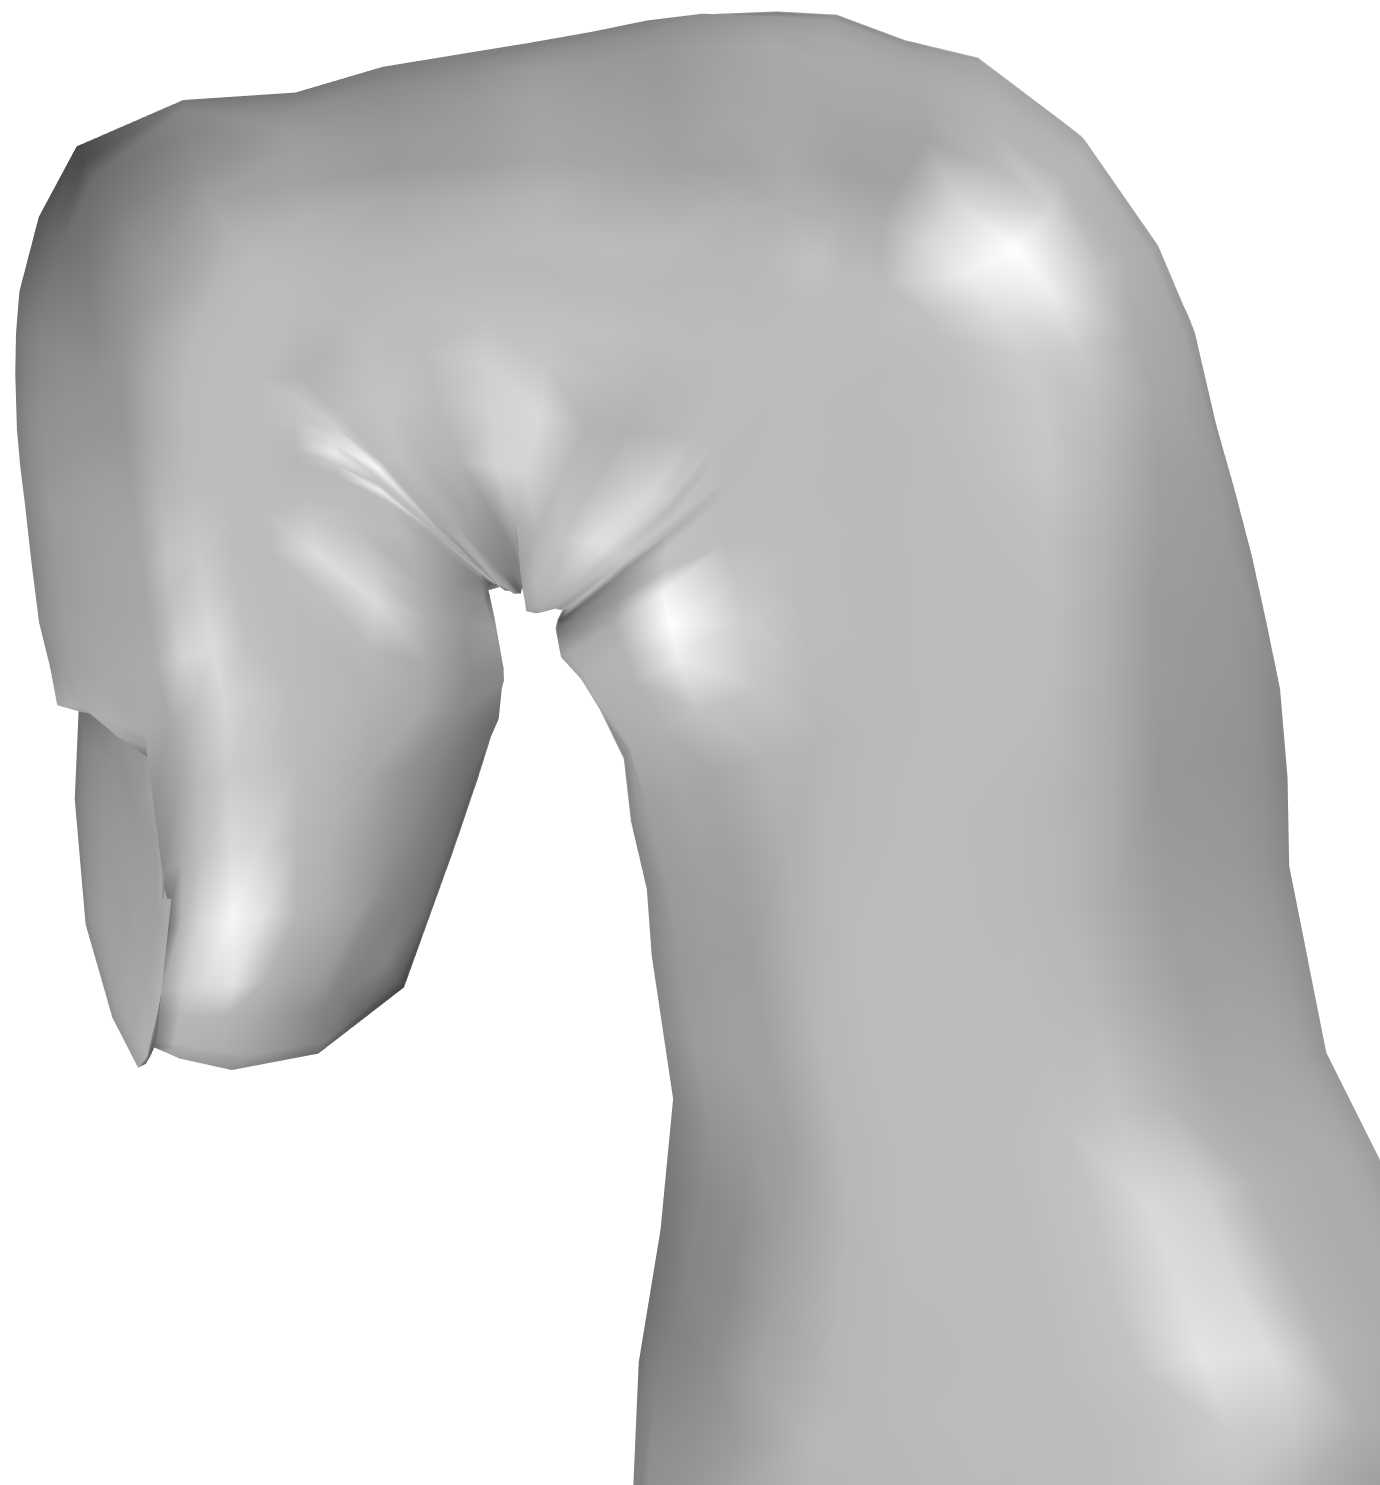
\includegraphics[width=0.15\textwidth]{figs/index_implicit_thresh3}
\caption{Index finger deformed while varying the threshold.
We can see that the muscular bulges inflate as the threshold increases.}
\end{figure}

Fine control over the bulge effect is provided by the 8 arguments of the function $\theta(\alpha)$.
They can be changed to model different types of material, like rubber or skin.
Because it is quite tedious to set these correctly and because we were interested only in hand deformations, we generally used the parameters shown in figure \ref{fig:theta}.

Finally, in order to avoid creating bulges on the exterior side of fingers, we added a parameter the we call \emph{blending weights}.
They are used to linearly interpolate between union and blend.
As illustrated in the following figure, we set the weights close to $1$ in the inner part of the fingers while the exterior side is set to $0$.
The advantage is that the use of the weights creates a really smooth field, allowing for realistic rendering.
On the other hand, an unexpected side effect of the interpolation is that it drastically reduces the influence of other parameters.

\begin{figure}[H]
\centering
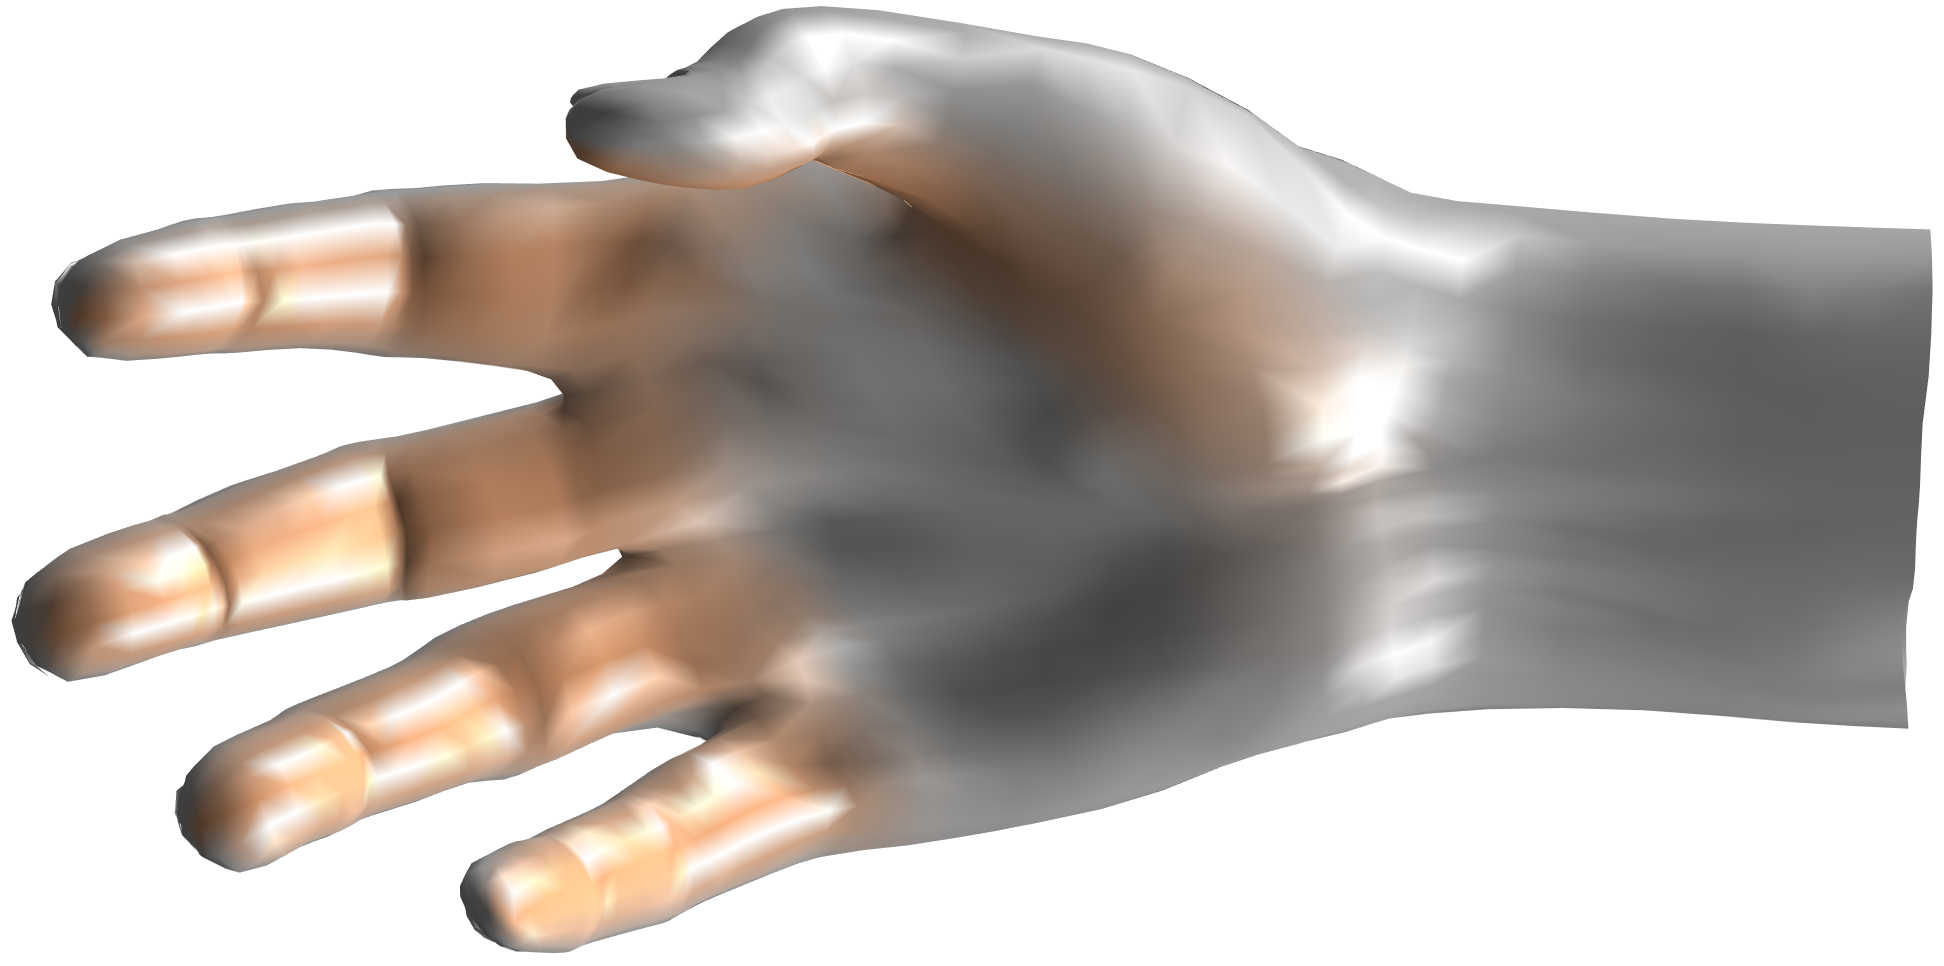
\includegraphics[width=0.45\textwidth]{figs/hand_bone_blend_weights}
\caption{Illustration of the blending weights on the hand.
The intensity of orange indicates the strength with which we apply the blend operator.}
\end{figure}

We implemented implicit skinning both in MatLab and C++.
In MatLab, all the functions are vectorized over the vertices, allowing for decent performances (not real-time though).
We compared the versions using a low polygon mesh and with a tessellated mesh.
The low-resolution mesh has $3\ 045$ vertices while the high-resolution has $12\ 125$ vertices.
It should be noted that the C++ version only supports the union operator and HRBFs, so we tested the MatLab version both with these settings and with the bulge operator for the fingers.

\begin{table}[H]
\centering
\begin{tabular}{ l | c c c }
  & HRBF & Spheres & DQS \\
  \hline
  ML low-res & 3.0s & 5.6s & 15ms \\
  ML high-res & 5.9s & 10.6s & 90ms \\
  ML low (union) & 0.75s & 1.4s & - \\
  ML high (union) & 1.45s & 2.15s & -\\
  C++ low-res & 13ms & - & 1.5ms \\
  C++ high-res & 55ms & - & 1.7ms
\end{tabular}
\caption{Comparison of the time to compute one animation in MatLab and in C++.}
\end{table}

\section{Conclusion}

As we can see in our results, implicit skinning has significative visual improvements over dual quaternion skinning.
Even if no bulge effect is applied, using only the union operator fixes vertices distances to bones.
Soft bodies that rely on a rigid skeleton benefit from this algorithm and display more realistic behaviour.
The blend operator and the versatile nature of isosurfaces combination makes Implicit skinning a promising asset in computer graphics.

For clarity's sake, both our codes use straightforward implementations.
Hence, many optimization opportunities are left.
Profiling our code revealed that the most time-consuming task is signed distance function evaluation.
Precomputing and caching these values would probably dramatically improves performances.
However, code readability is a major goal of our project.

As Vaillant suggests, GPU implementation is required to achieve maximal framerate.
Due to the iterative nature of the method, parallelization is not as trivial as in linear blend or dual quaternion skinning.
Each tangential relaxation step requires the locations of neighboring vertices.
This memory barrier might be the bottleneck in a distributed implementation.

Our implementation also suffers from some minor issues.
As previously discussed, many parameters must be finely tuned in order to provide realistic results.
Skinning weights, HRBF coefficients and reparametrization threshold can still be improved.
Moreover, some heuristics could be enhanced, such as bone transforms estimation from spheres.
The thumb orientation in highly curved poses might be inaccurately reproduced.

In conclusion, implicit skinning is a powerful tool that requires more care than usual skinning techniques.
As it enforces rigid transformation more tightly, it is especially suited for hand animation.
With appropriate optimizations, this algorithm provides real-time animations that requires realistic results.


\section*{Acknowledgments}

This work was done as a semester project, for our Master in Computer Science at the École Polytechnique Fédérale de Lausanne, Switzerland.
We thank Anastasia Tkach and Mark Pauly for their support during the whole semester.
We also thank Alec Jacobson for his amazing MatLab toolbox \cite{gptoolbox}.


\appendix

\section{Matrix calculus}
\label{section:calculus}

To avoid tedious details during explanations, mathematical expressions of basic building blocks will be described here.
Most of the derivations can be formulated using matrices and are based on both analysis and geometrical results.
While common calculus concepts work as expected, such as derivative chain rule, most complex cases need some care in order to produce clean expressions.

\begin{equation*}
\left\| \mathbf{v} \right\| = \sqrt{\mathbf{v}^T\mathbf{v}} \qquad
\frac{\partial}{\partial \mathbf{v}} \left\| \mathbf{v} \right\| = \frac{\mathbf{v}^T}{\left\| \mathbf{v} \right\|} = \overbar{\mathbf{v}}^T
\end{equation*}

\begin{equation*}
\frac{\partial}{\partial \mathbf{v}} \overbar{\mathbf{v}} = 
\frac{1}{\left\| \mathbf{v} \right\|}\left( \mathbf{I}_3 - \frac{\mathbf{v}}{\left\| \mathbf{v} \right\|} \frac{\mathbf{v}^T}{\left\| \mathbf{v} \right\|} \right) =
\frac{\mathbf{I}_3 - \overbar{\mathbf{v}}\overbar{\mathbf{v}}^T}{\left\| \mathbf{v} \right\|}
\end{equation*}

\begin{equation*}
\mathbf{v} \times \mathbf{w} =
\begin{bmatrix}v_y w_z - v_z w_y \\ v_z w_x - v_x w_z \\ v_x w_y - v_y w_x \end{bmatrix} =
\left[\mathbf{w}\right]_\times^T \mathbf{v}
\end{equation*}

\begin{equation*}
\frac{\partial}{\partial \mathbf{v}} \mathbf{v} \times \mathbf{w} =
\begin{bmatrix} 0 & w_z & -w_y \\ w_z & 0 & w_x \\ -w_y & w_x & 0 \end{bmatrix} =
\left[\mathbf{w}\right]_\times
\end{equation*}


\section{Dual quaternion}
\label{section:quaternion}

A \emph{quaternion} is an extension to complex numbers usually used to represent 3D rotations.
While we assume basic knowledge about their definition and usage, expressions required for skinning are described in this appendix.
We adopt the vector notation by packing imaginary components into a vector:

\begin{equation*}
\mathbf{q} = \begin{bmatrix}q_s \\ \mathbf{q}_v \end{bmatrix}
\qquad
\mathbf{q} + \mathbf{r} = \begin{bmatrix}q_s + r_s \\ \mathbf{q}_v + \mathbf{r}_v \end{bmatrix}
\end{equation*}

\begin{equation*}
\mathbf{q} \mathbf{r} = \begin{bmatrix}q_s r_s - \mathbf{q}_v^T \mathbf{r}_v \\ q_s\mathbf{r}_v + r_s\mathbf{q}_v + \mathbf{q}_v \times \mathbf{r}_v \end{bmatrix}
\end{equation*}

The conjugate is used to define the norm:

\begin{equation*}
\mathbf{q}^* = \begin{bmatrix}q_s \\ -\mathbf{q}_v \end{bmatrix}
\qquad
\left\|\mathbf{q}\right\| = \sqrt{\mathbf{q}\mathbf{q}^*}
\qquad
\overbar{\mathbf{q}} = \frac{\mathbf{q}}{\left\|\mathbf{q}\right\|}
\end{equation*}

\emph{Unit quaternions} have a length of $1$ and are used to represent any rotation.
A vector $\mathbf{v}$ is transformed by a unit quaternion $\mathbf{q}$ as follows:

\begin{equation*}
\begin{bmatrix}0 \\ \mathbf{v}' \end{bmatrix} = \mathbf{q} \begin{bmatrix}0 \\ \mathbf{v} \end{bmatrix} \mathbf{q} ^*
\end{equation*}

To represent translations as well, \emph{dual quaternions} can be used, which are a pair of quaternions.
Again, details about \emph{dual numbers} will not be covered in this document.
As a reminder, the \emph{dual operator} $\varepsilon$ is defined such that $\varepsilon^2 = 0$, but $\varepsilon \not= 0$.
Quaternion arithmetics is unchanged:

\begin{equation*}
\mathbf{d} = \mathbf{d}_r + \mathbf{d}_d \varepsilon
\qquad
\mathbf{d} + \mathbf{e} = \mathbf{d}_r + \mathbf{e}_r + \left( \mathbf{d}_d + \mathbf{e}_d\right) \varepsilon
\end{equation*}

\begin{equation*}
\mathbf{d} \mathbf{e} = \mathbf{d}_r \mathbf{e}_r + \left( \mathbf{d}_r \mathbf{e}_d + \mathbf{d}_d \mathbf{e}_r \right)\varepsilon
\end{equation*}

\begin{equation*}
\mathbf{d}^* = \mathbf{d}_r^* + \mathbf{d}_d^* \varepsilon
\qquad
\left\|\mathbf{d}\right\| = \sqrt{\mathbf{d}\mathbf{d}^*}
\qquad
\overbar{\mathbf{d}} = \frac{\mathbf{d}}{\left\|\mathbf{d}_r\right\|}
\end{equation*}

A point $\mathbf{v}$ can be represented by the following dual quaternion:
\begin{equation*}
\hat{\mathbf{v}} = \begin{bmatrix}1 \\ \mathbf{0} \end{bmatrix} + \begin{bmatrix}0 \\ \mathbf{v} \end{bmatrix} \varepsilon
\end{equation*}

The dual quaternion $\mathbf{d}$ associated to rotation $\mathbf{q}$ and translation $\mathbf{t}$ is given by:

\begin{equation*}
\mathbf{d} = \mathbf{q} + \frac{1}{2} \mathbf{q} \begin{bmatrix}0 \\ \mathbf{t} \end{bmatrix} \varepsilon
\qquad
\hat{\mathbf{v}}' = \begin{bmatrix}1 \\ \mathbf{0} \end{bmatrix} + \begin{bmatrix}0 \\ \mathbf{v}' \end{bmatrix} \varepsilon = \mathbf{d} \hat{\mathbf{v}} \mathbf{d} ^*
\end{equation*} % For reference: http://www.dsi.unive.it/~rodola/cvpr11-dual.pdf


\section{Quadratic programming}
\label{section:quadratic}

In convex optimization, a \emph{quadratic program} with \emph{linear equality constraints} can be represented as:

\begin{equation*}
\begin{aligned}
& \underset{\mathbf{x}}{\text{minimize}} & & \frac{1}{2} \mathbf{x}^T \mathbf{Q} \mathbf{x} + \mathbf{c}^T \mathbf{x} \\
& \text{subject to} & & \mathbf{E}\mathbf{x} = \mathbf{d}
\end{aligned}
\end{equation*}

The solution can be found by solving the \emph{equilibrium equations}:

\begin{equation*}
\begin{bmatrix} \mathbf{Q} & \mathbf{E}^T \\ \mathbf{E} & \mathbf{0} \end{bmatrix}
\begin{bmatrix} \mathbf{x} \\ \boldsymbol\lambda \end{bmatrix} =
\begin{bmatrix} - \mathbf{c} \\ \mathbf{d} \end{bmatrix}
\end{equation*}

Since we usually deal with energy minimization, the following least square formulation is more appropriated, where the first $h$ variables are constrained

\begin{equation*}
\begin{aligned}
& \underset{\mathbf{x}}{\text{minimize}} & & \frac{1}{2} \sum_c w_c \left\| \mathbf{A}_c\mathbf{x} \right\|_2^2 \\
& \text{subject to} & & x_i = x_i^* \qquad i = {1, ..., h}
\end{aligned}
\end{equation*}

This program can be solved by using:

\begin{equation*}
\mathbf{Q}=\sum_c w_c \mathbf{A}_c^T\mathbf{A}_c
\end{equation*}
\begin{equation*}
\mathbf{c}=0 \qquad \mathbf{E}=\begin{bmatrix} \mathbf{I}_h & \mathbf{0} \end{bmatrix} \qquad \mathbf{d}=\mathbf{x}^*
\end{equation*}


\section{MatLab code}

\lstset{language=MatLab}

In this appendix, the MatLab implementation will be discussed and explained.
Some examples will be presented to provide an overview of the work.
Implementation details are available as comments in the source code.

As most of the project relies on geometry processing, the code is designed to handle large amount of data.
MatLab efficiency heavily depends on code vectorization, i.e. applying operations on matrices rather than on individual values.
Therefore, we assume that the reader has some knowledge of MatLab scripting and indexing subtleties.

First, the \emph{Geometry Processing Toolbox}\cite{gptoolbox} by Alec Jacobson must be introduced.
Developed during its PhD, this project has benefited from various collaborators.
Many mesh algorithms are available, combining efficiency and ease-of-use, which makes this library a strong ally in any computer graphics project.

We adopted most of our convention according to \emph{gptoolbox}.
\emph{Vectors} of size $n$ are stored as $1 \times n$ matrices, which is the transpose of the mathematical representation.
\emph{Lists} of size $n$ are collections of scalars or vectors and are stored as $n \times d$ matrices.
\emph{Meshes} in their minimal representation are stored as a list of vertex positions \lstinline!V! and a list of face indices \lstinline!F!.

\begin{lstlisting}
[V, F] = load_mesh('neutral.obj');
\end{lstlisting}
% trimesh(F, ...
% V(:, 1), V(:, 2), V(:, 3), ...
% 'EdgeColor', 'none', ...
% 'FaceColor', [0.8 0.8 0.8]);
% axis equal;
% view([90, 0]);
% camlight;
% lighting gouraud;

\begin{center}
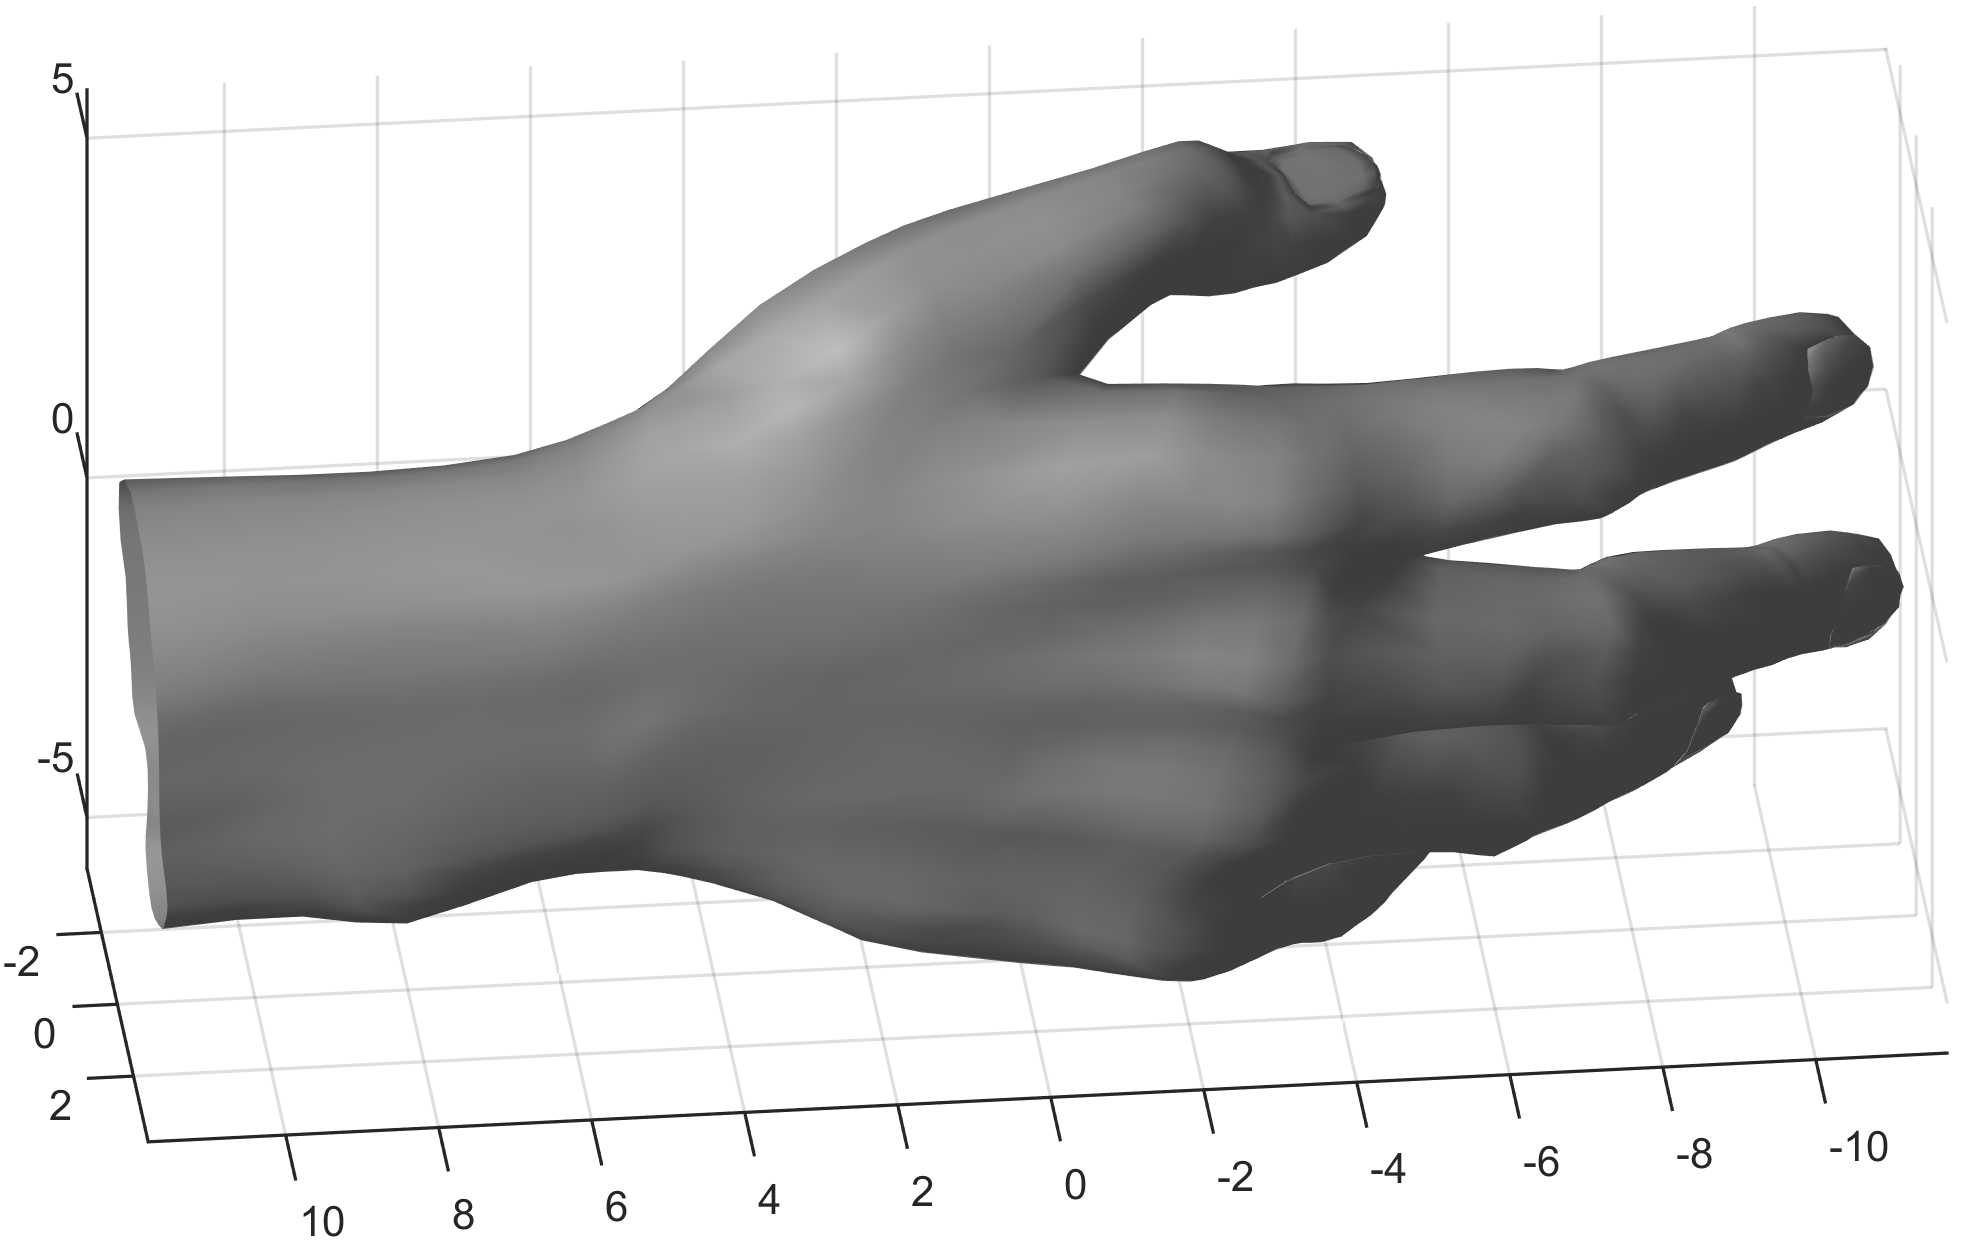
\includegraphics[width=0.45\textwidth]{figs/demo_mesh}
\end{center}


\subsection{Hermite Radial Basis Function}

Poisson sampling over the surface to generate centers and control points is respectively done with \lstinline!hrbf_centers! and \lstinline!hrbf_points!.
The system of equations described in section \ref{section:hrbf} is solved by \lstinline!hrbf_coefficients!.
The following code generate $20$ centers \lstinline!C! and several control points \lstinline!P! and compute HRBF coefficients \lstinline!K!:

\begin{lstlisting}
C = hrbf_centers(V, F, 20);
[P, N] = hrbf_points(V, F);
K = hrbf_coefficients(C, P, N);
\end{lstlisting}

Once this precomputation is done, distance and gradient can be evaluated for any point in space using \lstinline!hrbf_apply!.

\begin{lstlisting}
[D, G] = hrbf_apply(C, K, ...
  [1.0, 0.2, 0.5]);
\end{lstlisting}

As stated before, most functions support vectorized arguments.
As such, multiple points can be queried at once.

\begin{lstlisting}
[X, Y, Z] = meshgrid( ...
  -13.0 : 0.25 : 11.0, ...
  -5.0 : 0.25 : 5.0, ...
  -7.0 : 0.25 : 7.0);
D = hrbf_apply(C, K, ...
  [X(:), Y(:), Z(:)]);
D = reshape(D, size(X));
\end{lstlisting}
% p = patch(isosurface(X, Y, Z, D, 0));
% isonormals(X, Y, Z, D, p);
% p.FaceColor = [0.8, 0.8, 0.8];
% p.EdgeColor = 'none';
% axis equal;
% view([90, 0]);
% camlight;
% lighting gouraud;

\begin{center}
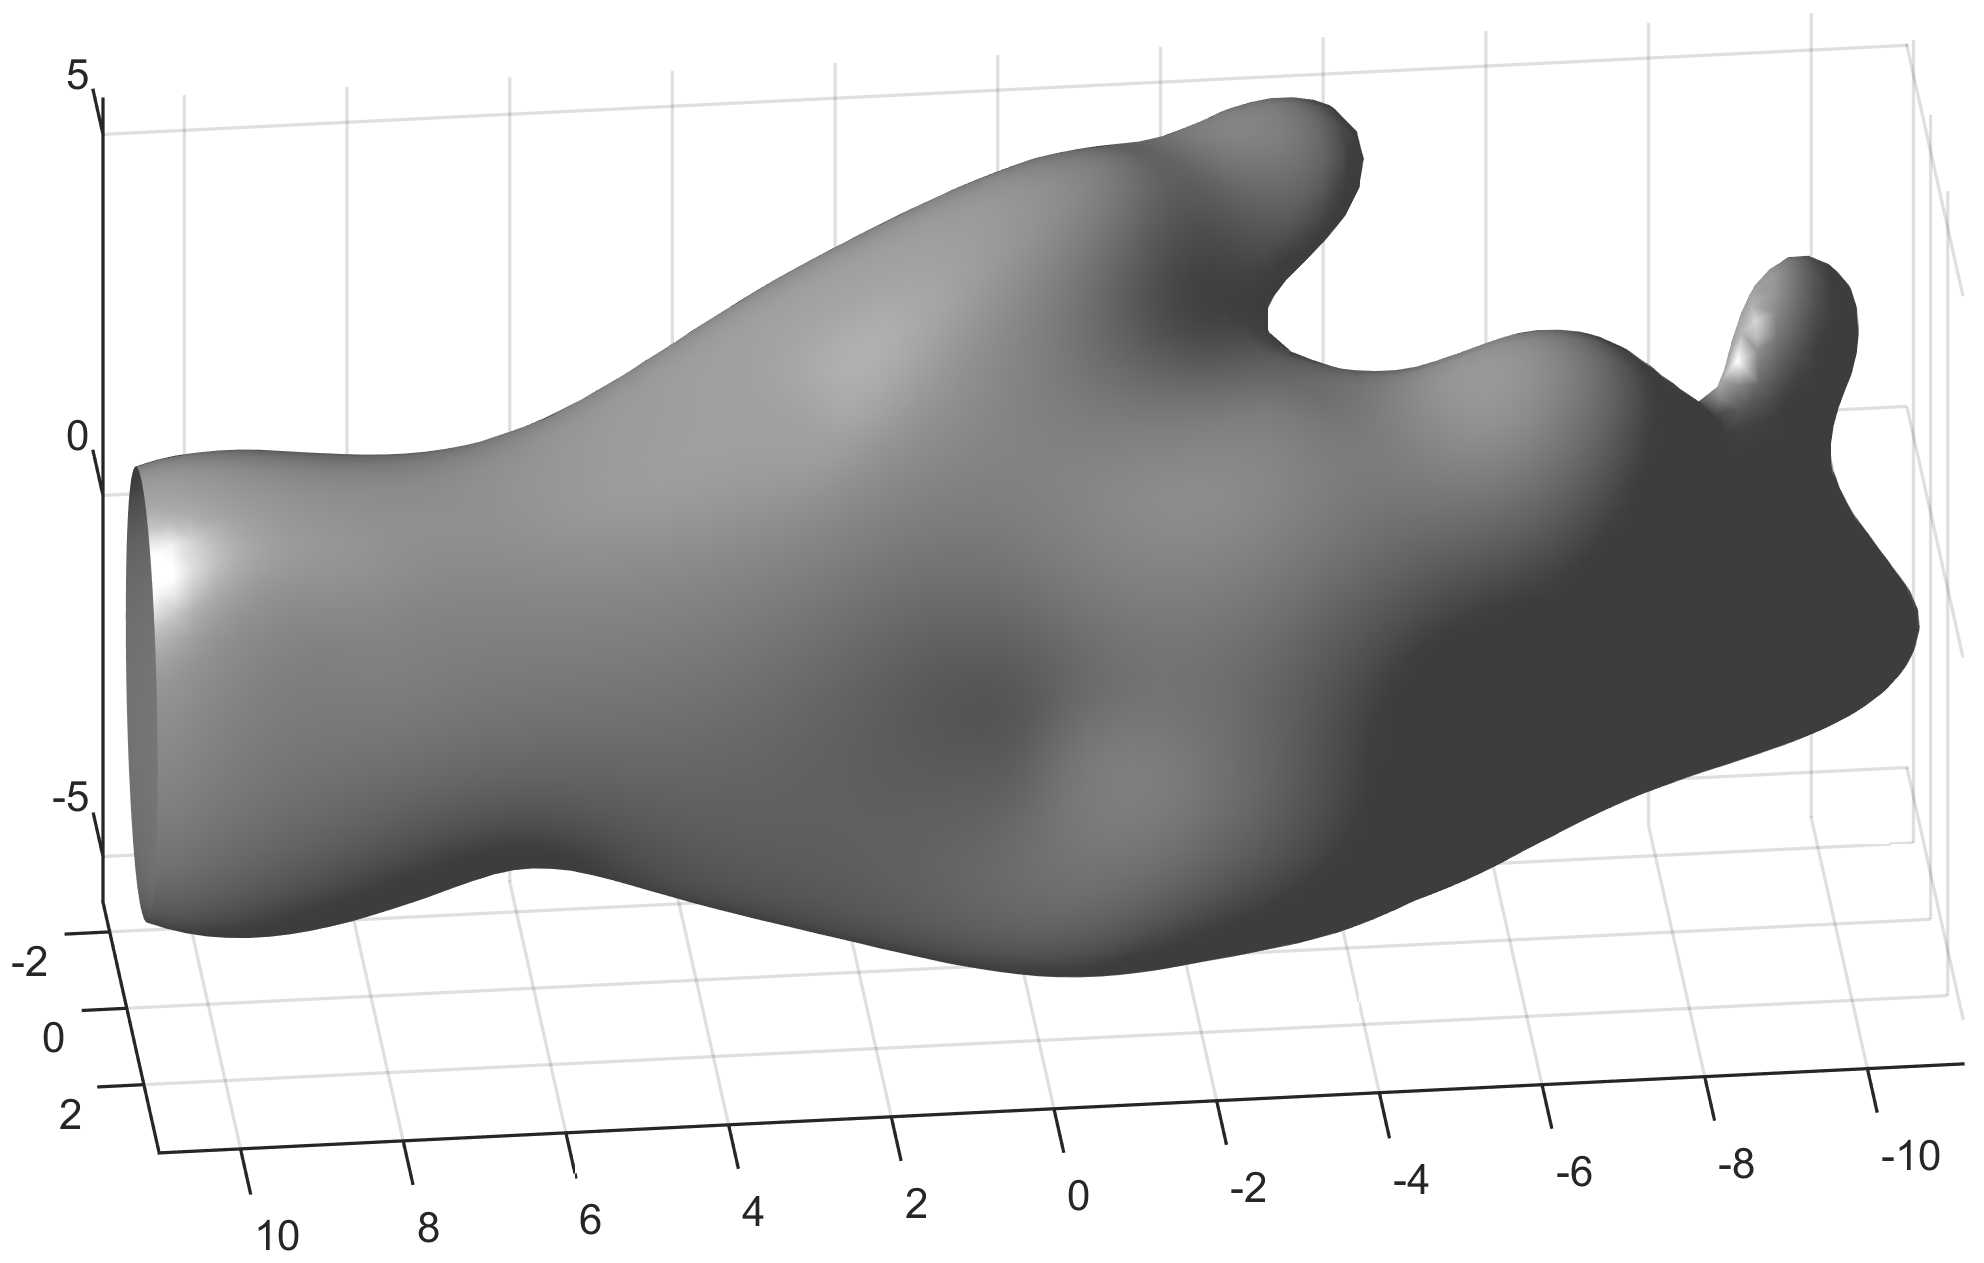
\includegraphics[width=0.45\textwidth]{figs/demo_hrbf}
\end{center}


\subsection{Spherical primitives}

Spheres, bispheres and trispheres are respectively implemented in \lstinline!sphere_single!, \lstinline!sphere_double! and \lstinline!sphere_triple!.
In a similar fashion to \lstinline!hrbf_apply!, these methods compute distances and gradients for given points.

\begin{lstlisting}
[D, G] = sphere_single( ...
  [0.0, 0.0, 0.0], 1.0, ...
  [1.0, 2.0, 3.0]);
\end{lstlisting}

As spherical primitives are usually combined, \lstinline!sphere_apply! takes an array of spheres and an array of indices.

\begin{lstlisting}
S = cell(6, 1);
S{1}.center = [3.0, 2.0, 1.0];
S{1}.radius = 1.0;
S{2}.center = [-2.0, 0.0, 1.5];
S{2}.radius = 2.0;
S{3}.center = [1.0, 1.0, 0.0];
S{3}.radius = 0.5;
S{4}.center = [0.0, 0.0, 3.0];
S{4}.radius = 0.8;
S{5}.center = [0.0, 0.0, -2.0];
S{5}.radius = 1.5;
S{6}.center = [1.0, -3.0, 1.0];
S{6}.radius = 1.2;
I = cell(3, 1);
I{1} = [1];
I{2} = [2, 3];
I{3} = [4, 5, 6];
[X, Y, Z] = meshgrid( ...
  -5.0 : 0.25 : 5.0, ...
  -5.0 : 0.25 : 5.0, ...
  -5.0 : 0.25 : 5.0);
D = sphere_apply(S, I, ...
  [X(:), Y(:), Z(:)]);
D = reshape(D, size(X));
\end{lstlisting}

\begin{center}
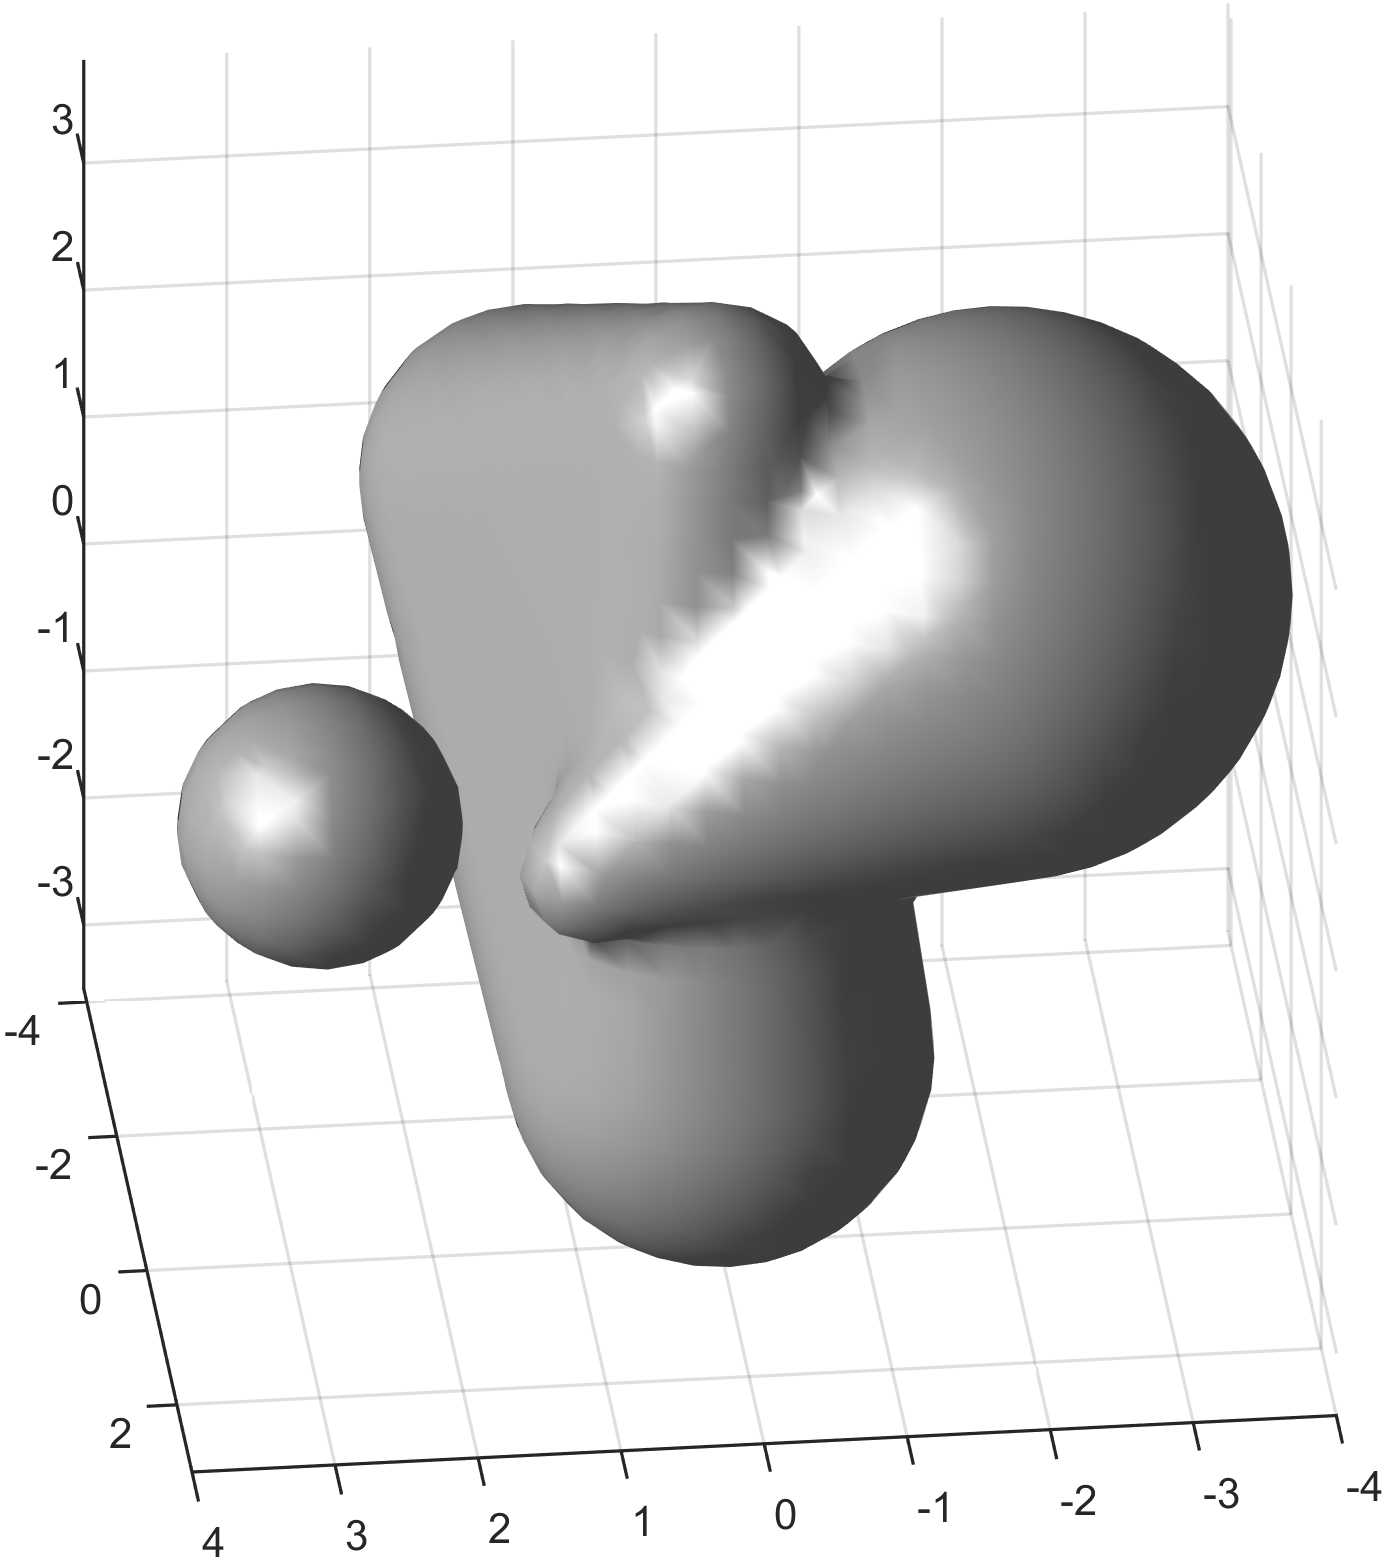
\includegraphics[width=0.3\textwidth]{figs/demo_sphere}
\end{center}


\subsection{Operators}

The function \lstinline!sdf_reparam! converts global distance to local distance.
The union operator is implemented in \lstinline!sdf_union!.

\begin{lstlisting}
[X, Y, Z] = meshgrid( ...
  -3.0 : 0.1 : 5.0, ...
  -2.0 : 0.1 : 5.0, ...
  -5.0 : 0.1 : 5.0);
D1 = sphere_double( ...
  [0.0, 0.0, 1.0], 0.5, ...
  [3.0, -1.0, 2.0], 0.8, ...
  [X(:), Y(:), Z(:)]);
D2 = sphere_double( ...
  [3.0, -1.0, 2.0], 0.8, ...
  [4.0, 0.0, 0.0], 1.0, ...
  [X(:), Y(:), Z(:)]);
D1 = sdf_reparam(D1, 2);
D2 = sdf_reparam(D2, 2);
D = sdf_union(D1, D2);
D = reshape(D, size(X));
\end{lstlisting}

\begin{center}
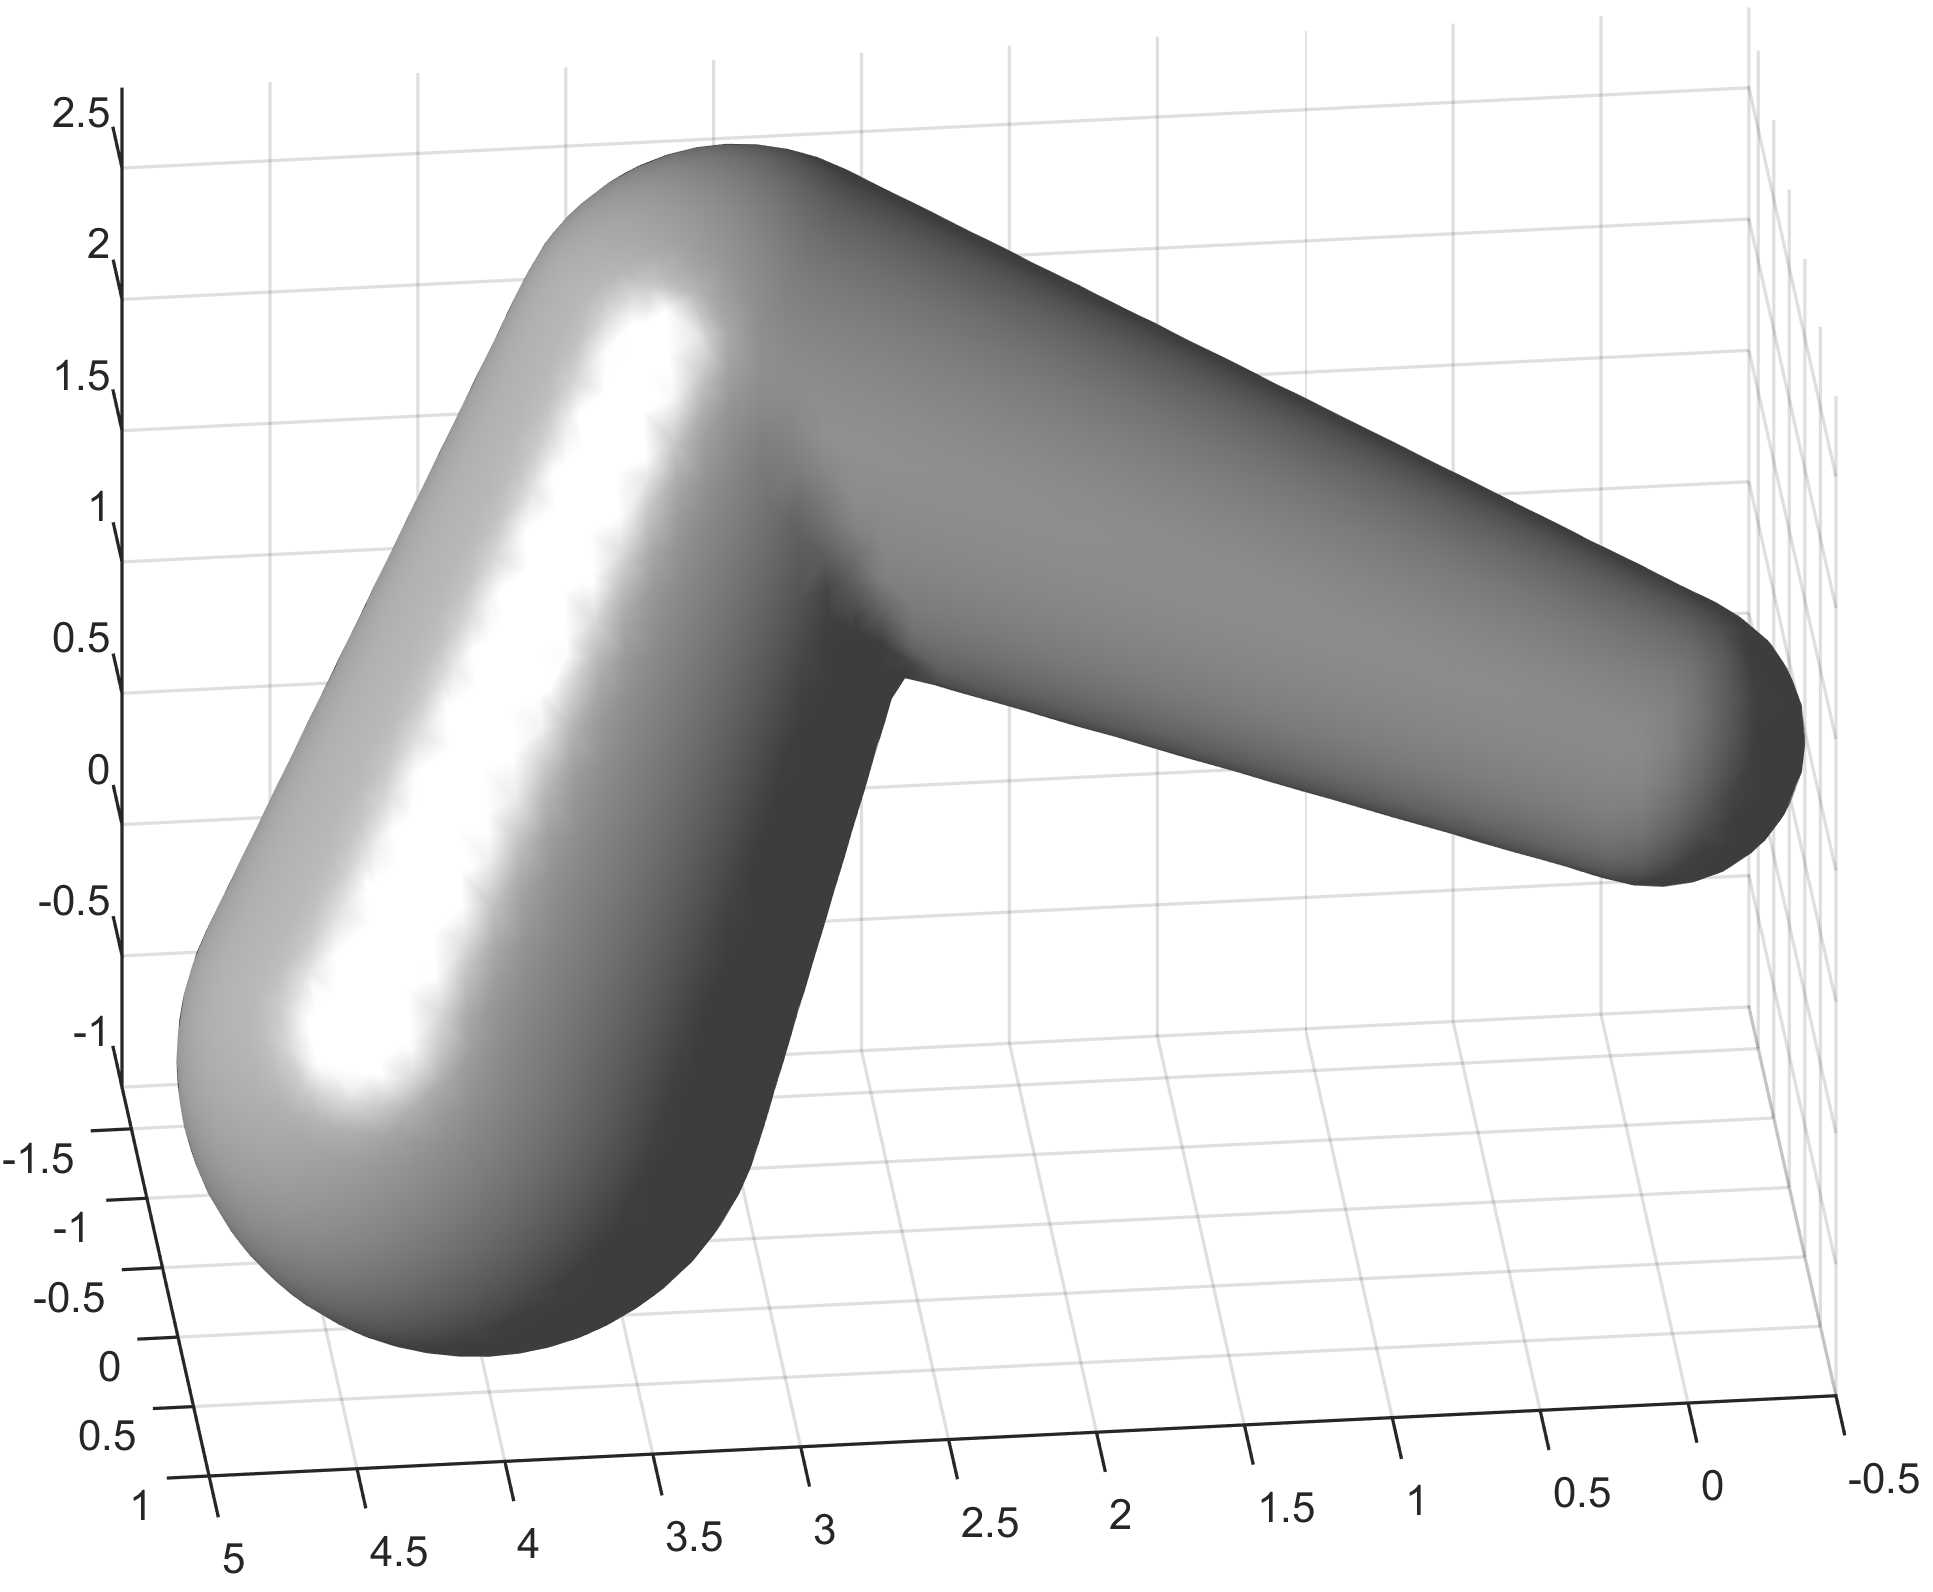
\includegraphics[width=0.4\textwidth]{figs/demo_union}
\end{center}

Similarly, \lstinline!sdf_blend! computes the blend operators, with the additional parameter $\theta$.
The function \lstinline!std_blend_theta_curve! can be used to get $\theta$ from $\alpha$, as suggested in section \ref{section:blendoperator}.

\begin{lstlisting}
alpha = pi / 2;
theta = sdf_blend_theta_curve( ...
  alpha, ...
  pi / 8, pi / 2, pi / 2, ...
  pi / 4, pi / 10, pi / 10, ...
  1 / 2, 1 / 2);
D = sdf_blend(D1, D2, theta);
D = reshape(D, size(X));
\end{lstlisting}

\begin{center}
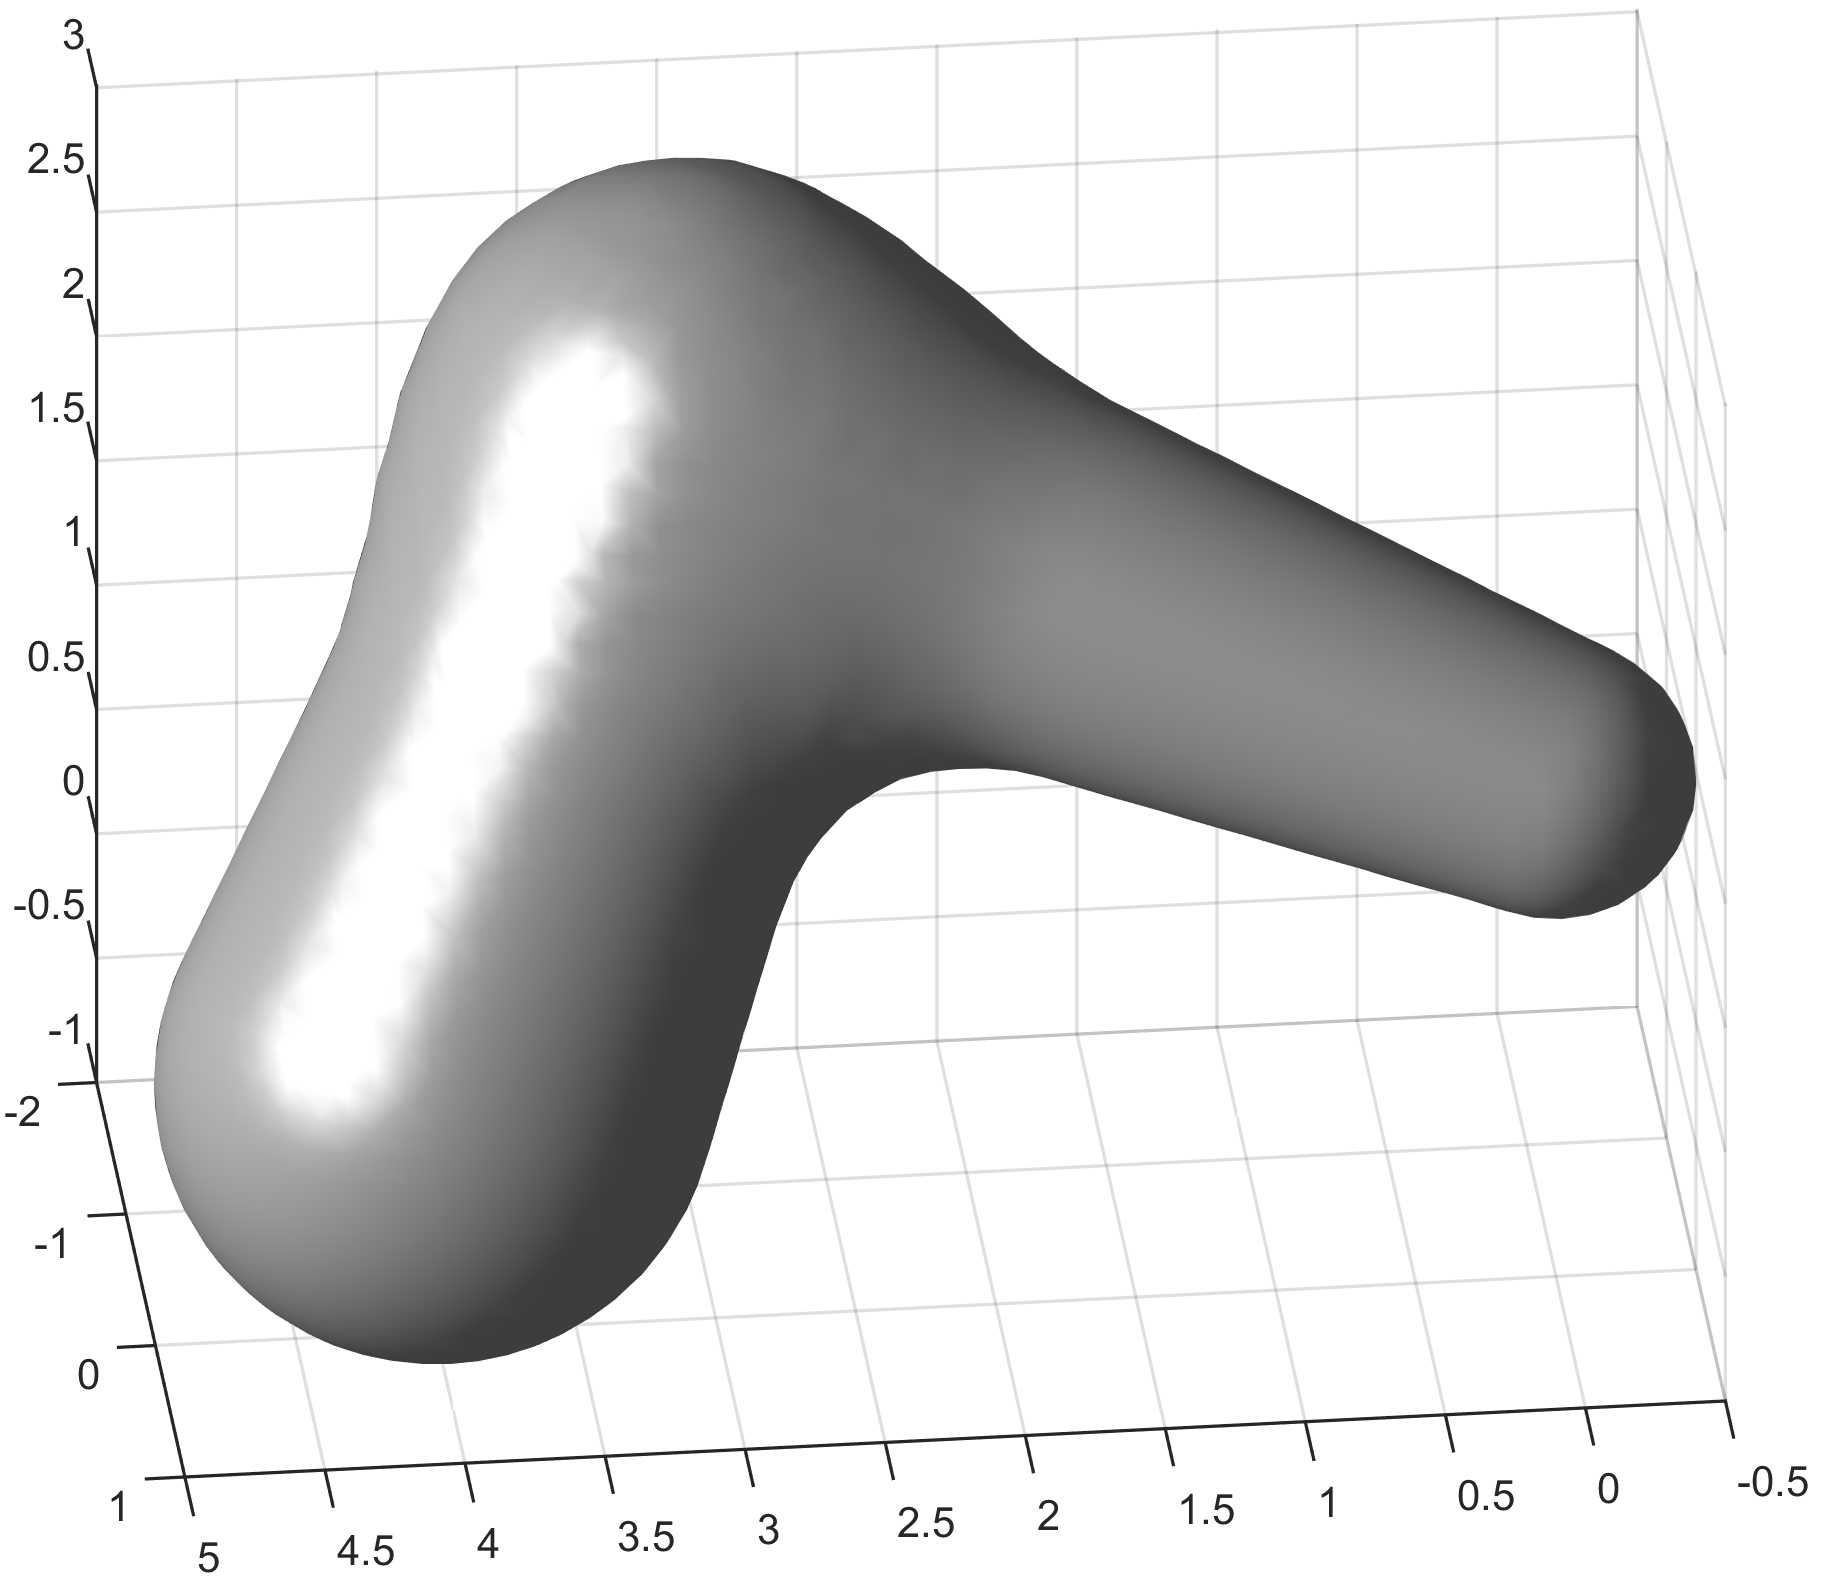
\includegraphics[width=0.4\textwidth]{figs/demo_blend}
\end{center}

As explained in section \ref{section:blendoperator}, our blend strategy is to set $\alpha$ as the angle between the two bones and interpolate between the union and the blend operators.


\subsection{Bones and traditional skinning}

Since a lot of various data is required to represent a mesh, we packed everything in a structure.
Vertices, faces, normals, skinning weights, HRBFs, spheres and some precomputations are stored in \lstinline!neutral.mat!.

As input, our algorithm gets the spheres used in hand tracking.
The method \lstinline!bone_axes! computes expected bone transformations.
Since the locations may not necessarily be consistent with our bone structure, the function \lstinline!bone_transforms! provides rigid transforms by constraining bone lengths.

\begin{lstlisting}
load('neutral.mat');
C = get_centers_somehow();
T = bone_transforms(mesh, C);
\end{lstlisting}

Once transforms are defined, \lstinline!skin_linear! and \lstinline!skin_dualquat! can be used to perform traditional skinning, as described in section \ref{section:traditional}.

\begin{lstlisting}
lbs = skin_linear(mesh, T);
\end{lstlisting}

\begin{center}
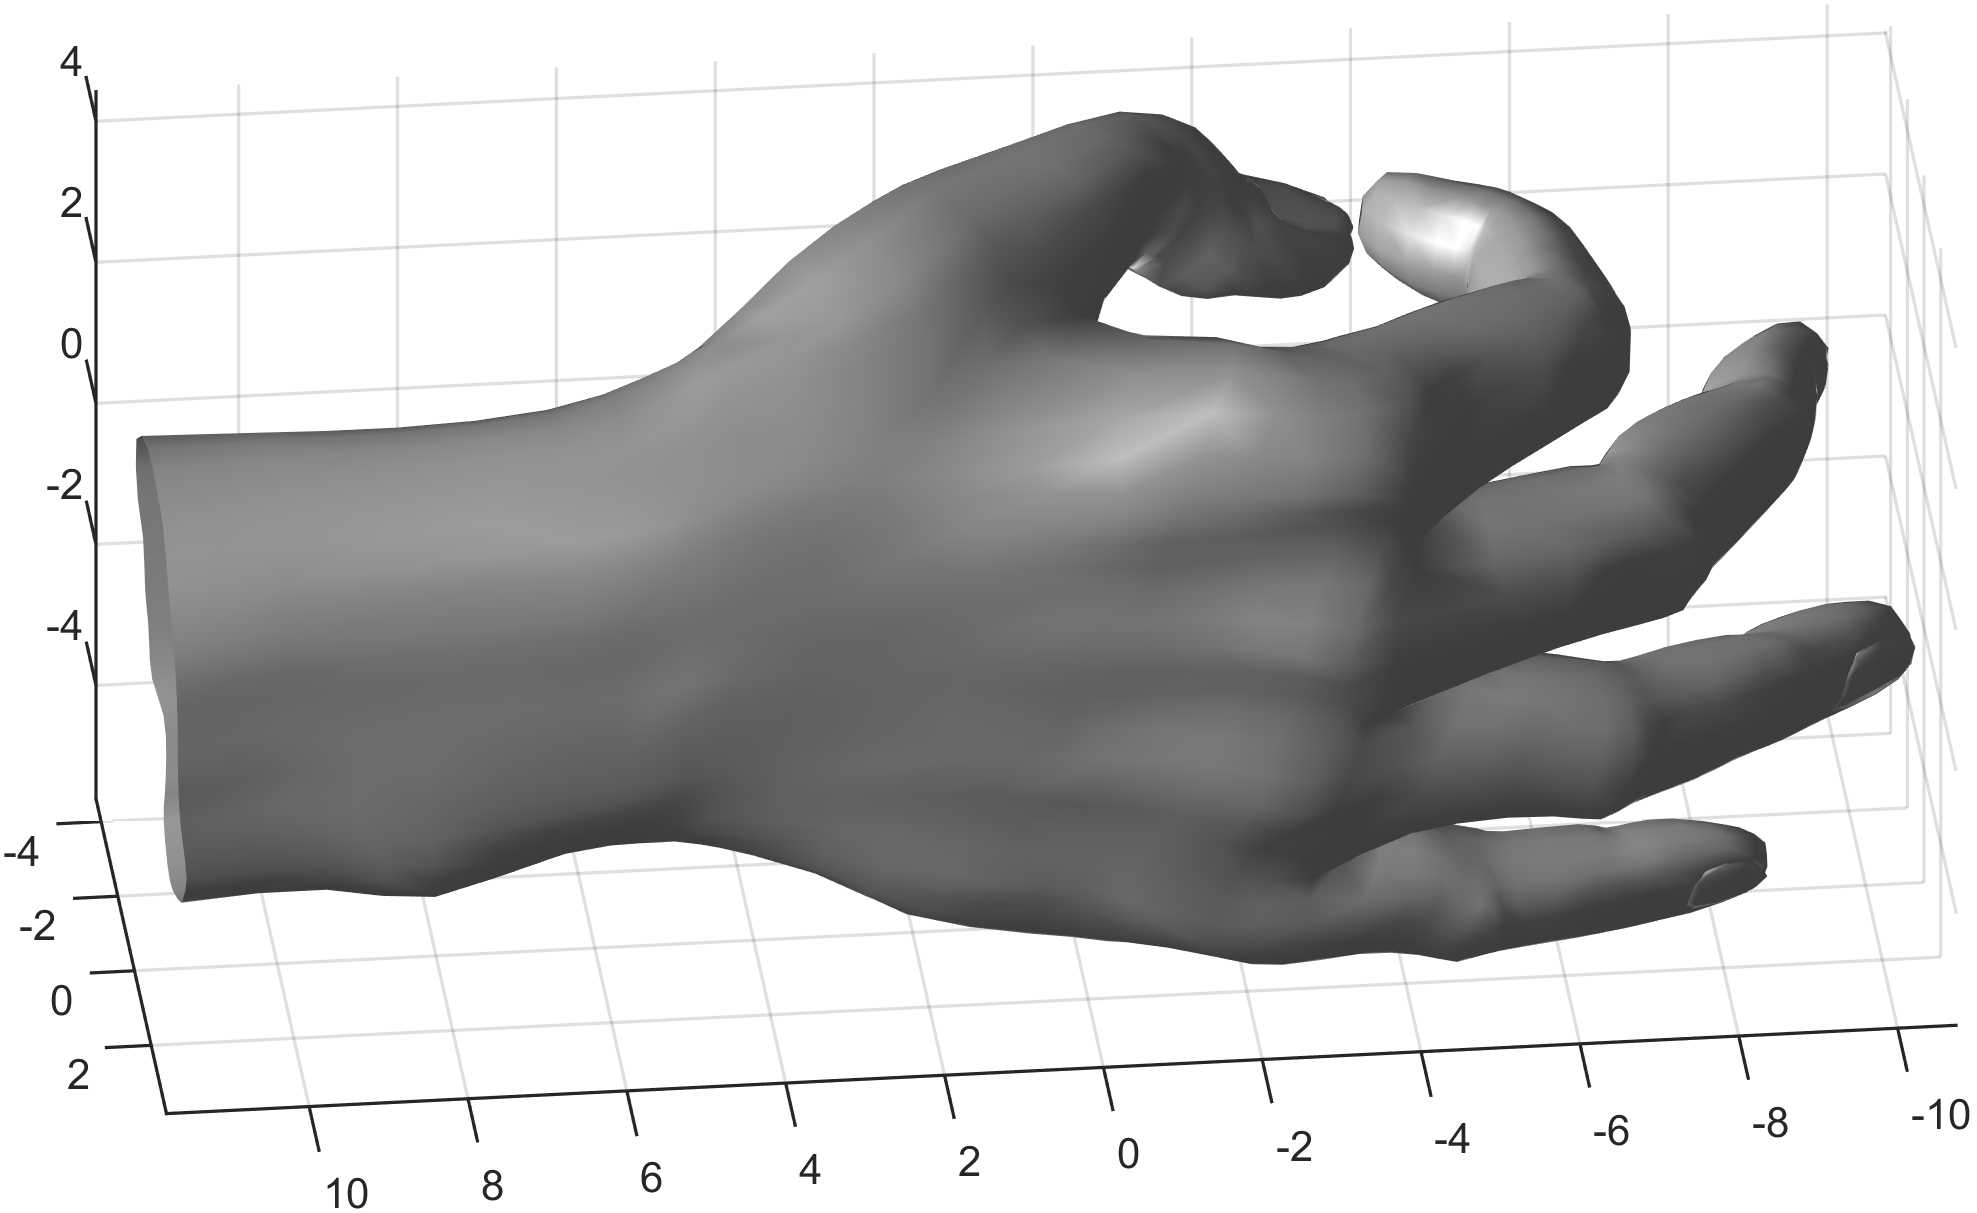
\includegraphics[width=0.4\textwidth]{figs/demo_linear}
\end{center}

\begin{lstlisting}
dqs = skin_dualquat(mesh, T);
\end{lstlisting}

\begin{center}
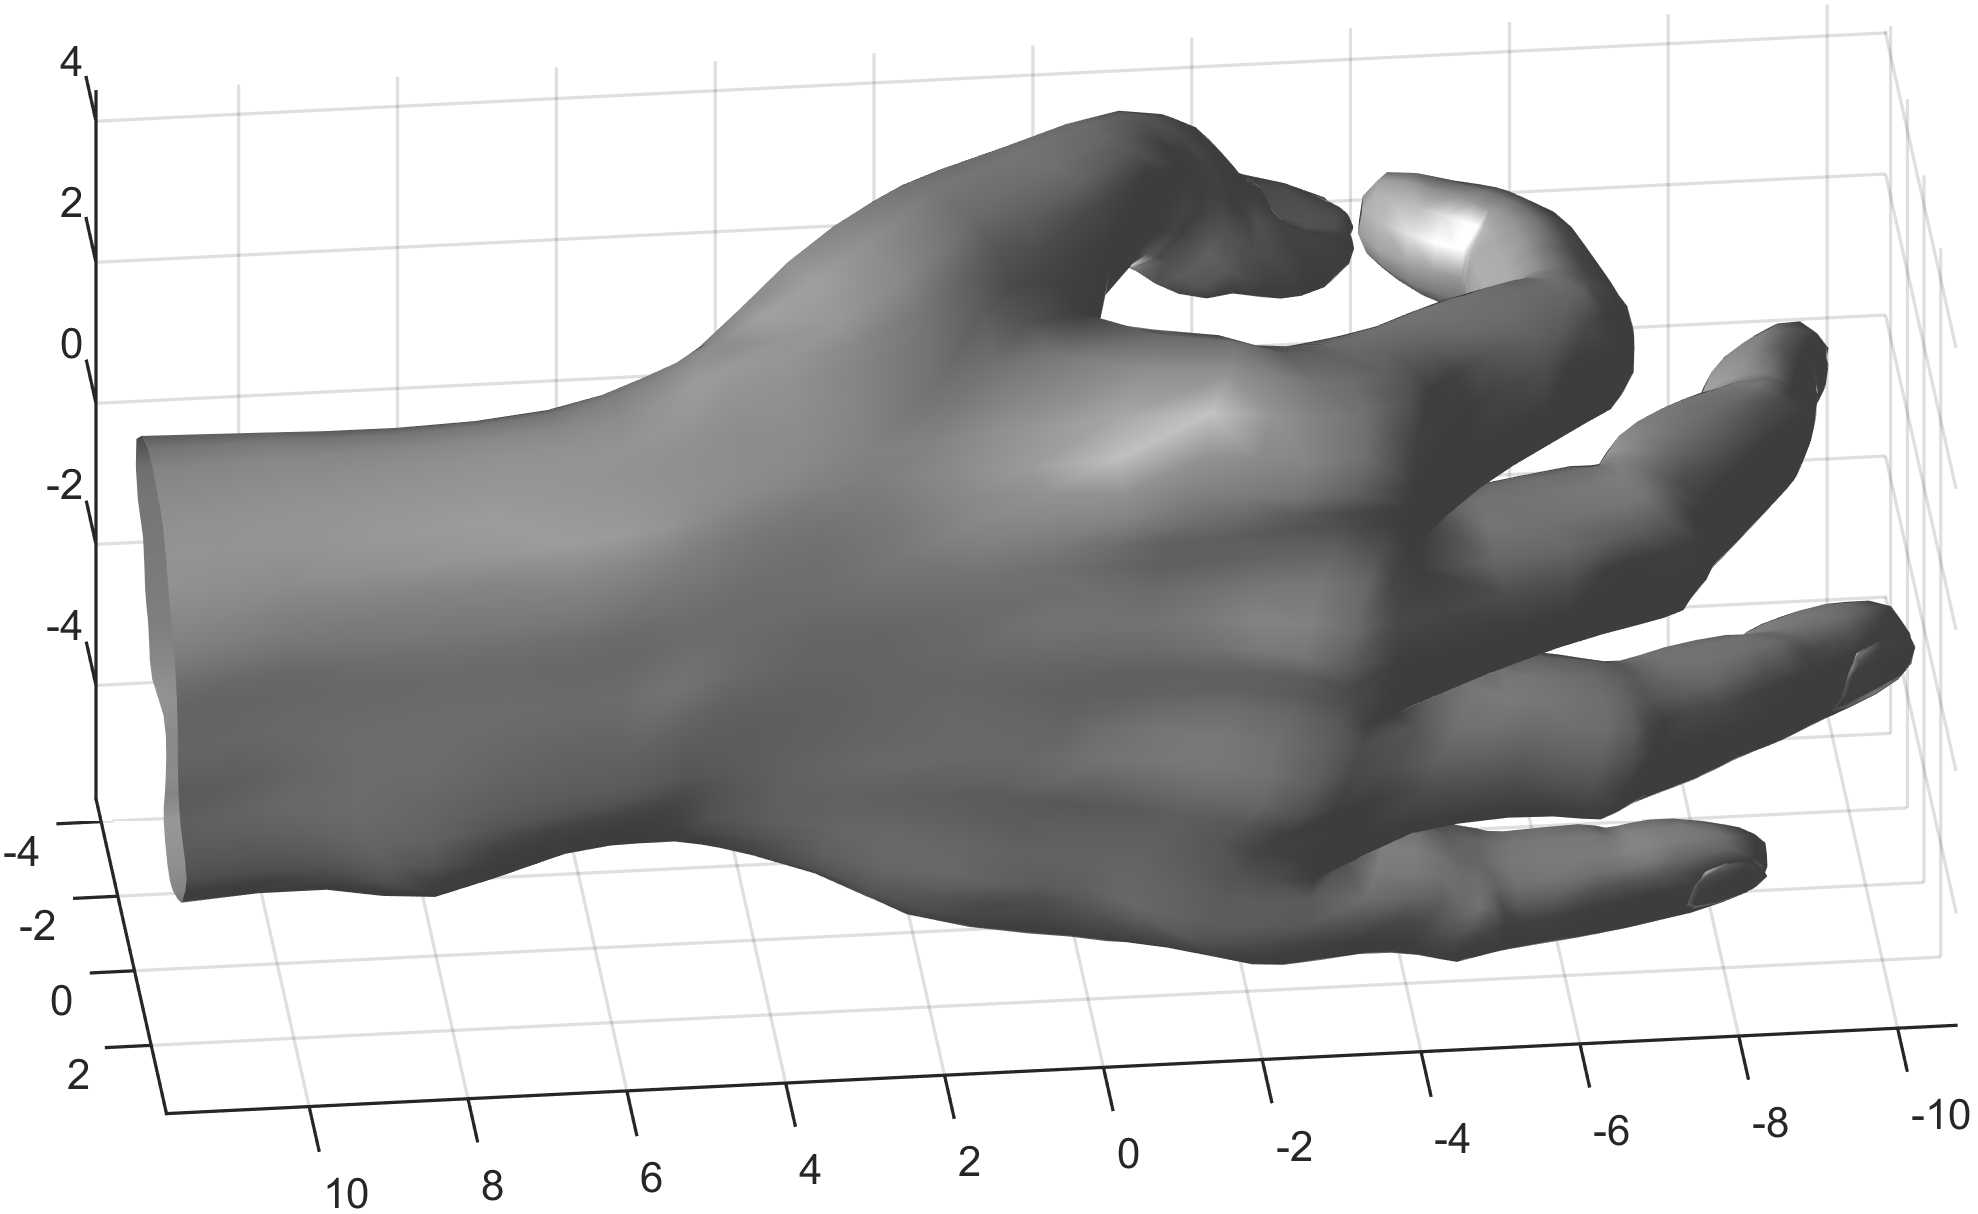
\includegraphics[width=0.4\textwidth]{figs/demo_dualquat}
\end{center}

Using a similar interface, implicit skinning can be also applied to a mesh.
The method \lstinline!skin_implicit! heavily relies on \lstinline!sdf_field!, which computes distances and gradients for every vertex.
As these two functions follows the algorithms described in this report in a straightforward manner, the code is self-explanatory.

\begin{lstlisting}
is = skin_implicit(mesh, T, 2);
\end{lstlisting}

\begin{center}
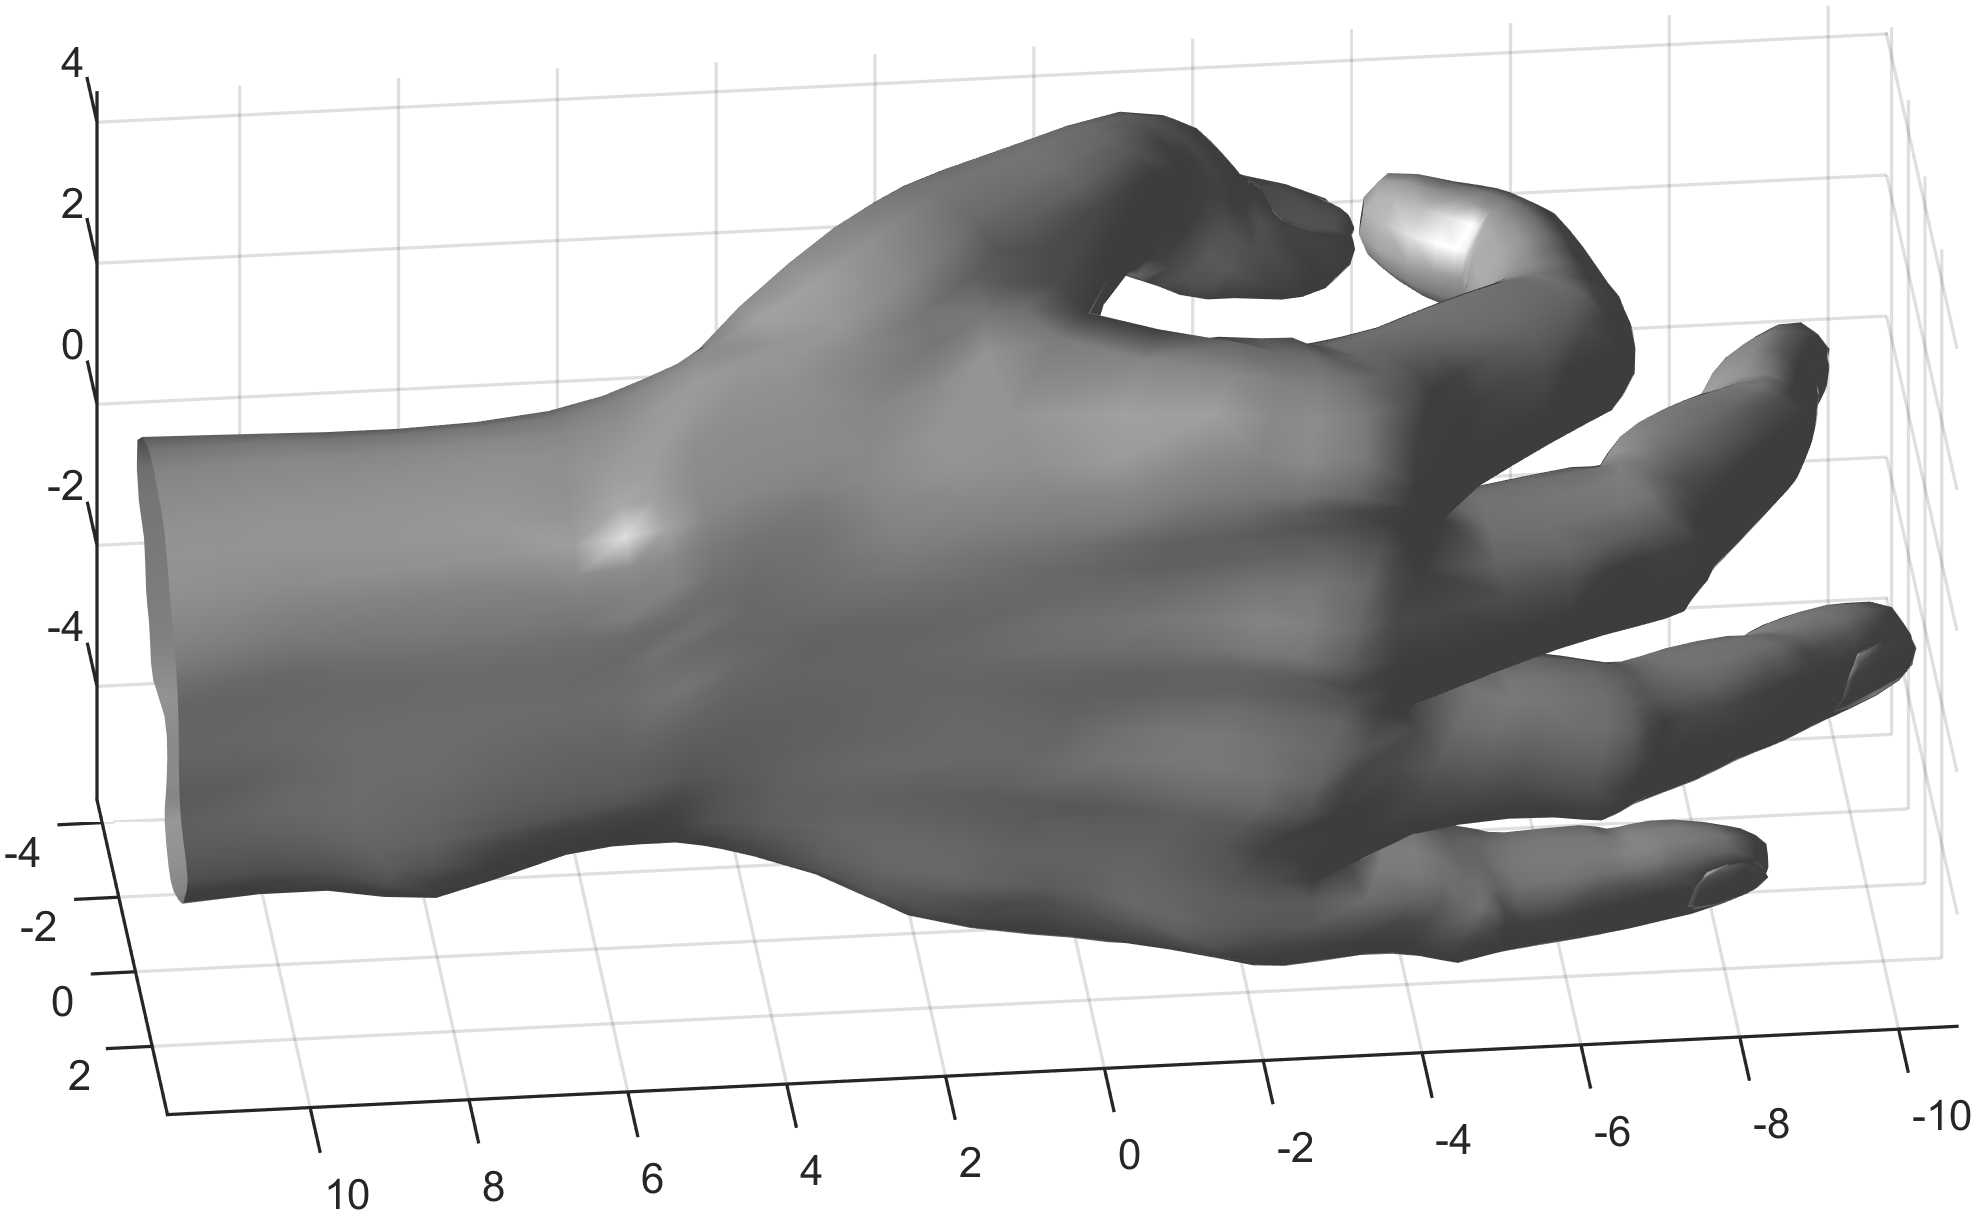
\includegraphics[width=0.4\textwidth]{figs/demo_implicit}
\end{center}


\subsection{Tests}

Finally, several scripts are provided, which are either demonstration code or preprocessing tools.
We encourage the reader to go through some of them to understand how the functions can be used.
Most of them were used to generate images of this report.

\begin{itemize}
\item
\lstinline!test_hrbf!, \lstinline!test_sphere!, \lstinline!test_operators! and \lstinline!test_bulge! provide complete example of local and global supported functions.
\item
\lstinline!test_2d_skinning!, \lstinline!test_compare_params! and \lstinline!test_compare_skinning! show differences between techniques and the impact of some parameters.
\item
\lstinline!test_generate_neutral! was used to compute and group all data related to skinning into \lstinline!neutral.mat!.
\lstinline!test_generate_hrbf! provides a better interface to tweak HRBF coefficients.
\item
\lstinline!test_export! generates \lstinline!neutral.obj! and \lstinline!neutral.skl!, which are used in the C++ implementation.
\end{itemize}


\section{C++ code}

\lstset{language=C++}

In order to test actual real-time performances of implicit skinning, a C++ implementation was developed.
Design goals are quite different from the MatLab version.
Most of the preprocessing code has not been ported to C++, since actual data can be exported from MatLab directly.
Moreover, some parts of the algorithm were modified to produce a simple yet functional code.

Since the goal is to provide real-time animation, some parts of the pipeline were simplified.
The major simplification is that the blend is not supported.
Only the union operator is implemented, mainly for time consideration, as the C++ implementation was achieved close to the deadline.
Hence, no bulging effect is available.

Another simplification is the absence of explicit optimization.
In order to have a clean and understandable code, only pure and straightforward C++ is used.
Vaillant's implementation, available on \href{http://rodolphe-vaillant.fr/?e=31}{his website}, precomputes most of the distance functions and use \emph{CUDA} to parallelize computations on GPU.
Hence, even with a simpler algorithm, we do not expect to reach similar performances.


\subsection{Skinning}

For simplicity's sake, the skinning library is contained in a single header \lstinline!skinning.h!.

Vector, matrices and dual quaternions are provided by \emph{OpenGL Mathematics}\cite{glm}, also known as \emph{GLM}.
This lightweight header-only library is designed to mimics \emph{OpenGL Shading Language} data structures.
Several extensions were added, which simplifies our code for dual quaternion skinning.

The other dependency is \emph{OpenMesh 5.1}\cite{openmesh} to read and manipulate meshes.
Its halfedge data structure provides efficient and intuitive access to vertices neighbors.

The \lstinline!HRBF! structure provides signed distance function for Hermite RBF.
While this is the only one implemented, any structure with a similar interface would work seamlessly with our library.
More precisely, any object with the following method is compatible:

\begin{lstlisting}
float apply(glm::vec3 const & point,
  glm::vec3 & gradient) const;
\end{lstlisting}

As explained above, the C++ code does not provide any precomputation.
As such, coefficients and centers must be provided, for instance using our MatLab implementation.

We also define the type \lstinline!Mesh!, which is an OpenMesh triangular mesh.
As long as normals are available, any mesh should work with our library.
The only requirement is the single precision for floating point numbers.
Our code assumes that \lstinline!glm::vec3! and \lstinline!Mesh::Point! are binary equivalents.

The main structure is \lstinline!Implicit!, which defines linear blend, dual quaternion and implicit skinning.
Given a mesh with skinning weights and desired bone transforms, geometry can be deformed with one of those algorithms:

\begin{lstlisting}
// Import HRBF somehow
Implicit<HRBF> implicit;
implicit.sdfs = /* ... */;

// Load mesh using OpenMesh
implicit.mesh = /* ... */;

// Import weights somehow
implicit.weights = /* ... */;
implicit.weights_bone = /* ... */;

// Initialize internal data
implicit.initialize();

// Ready to skin
implicit.transforms = /* ... */;
implicit.skin_linear();
implicit.skin_dualquat();
implicit.skin_implicit();
\end{lstlisting}


\subsection{Demo}

A minimal application is available in \lstinline!demo.cpp!, using \emph{OpenGL} to render the mesh.
\emph{OpenGL Extension Wrangler}\cite{glew}, also known as \emph{GLEW}, is used to load \emph{OpenGL functions}.
The context is created in a portable way with \emph{GLFW 3}\cite{glfw}.

Most of the code is used to set up the OpenGL context and render the scene.
As this is not the subject of this document, we will not discuss low-level rendering.
Anyway, the code was designed to have minimal performance penalty.

The mesh is loaded from \lstinline!neutral.obj!, which is a regular \emph{Wavefront OBJ file}.
Weights and HRBF coefficients are read from \lstinline!neutral.skl!, which is a custom file using an OBJ-like text-based encoding.
The \lstinline!test_export! script in MatLab generate these files from \lstinline!neutral.mat!.

\begin{center}
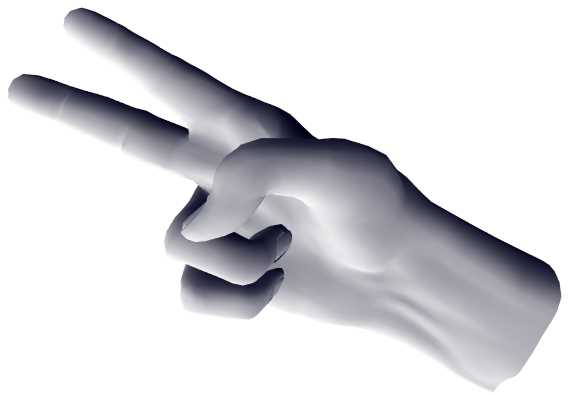
\includegraphics[width=0.45\textwidth]{figs/demo_cpp}
\end{center}

While the actual performances depends on hardware configuration, linear blend and dual quaternion skinning have similar efficiencies.
Implicit skinning is about 5 times slower, with approximately $100$ frames per seconds on our configuration.
Our computer has an \emph{Intel Core i7-4700HQ} which runs at $2.40$GHz.
However, as we explained before, the code is not optimized and could benefits from hardware parallelization.
On the other hand, the bulging effect is not implemented, which makes the code lighter.


\printbibliography


\end{multicols}

\end{document}
